% CS224 course-project presentation (Beamer, metropolis, 16:9). Build: `make` (figures + latexmk -xelatex).
\documentclass[aspectratio=169,11pt]{beamer}
\usetheme[progressbar=frametitle, numbering=fraction, sectionpage=progressbar, block=fill]{metropolis}
% Fira Sans is found by name through fontconfig/fonts.conf (exported by the Makefile);
% Fira Mono is set by file name so the upright face is used.
\setmonofont{FiraMono-Regular.otf}[BoldFont=FiraMono-Medium.otf, Scale=0.95]
% metropolis' title page is a \paperheight-tall minipage, 15.6pt taller than the frame (Overfull \vbox);
% same template, minus that overshoot.
\makeatletter
\setbeamertemplate{title page}{
  \begin{minipage}[b][\dimexpr\paperheight-16pt\relax]{\textwidth}
    \ifx\inserttitlegraphic\@empty\else\usebeamertemplate*{title graphic}\fi
    \vfill%
    \ifx\inserttitle\@empty\else\usebeamertemplate*{title}\fi
    \ifx\insertsubtitle\@empty\else\usebeamertemplate*{subtitle}\fi
    \usebeamertemplate*{title separator}
    \ifx\beamer@shortauthor\@empty\else\usebeamertemplate*{author}\fi
    \ifx\insertdate\@empty\else\usebeamertemplate*{date}\fi
    \ifx\insertinstitute\@empty\else\usebeamertemplate*{institute}\fi
    \vfill
    \vspace*{1mm}
  \end{minipage}
}
\makeatother

\usepackage{booktabs}
\usepackage{listings}
\usepackage{tikz}
\usetikzlibrary{positioning, arrows.meta, fit, calc, backgrounds, shapes.misc, decorations.pathreplacing}
\usepackage{appendixnumberbeamer}
\usepackage{pifont}

% ---- palette (Okabe-Ito accents + muted box palette) ----------------------------
\definecolor{Ink}{HTML}{26303A}
\definecolor{OIblue}{HTML}{0072B2}
\definecolor{OIsky}{HTML}{56B4E9}
\definecolor{OIorange}{HTML}{E69F00}
\definecolor{OIgreen}{HTML}{009E73}
\definecolor{OIvermil}{HTML}{D55E00}
\definecolor{OIpurple}{HTML}{CC79A7}
\definecolor{HeroFill}{HTML}{E9F1FB}\definecolor{HeroDraw}{HTML}{2F6FB0}
\definecolor{DataFill}{HTML}{E6F3EE}\definecolor{DataDraw}{HTML}{2E8B7A}
\definecolor{WarnFill}{HTML}{FBF1E3}\definecolor{WarnDraw}{HTML}{BE8A2E}
\definecolor{NeutFill}{HTML}{F2F4F8}\definecolor{NeutDraw}{HTML}{5A6472}
\setbeamercolor{alerted text}{fg=OIvermil}

% ---- small helpers --------------------------------------------------------------
\newcommand{\cmark}{\textcolor{OIgreen}{\ding{51}}}
\newcommand{\xmark}{\textcolor{OIvermil}{\ding{55}}}
\newcommand{\code}[1]{\texttt{\small #1}}
% Numbered per-frame citations (user 2026-11-24 19:05 / 19:45). \sref{key} or \sref{key1,key2} prints a superscript
% number at the mention and registers the key for this frame; the frame footer lists "n short-form" (short forms:
% sources.tex, keys = report/final_en/references.bib keys or url-/cs224- entries). Numbering restarts on every
% frame, in order of first mention. An unknown key is a LaTeX error. Every printed superscript and every footer
% entry writes "B|F <page> <n> <key>" to build/main.sref (non-immediate \write, so only material that is really
% shipped counts); tools/check_citations.py (make check) fails when the two sets differ on any page.
\makeatletter
\newwrite\sref@out
\AtBeginDocument{\immediate\openout\sref@out=\jobname.sref}
\newcount\sref@gen
\newcount\sref@n
\newcommand{\sref@foot}{}
\newcommand{\sref@reset}{\global\advance\sref@gen\@ne\global\sref@n\z@\gdef\sref@foot{}}
\newcommand{\sref@one}[1]{%
  \edef\sref@key{#1}%
  \ifcsname bib-\sref@key\endcsname\else\errmessage{sref: unknown source key '\sref@key' (add it to sources.tex)}\fi
  \ifcsname sref@\the\sref@gen @\sref@key\endcsname\else
    \global\advance\sref@n\@ne
    \expandafter\xdef\csname sref@\the\sref@gen @\sref@key\endcsname{\the\sref@n}%
    \xdef\sref@foot{\unexpanded\expandafter{\sref@foot}\noexpand\sref@entry{\the\sref@n}{\sref@key}}%
  \fi
  \edef\sref@num{\csname sref@\the\sref@gen @\sref@key\endcsname}%
  \sref@num
  \edef\sref@do{\write\sref@out{B \noexpand\thepage\space\sref@num\space\sref@key}}\sref@do}
\newcommand{\sref}[1]{\textsuperscript{\def\sref@sep{}\@for\sref@k:=#1\do{\sref@sep\sref@one{\sref@k}\def\sref@sep{,}}}}
\newcommand{\sref@entry}[2]{\mbox{\textsuperscript{#1}\,\bib{#2}}\hspace{0.9em plus 0.3em}%
  \write\sref@out{F \thepage\space#1\space#2}}
\BeforeBeginEnvironment{frame}{\sref@reset}
% footer: grey 6.5 pt, up to two lines below the body, left of the page number; reset after printing
% (the box height goes to main.sref as "H <page> <pt>"; check_citations.py fails above two lines)
\newsavebox{\sref@box}
\setbeamertemplate{frame footer}{%
  \ifx\sref@foot\@empty\else
    \sbox{\sref@box}{\parbox[t]{0.88\textwidth}{\raggedright\fontsize{6.5}{7.4}\selectfont\color{NeutDraw}\sref@foot}}%
    \edef\sref@do{\write\sref@out{H \noexpand\thepage\space\strip@pt\dimexpr\ht\sref@box+\dp\sref@box\relax}}\sref@do
    \smash{\usebox{\sref@box}}%
  \fi
  \sref@reset}
\makeatother
% generated by figures/make_figures.py -- do not edit
% \res{<method key>-<layer>}{<metric>}: p r f1 macro spec ci n tp fp tn fn; paired vs layer1: base d
% lost gained flips; unknown or pending -> \textit{pending}
\providecommand{\res}[2]{\ifcsname res-#1-#2\endcsname\csname res-#1-#2\endcsname\else\textit{pending}\fi}
\expandafter\def\csname res-grep-layer1-p\endcsname{0.658}
\expandafter\def\csname res-grep-layer1-r\endcsname{0.870}
\expandafter\def\csname res-grep-layer1-f1\endcsname{0.749}
\expandafter\def\csname res-grep-layer1-macro\endcsname{0.701}
\expandafter\def\csname res-grep-layer1-spec\endcsname{0.548}
\expandafter\def\csname res-grep-layer1-n\endcsname{2,656}
\expandafter\def\csname res-grep-layer1-tp\endcsname{1,155}
\expandafter\def\csname res-grep-layer1-fp\endcsname{600}
\expandafter\def\csname res-grep-layer1-tn\endcsname{728}
\expandafter\def\csname res-grep-layer1-fn\endcsname{173}
\expandafter\def\csname res-grep-layer1-ci\endcsname{[0.685, 0.717]}
\expandafter\def\csname res-grep-layer1-r_c_alloc\endcsname{0.923}
\expandafter\def\csname res-grep-layer1-r_cpp_new\endcsname{0.939}
\expandafter\def\csname res-grep-layer1-r_destructor\endcsname{0.500}
\expandafter\def\csname res-grep-layer1-r_realloc_fail\endcsname{0.000}
\expandafter\def\csname res-grep-layer3-p\endcsname{--}
\expandafter\def\csname res-grep-layer3-r\endcsname{0.000}
\expandafter\def\csname res-grep-layer3-f1\endcsname{0.000}
\expandafter\def\csname res-grep-layer3-macro\endcsname{0.333}
\expandafter\def\csname res-grep-layer3-spec\endcsname{1.000}
\expandafter\def\csname res-grep-layer3-base\endcsname{0.701}
\expandafter\def\csname res-grep-layer3-n\endcsname{2,656}
\expandafter\def\csname res-grep-layer3-tp\endcsname{0}
\expandafter\def\csname res-grep-layer3-fp\endcsname{0}
\expandafter\def\csname res-grep-layer3-tn\endcsname{1,328}
\expandafter\def\csname res-grep-layer3-fn\endcsname{1,328}
\expandafter\def\csname res-grep-layer3-lost\endcsname{1,155}
\expandafter\def\csname res-grep-layer3-gained\endcsname{0}
\expandafter\def\csname res-grep-layer3-flips\endcsname{1,755}
\expandafter\def\csname res-grep-layer3-d\endcsname{$-$0.368}
\expandafter\def\csname res-grep-layer3-ci\endcsname{[0.333, 0.333]}
\expandafter\def\csname res-grep-layer3-r_c_alloc\endcsname{0.000}
\expandafter\def\csname res-grep-layer3-r_cpp_new\endcsname{0.000}
\expandafter\def\csname res-grep-layer3-r_destructor\endcsname{0.000}
\expandafter\def\csname res-grep-layer3-r_realloc_fail\endcsname{0.000}
\expandafter\def\csname res-grep-placebo-p\endcsname{0.658}
\expandafter\def\csname res-grep-placebo-r\endcsname{0.870}
\expandafter\def\csname res-grep-placebo-f1\endcsname{0.749}
\expandafter\def\csname res-grep-placebo-macro\endcsname{0.701}
\expandafter\def\csname res-grep-placebo-spec\endcsname{0.548}
\expandafter\def\csname res-grep-placebo-base\endcsname{0.701}
\expandafter\def\csname res-grep-placebo-n\endcsname{2,656}
\expandafter\def\csname res-grep-placebo-tp\endcsname{1,155}
\expandafter\def\csname res-grep-placebo-fp\endcsname{600}
\expandafter\def\csname res-grep-placebo-tn\endcsname{728}
\expandafter\def\csname res-grep-placebo-fn\endcsname{173}
\expandafter\def\csname res-grep-placebo-lost\endcsname{0}
\expandafter\def\csname res-grep-placebo-gained\endcsname{0}
\expandafter\def\csname res-grep-placebo-flips\endcsname{0}
\expandafter\def\csname res-grep-placebo-d\endcsname{$\pm$0.000}
\expandafter\def\csname res-grep-placebo-ci\endcsname{[0.685, 0.717]}
\expandafter\def\csname res-grep-placebo-r_c_alloc\endcsname{0.923}
\expandafter\def\csname res-grep-placebo-r_cpp_new\endcsname{0.939}
\expandafter\def\csname res-grep-placebo-r_destructor\endcsname{0.500}
\expandafter\def\csname res-grep-placebo-r_realloc_fail\endcsname{0.000}
\expandafter\def\csname res-grep-original-p\endcsname{1.000}
\expandafter\def\csname res-grep-original-r\endcsname{0.870}
\expandafter\def\csname res-grep-original-f1\endcsname{0.930}
\expandafter\def\csname res-grep-original-macro\endcsname{0.935}
\expandafter\def\csname res-grep-original-spec\endcsname{1.000}
\expandafter\def\csname res-grep-original-base\endcsname{0.701}
\expandafter\def\csname res-grep-original-n\endcsname{2,656}
\expandafter\def\csname res-grep-original-tp\endcsname{1,155}
\expandafter\def\csname res-grep-original-fp\endcsname{0}
\expandafter\def\csname res-grep-original-tn\endcsname{1,328}
\expandafter\def\csname res-grep-original-fn\endcsname{173}
\expandafter\def\csname res-grep-original-lost\endcsname{0}
\expandafter\def\csname res-grep-original-gained\endcsname{0}
\expandafter\def\csname res-grep-original-flips\endcsname{600}
\expandafter\def\csname res-grep-original-d\endcsname{+0.233}
\expandafter\def\csname res-grep-original-ci\endcsname{[0.906, 0.955]}
\expandafter\def\csname res-grep-original-r_c_alloc\endcsname{0.923}
\expandafter\def\csname res-grep-original-r_cpp_new\endcsname{0.939}
\expandafter\def\csname res-grep-original-r_destructor\endcsname{0.500}
\expandafter\def\csname res-grep-original-r_realloc_fail\endcsname{0.000}
\expandafter\def\csname res-cppcheck-layer1-p\endcsname{0.897}
\expandafter\def\csname res-cppcheck-layer1-r\endcsname{0.171}
\expandafter\def\csname res-cppcheck-layer1-f1\endcsname{0.287}
\expandafter\def\csname res-cppcheck-layer1-macro\endcsname{0.493}
\expandafter\def\csname res-cppcheck-layer1-spec\endcsname{0.980}
\expandafter\def\csname res-cppcheck-layer1-n\endcsname{2,656}
\expandafter\def\csname res-cppcheck-layer1-tp\endcsname{227}
\expandafter\def\csname res-cppcheck-layer1-fp\endcsname{26}
\expandafter\def\csname res-cppcheck-layer1-tn\endcsname{1,302}
\expandafter\def\csname res-cppcheck-layer1-fn\endcsname{1,101}
\expandafter\def\csname res-cppcheck-layer1-ci\endcsname{[0.436, 0.553]}
\expandafter\def\csname res-cppcheck-layer1-r_c_alloc\endcsname{0.067}
\expandafter\def\csname res-cppcheck-layer1-r_cpp_new\endcsname{0.197}
\expandafter\def\csname res-cppcheck-layer1-r_destructor\endcsname{0.000}
\expandafter\def\csname res-cppcheck-layer1-r_realloc_fail\endcsname{1.000}
\expandafter\def\csname res-cppcheck-layer3-p\endcsname{0.897}
\expandafter\def\csname res-cppcheck-layer3-r\endcsname{0.171}
\expandafter\def\csname res-cppcheck-layer3-f1\endcsname{0.287}
\expandafter\def\csname res-cppcheck-layer3-macro\endcsname{0.493}
\expandafter\def\csname res-cppcheck-layer3-spec\endcsname{0.980}
\expandafter\def\csname res-cppcheck-layer3-base\endcsname{0.493}
\expandafter\def\csname res-cppcheck-layer3-n\endcsname{2,656}
\expandafter\def\csname res-cppcheck-layer3-tp\endcsname{227}
\expandafter\def\csname res-cppcheck-layer3-fp\endcsname{26}
\expandafter\def\csname res-cppcheck-layer3-tn\endcsname{1,302}
\expandafter\def\csname res-cppcheck-layer3-fn\endcsname{1,101}
\expandafter\def\csname res-cppcheck-layer3-lost\endcsname{0}
\expandafter\def\csname res-cppcheck-layer3-gained\endcsname{0}
\expandafter\def\csname res-cppcheck-layer3-flips\endcsname{0}
\expandafter\def\csname res-cppcheck-layer3-d\endcsname{$\pm$0.000}
\expandafter\def\csname res-cppcheck-layer3-ci\endcsname{[0.436, 0.553]}
\expandafter\def\csname res-cppcheck-layer3-r_c_alloc\endcsname{0.067}
\expandafter\def\csname res-cppcheck-layer3-r_cpp_new\endcsname{0.197}
\expandafter\def\csname res-cppcheck-layer3-r_destructor\endcsname{0.000}
\expandafter\def\csname res-cppcheck-layer3-r_realloc_fail\endcsname{1.000}
\expandafter\def\csname res-cppcheck-placebo-p\endcsname{0.897}
\expandafter\def\csname res-cppcheck-placebo-r\endcsname{0.171}
\expandafter\def\csname res-cppcheck-placebo-f1\endcsname{0.287}
\expandafter\def\csname res-cppcheck-placebo-macro\endcsname{0.493}
\expandafter\def\csname res-cppcheck-placebo-spec\endcsname{0.980}
\expandafter\def\csname res-cppcheck-placebo-base\endcsname{0.493}
\expandafter\def\csname res-cppcheck-placebo-n\endcsname{2,656}
\expandafter\def\csname res-cppcheck-placebo-tp\endcsname{227}
\expandafter\def\csname res-cppcheck-placebo-fp\endcsname{26}
\expandafter\def\csname res-cppcheck-placebo-tn\endcsname{1,302}
\expandafter\def\csname res-cppcheck-placebo-fn\endcsname{1,101}
\expandafter\def\csname res-cppcheck-placebo-lost\endcsname{0}
\expandafter\def\csname res-cppcheck-placebo-gained\endcsname{0}
\expandafter\def\csname res-cppcheck-placebo-flips\endcsname{0}
\expandafter\def\csname res-cppcheck-placebo-d\endcsname{$\pm$0.000}
\expandafter\def\csname res-cppcheck-placebo-ci\endcsname{[0.436, 0.553]}
\expandafter\def\csname res-cppcheck-placebo-r_c_alloc\endcsname{0.067}
\expandafter\def\csname res-cppcheck-placebo-r_cpp_new\endcsname{0.197}
\expandafter\def\csname res-cppcheck-placebo-r_destructor\endcsname{0.000}
\expandafter\def\csname res-cppcheck-placebo-r_realloc_fail\endcsname{1.000}
\expandafter\def\csname res-cppcheck-original-p\endcsname{0.652}
\expandafter\def\csname res-cppcheck-original-r\endcsname{0.171}
\expandafter\def\csname res-cppcheck-original-f1\endcsname{0.271}
\expandafter\def\csname res-cppcheck-original-macro\endcsname{0.467}
\expandafter\def\csname res-cppcheck-original-spec\endcsname{0.909}
\expandafter\def\csname res-cppcheck-original-base\endcsname{0.493}
\expandafter\def\csname res-cppcheck-original-n\endcsname{2,656}
\expandafter\def\csname res-cppcheck-original-tp\endcsname{227}
\expandafter\def\csname res-cppcheck-original-fp\endcsname{121}
\expandafter\def\csname res-cppcheck-original-tn\endcsname{1,207}
\expandafter\def\csname res-cppcheck-original-fn\endcsname{1,101}
\expandafter\def\csname res-cppcheck-original-lost\endcsname{0}
\expandafter\def\csname res-cppcheck-original-gained\endcsname{95}
\expandafter\def\csname res-cppcheck-original-flips\endcsname{95}
\expandafter\def\csname res-cppcheck-original-d\endcsname{$-$0.025}
\expandafter\def\csname res-cppcheck-original-ci\endcsname{[0.421, 0.518]}
\expandafter\def\csname res-cppcheck-original-r_c_alloc\endcsname{0.067}
\expandafter\def\csname res-cppcheck-original-r_cpp_new\endcsname{0.197}
\expandafter\def\csname res-cppcheck-original-r_destructor\endcsname{0.000}
\expandafter\def\csname res-cppcheck-original-r_realloc_fail\endcsname{1.000}
\expandafter\def\csname res-clang_sa-layer1-p\endcsname{0.928}
\expandafter\def\csname res-clang_sa-layer1-r\endcsname{0.771}
\expandafter\def\csname res-clang_sa-layer1-f1\endcsname{0.842}
\expandafter\def\csname res-clang_sa-layer1-macro\endcsname{0.855}
\expandafter\def\csname res-clang_sa-layer1-spec\endcsname{0.941}
\expandafter\def\csname res-clang_sa-layer1-n\endcsname{2,656}
\expandafter\def\csname res-clang_sa-layer1-tp\endcsname{1,024}
\expandafter\def\csname res-clang_sa-layer1-fp\endcsname{79}
\expandafter\def\csname res-clang_sa-layer1-tn\endcsname{1,249}
\expandafter\def\csname res-clang_sa-layer1-fn\endcsname{304}
\expandafter\def\csname res-clang_sa-layer1-ci\endcsname{[0.806, 0.899]}
\expandafter\def\csname res-clang_sa-layer1-r_c_alloc\endcsname{0.897}
\expandafter\def\csname res-clang_sa-layer1-r_cpp_new\endcsname{0.519}
\expandafter\def\csname res-clang_sa-layer1-r_destructor\endcsname{0.000}
\expandafter\def\csname res-clang_sa-layer1-r_realloc_fail\endcsname{1.000}
\expandafter\def\csname res-clang_sa-layer3-p\endcsname{0.928}
\expandafter\def\csname res-clang_sa-layer3-r\endcsname{0.771}
\expandafter\def\csname res-clang_sa-layer3-f1\endcsname{0.842}
\expandafter\def\csname res-clang_sa-layer3-macro\endcsname{0.855}
\expandafter\def\csname res-clang_sa-layer3-spec\endcsname{0.941}
\expandafter\def\csname res-clang_sa-layer3-base\endcsname{0.855}
\expandafter\def\csname res-clang_sa-layer3-n\endcsname{2,656}
\expandafter\def\csname res-clang_sa-layer3-tp\endcsname{1,024}
\expandafter\def\csname res-clang_sa-layer3-fp\endcsname{79}
\expandafter\def\csname res-clang_sa-layer3-tn\endcsname{1,249}
\expandafter\def\csname res-clang_sa-layer3-fn\endcsname{304}
\expandafter\def\csname res-clang_sa-layer3-lost\endcsname{0}
\expandafter\def\csname res-clang_sa-layer3-gained\endcsname{0}
\expandafter\def\csname res-clang_sa-layer3-flips\endcsname{0}
\expandafter\def\csname res-clang_sa-layer3-d\endcsname{$\pm$0.000}
\expandafter\def\csname res-clang_sa-layer3-ci\endcsname{[0.806, 0.899]}
\expandafter\def\csname res-clang_sa-layer3-r_c_alloc\endcsname{0.897}
\expandafter\def\csname res-clang_sa-layer3-r_cpp_new\endcsname{0.519}
\expandafter\def\csname res-clang_sa-layer3-r_destructor\endcsname{0.000}
\expandafter\def\csname res-clang_sa-layer3-r_realloc_fail\endcsname{1.000}
\expandafter\def\csname res-clang_sa-placebo-p\endcsname{0.928}
\expandafter\def\csname res-clang_sa-placebo-r\endcsname{0.771}
\expandafter\def\csname res-clang_sa-placebo-f1\endcsname{0.842}
\expandafter\def\csname res-clang_sa-placebo-macro\endcsname{0.855}
\expandafter\def\csname res-clang_sa-placebo-spec\endcsname{0.941}
\expandafter\def\csname res-clang_sa-placebo-base\endcsname{0.855}
\expandafter\def\csname res-clang_sa-placebo-n\endcsname{2,656}
\expandafter\def\csname res-clang_sa-placebo-tp\endcsname{1,024}
\expandafter\def\csname res-clang_sa-placebo-fp\endcsname{79}
\expandafter\def\csname res-clang_sa-placebo-tn\endcsname{1,249}
\expandafter\def\csname res-clang_sa-placebo-fn\endcsname{304}
\expandafter\def\csname res-clang_sa-placebo-lost\endcsname{0}
\expandafter\def\csname res-clang_sa-placebo-gained\endcsname{0}
\expandafter\def\csname res-clang_sa-placebo-flips\endcsname{0}
\expandafter\def\csname res-clang_sa-placebo-d\endcsname{$\pm$0.000}
\expandafter\def\csname res-clang_sa-placebo-ci\endcsname{[0.806, 0.899]}
\expandafter\def\csname res-clang_sa-placebo-r_c_alloc\endcsname{0.897}
\expandafter\def\csname res-clang_sa-placebo-r_cpp_new\endcsname{0.519}
\expandafter\def\csname res-clang_sa-placebo-r_destructor\endcsname{0.000}
\expandafter\def\csname res-clang_sa-placebo-r_realloc_fail\endcsname{1.000}
\expandafter\def\csname res-clang_sa-original-p\endcsname{0.859}
\expandafter\def\csname res-clang_sa-original-r\endcsname{0.771}
\expandafter\def\csname res-clang_sa-original-f1\endcsname{0.813}
\expandafter\def\csname res-clang_sa-original-macro\endcsname{0.822}
\expandafter\def\csname res-clang_sa-original-spec\endcsname{0.873}
\expandafter\def\csname res-clang_sa-original-base\endcsname{0.855}
\expandafter\def\csname res-clang_sa-original-n\endcsname{2,656}
\expandafter\def\csname res-clang_sa-original-tp\endcsname{1,024}
\expandafter\def\csname res-clang_sa-original-fp\endcsname{168}
\expandafter\def\csname res-clang_sa-original-tn\endcsname{1,160}
\expandafter\def\csname res-clang_sa-original-fn\endcsname{304}
\expandafter\def\csname res-clang_sa-original-lost\endcsname{0}
\expandafter\def\csname res-clang_sa-original-gained\endcsname{89}
\expandafter\def\csname res-clang_sa-original-flips\endcsname{89}
\expandafter\def\csname res-clang_sa-original-d\endcsname{$-$0.033}
\expandafter\def\csname res-clang_sa-original-ci\endcsname{[0.778, 0.862]}
\expandafter\def\csname res-clang_sa-original-r_c_alloc\endcsname{0.897}
\expandafter\def\csname res-clang_sa-original-r_cpp_new\endcsname{0.519}
\expandafter\def\csname res-clang_sa-original-r_destructor\endcsname{0.000}
\expandafter\def\csname res-clang_sa-original-r_realloc_fail\endcsname{1.000}
\expandafter\def\csname res-codeql-layer1-p\endcsname{0.829}
\expandafter\def\csname res-codeql-layer1-r\endcsname{0.963}
\expandafter\def\csname res-codeql-layer1-f1\endcsname{0.891}
\expandafter\def\csname res-codeql-layer1-macro\endcsname{0.882}
\expandafter\def\csname res-codeql-layer1-spec\endcsname{0.802}
\expandafter\def\csname res-codeql-layer1-n\endcsname{2,656}
\expandafter\def\csname res-codeql-layer1-tp\endcsname{1,279}
\expandafter\def\csname res-codeql-layer1-fp\endcsname{263}
\expandafter\def\csname res-codeql-layer1-tn\endcsname{1,065}
\expandafter\def\csname res-codeql-layer1-fn\endcsname{49}
\expandafter\def\csname res-codeql-layer1-ci\endcsname{[0.866, 0.897]}
\expandafter\def\csname res-codeql-layer1-r_c_alloc\endcsname{0.938}
\expandafter\def\csname res-codeql-layer1-r_cpp_new\endcsname{1.000}
\expandafter\def\csname res-codeql-layer1-r_destructor\endcsname{0.500}
\expandafter\def\csname res-codeql-layer1-r_realloc_fail\endcsname{1.000}
\expandafter\def\csname res-codeql-layer3-p\endcsname{0.787}
\expandafter\def\csname res-codeql-layer3-r\endcsname{0.730}
\expandafter\def\csname res-codeql-layer3-f1\endcsname{0.758}
\expandafter\def\csname res-codeql-layer3-macro\endcsname{0.766}
\expandafter\def\csname res-codeql-layer3-spec\endcsname{0.802}
\expandafter\def\csname res-codeql-layer3-base\endcsname{0.882}
\expandafter\def\csname res-codeql-layer3-n\endcsname{2,656}
\expandafter\def\csname res-codeql-layer3-tp\endcsname{970}
\expandafter\def\csname res-codeql-layer3-fp\endcsname{263}
\expandafter\def\csname res-codeql-layer3-tn\endcsname{1,065}
\expandafter\def\csname res-codeql-layer3-fn\endcsname{358}
\expandafter\def\csname res-codeql-layer3-lost\endcsname{309}
\expandafter\def\csname res-codeql-layer3-gained\endcsname{0}
\expandafter\def\csname res-codeql-layer3-flips\endcsname{309}
\expandafter\def\csname res-codeql-layer3-d\endcsname{$-$0.116}
\expandafter\def\csname res-codeql-layer3-ci\endcsname{[0.750, 0.785]}
\expandafter\def\csname res-codeql-layer3-r_c_alloc\endcsname{0.633}
\expandafter\def\csname res-codeql-layer3-r_cpp_new\endcsname{0.848}
\expandafter\def\csname res-codeql-layer3-r_destructor\endcsname{0.000}
\expandafter\def\csname res-codeql-layer3-r_realloc_fail\endcsname{1.000}
\expandafter\def\csname res-codeql-placebo-p\endcsname{0.829}
\expandafter\def\csname res-codeql-placebo-r\endcsname{0.963}
\expandafter\def\csname res-codeql-placebo-f1\endcsname{0.891}
\expandafter\def\csname res-codeql-placebo-macro\endcsname{0.882}
\expandafter\def\csname res-codeql-placebo-spec\endcsname{0.802}
\expandafter\def\csname res-codeql-placebo-base\endcsname{0.882}
\expandafter\def\csname res-codeql-placebo-n\endcsname{2,656}
\expandafter\def\csname res-codeql-placebo-tp\endcsname{1,279}
\expandafter\def\csname res-codeql-placebo-fp\endcsname{263}
\expandafter\def\csname res-codeql-placebo-tn\endcsname{1,065}
\expandafter\def\csname res-codeql-placebo-fn\endcsname{49}
\expandafter\def\csname res-codeql-placebo-lost\endcsname{0}
\expandafter\def\csname res-codeql-placebo-gained\endcsname{0}
\expandafter\def\csname res-codeql-placebo-flips\endcsname{0}
\expandafter\def\csname res-codeql-placebo-d\endcsname{$\pm$0.000}
\expandafter\def\csname res-codeql-placebo-ci\endcsname{[0.866, 0.897]}
\expandafter\def\csname res-codeql-placebo-r_c_alloc\endcsname{0.938}
\expandafter\def\csname res-codeql-placebo-r_cpp_new\endcsname{1.000}
\expandafter\def\csname res-codeql-placebo-r_destructor\endcsname{0.500}
\expandafter\def\csname res-codeql-placebo-r_realloc_fail\endcsname{1.000}
\expandafter\def\csname res-codeql-original-p\endcsname{0.717}
\expandafter\def\csname res-codeql-original-r\endcsname{0.963}
\expandafter\def\csname res-codeql-original-f1\endcsname{0.822}
\expandafter\def\csname res-codeql-original-macro\endcsname{0.785}
\expandafter\def\csname res-codeql-original-spec\endcsname{0.619}
\expandafter\def\csname res-codeql-original-base\endcsname{0.882}
\expandafter\def\csname res-codeql-original-n\endcsname{2,656}
\expandafter\def\csname res-codeql-original-tp\endcsname{1,279}
\expandafter\def\csname res-codeql-original-fp\endcsname{506}
\expandafter\def\csname res-codeql-original-tn\endcsname{822}
\expandafter\def\csname res-codeql-original-fn\endcsname{49}
\expandafter\def\csname res-codeql-original-lost\endcsname{0}
\expandafter\def\csname res-codeql-original-gained\endcsname{248}
\expandafter\def\csname res-codeql-original-flips\endcsname{253}
\expandafter\def\csname res-codeql-original-d\endcsname{$-$0.097}
\expandafter\def\csname res-codeql-original-ci\endcsname{[0.765, 0.806]}
\expandafter\def\csname res-codeql-original-r_c_alloc\endcsname{0.938}
\expandafter\def\csname res-codeql-original-r_cpp_new\endcsname{1.000}
\expandafter\def\csname res-codeql-original-r_destructor\endcsname{0.500}
\expandafter\def\csname res-codeql-original-r_realloc_fail\endcsname{1.000}
\expandafter\def\csname res-infer-layer1-p\endcsname{0.939}
\expandafter\def\csname res-infer-layer1-r\endcsname{0.681}
\expandafter\def\csname res-infer-layer1-f1\endcsname{0.789}
\expandafter\def\csname res-infer-layer1-macro\endcsname{0.815}
\expandafter\def\csname res-infer-layer1-spec\endcsname{0.956}
\expandafter\def\csname res-infer-layer1-n\endcsname{2,656}
\expandafter\def\csname res-infer-layer1-tp\endcsname{904}
\expandafter\def\csname res-infer-layer1-fp\endcsname{59}
\expandafter\def\csname res-infer-layer1-tn\endcsname{1,269}
\expandafter\def\csname res-infer-layer1-fn\endcsname{424}
\expandafter\def\csname res-infer-layer1-ci\endcsname{[0.741, 0.874]}
\expandafter\def\csname res-infer-layer1-r_c_alloc\endcsname{0.759}
\expandafter\def\csname res-infer-layer1-r_cpp_new\endcsname{0.671}
\expandafter\def\csname res-infer-layer1-r_destructor\endcsname{1.000}
\expandafter\def\csname res-infer-layer1-r_realloc_fail\endcsname{0.000}
\expandafter\def\csname res-infer-layer3-p\endcsname{0.939}
\expandafter\def\csname res-infer-layer3-r\endcsname{0.681}
\expandafter\def\csname res-infer-layer3-f1\endcsname{0.789}
\expandafter\def\csname res-infer-layer3-macro\endcsname{0.815}
\expandafter\def\csname res-infer-layer3-spec\endcsname{0.956}
\expandafter\def\csname res-infer-layer3-base\endcsname{0.815}
\expandafter\def\csname res-infer-layer3-n\endcsname{2,656}
\expandafter\def\csname res-infer-layer3-tp\endcsname{904}
\expandafter\def\csname res-infer-layer3-fp\endcsname{59}
\expandafter\def\csname res-infer-layer3-tn\endcsname{1,269}
\expandafter\def\csname res-infer-layer3-fn\endcsname{424}
\expandafter\def\csname res-infer-layer3-lost\endcsname{0}
\expandafter\def\csname res-infer-layer3-gained\endcsname{0}
\expandafter\def\csname res-infer-layer3-flips\endcsname{0}
\expandafter\def\csname res-infer-layer3-d\endcsname{$\pm$0.000}
\expandafter\def\csname res-infer-layer3-ci\endcsname{[0.741, 0.874]}
\expandafter\def\csname res-infer-layer3-r_c_alloc\endcsname{0.759}
\expandafter\def\csname res-infer-layer3-r_cpp_new\endcsname{0.671}
\expandafter\def\csname res-infer-layer3-r_destructor\endcsname{1.000}
\expandafter\def\csname res-infer-layer3-r_realloc_fail\endcsname{0.000}
\expandafter\def\csname res-infer-placebo-p\endcsname{0.939}
\expandafter\def\csname res-infer-placebo-r\endcsname{0.681}
\expandafter\def\csname res-infer-placebo-f1\endcsname{0.789}
\expandafter\def\csname res-infer-placebo-macro\endcsname{0.815}
\expandafter\def\csname res-infer-placebo-spec\endcsname{0.956}
\expandafter\def\csname res-infer-placebo-base\endcsname{0.815}
\expandafter\def\csname res-infer-placebo-n\endcsname{2,656}
\expandafter\def\csname res-infer-placebo-tp\endcsname{904}
\expandafter\def\csname res-infer-placebo-fp\endcsname{59}
\expandafter\def\csname res-infer-placebo-tn\endcsname{1,269}
\expandafter\def\csname res-infer-placebo-fn\endcsname{424}
\expandafter\def\csname res-infer-placebo-lost\endcsname{0}
\expandafter\def\csname res-infer-placebo-gained\endcsname{0}
\expandafter\def\csname res-infer-placebo-flips\endcsname{0}
\expandafter\def\csname res-infer-placebo-d\endcsname{$\pm$0.000}
\expandafter\def\csname res-infer-placebo-ci\endcsname{[0.741, 0.874]}
\expandafter\def\csname res-infer-placebo-r_c_alloc\endcsname{0.759}
\expandafter\def\csname res-infer-placebo-r_cpp_new\endcsname{0.671}
\expandafter\def\csname res-infer-placebo-r_destructor\endcsname{1.000}
\expandafter\def\csname res-infer-placebo-r_realloc_fail\endcsname{0.000}
\expandafter\def\csname res-infer-original-p\endcsname{0.832}
\expandafter\def\csname res-infer-original-r\endcsname{0.681}
\expandafter\def\csname res-infer-original-f1\endcsname{0.749}
\expandafter\def\csname res-infer-original-macro\endcsname{0.770}
\expandafter\def\csname res-infer-original-spec\endcsname{0.862}
\expandafter\def\csname res-infer-original-base\endcsname{0.815}
\expandafter\def\csname res-infer-original-n\endcsname{2,656}
\expandafter\def\csname res-infer-original-tp\endcsname{904}
\expandafter\def\csname res-infer-original-fp\endcsname{183}
\expandafter\def\csname res-infer-original-tn\endcsname{1,145}
\expandafter\def\csname res-infer-original-fn\endcsname{424}
\expandafter\def\csname res-infer-original-lost\endcsname{0}
\expandafter\def\csname res-infer-original-gained\endcsname{124}
\expandafter\def\csname res-infer-original-flips\endcsname{124}
\expandafter\def\csname res-infer-original-d\endcsname{$-$0.045}
\expandafter\def\csname res-infer-original-ci\endcsname{[0.707, 0.819]}
\expandafter\def\csname res-infer-original-r_c_alloc\endcsname{0.759}
\expandafter\def\csname res-infer-original-r_cpp_new\endcsname{0.671}
\expandafter\def\csname res-infer-original-r_destructor\endcsname{1.000}
\expandafter\def\csname res-infer-original-r_realloc_fail\endcsname{0.000}
\expandafter\def\csname res-linevul-layer1-p\endcsname{0.510}
\expandafter\def\csname res-linevul-layer1-r\endcsname{0.666}
\expandafter\def\csname res-linevul-layer1-f1\endcsname{0.577}
\expandafter\def\csname res-linevul-layer1-macro\endcsname{0.501}
\expandafter\def\csname res-linevul-layer1-spec\endcsname{0.359}
\expandafter\def\csname res-linevul-layer1-n\endcsname{2,656}
\expandafter\def\csname res-linevul-layer1-tp\endcsname{884}
\expandafter\def\csname res-linevul-layer1-fp\endcsname{851}
\expandafter\def\csname res-linevul-layer1-tn\endcsname{477}
\expandafter\def\csname res-linevul-layer1-fn\endcsname{444}
\expandafter\def\csname res-linevul-layer1-ci\endcsname{[0.479, 0.520]}
\expandafter\def\csname res-linevul-layer1-r_c_alloc\endcsname{0.615}
\expandafter\def\csname res-linevul-layer1-r_cpp_new\endcsname{0.829}
\expandafter\def\csname res-linevul-layer1-r_destructor\endcsname{1.000}
\expandafter\def\csname res-linevul-layer1-r_realloc_fail\endcsname{0.226}
\expandafter\def\csname res-linevul-layer3-p\endcsname{0.502}
\expandafter\def\csname res-linevul-layer3-r\endcsname{0.816}
\expandafter\def\csname res-linevul-layer3-f1\endcsname{0.622}
\expandafter\def\csname res-linevul-layer3-macro\endcsname{0.449}
\expandafter\def\csname res-linevul-layer3-spec\endcsname{0.191}
\expandafter\def\csname res-linevul-layer3-base\endcsname{0.501}
\expandafter\def\csname res-linevul-layer3-n\endcsname{2,656}
\expandafter\def\csname res-linevul-layer3-tp\endcsname{1,084}
\expandafter\def\csname res-linevul-layer3-fp\endcsname{1,075}
\expandafter\def\csname res-linevul-layer3-tn\endcsname{253}
\expandafter\def\csname res-linevul-layer3-fn\endcsname{244}
\expandafter\def\csname res-linevul-layer3-lost\endcsname{43}
\expandafter\def\csname res-linevul-layer3-gained\endcsname{257}
\expandafter\def\csname res-linevul-layer3-flips\endcsname{576}
\expandafter\def\csname res-linevul-layer3-d\endcsname{$-$0.051}
\expandafter\def\csname res-linevul-layer3-ci\endcsname{[0.428, 0.469]}
\expandafter\def\csname res-linevul-layer3-r_c_alloc\endcsname{0.773}
\expandafter\def\csname res-linevul-layer3-r_cpp_new\endcsname{0.955}
\expandafter\def\csname res-linevul-layer3-r_destructor\endcsname{1.000}
\expandafter\def\csname res-linevul-layer3-r_realloc_fail\endcsname{0.452}
\expandafter\def\csname res-linevul-placebo-p\endcsname{0.513}
\expandafter\def\csname res-linevul-placebo-r\endcsname{0.797}
\expandafter\def\csname res-linevul-placebo-f1\endcsname{0.624}
\expandafter\def\csname res-linevul-placebo-macro\endcsname{0.480}
\expandafter\def\csname res-linevul-placebo-spec\endcsname{0.243}
\expandafter\def\csname res-linevul-placebo-base\endcsname{0.501}
\expandafter\def\csname res-linevul-placebo-n\endcsname{2,656}
\expandafter\def\csname res-linevul-placebo-tp\endcsname{1,058}
\expandafter\def\csname res-linevul-placebo-fp\endcsname{1,005}
\expandafter\def\csname res-linevul-placebo-tn\endcsname{323}
\expandafter\def\csname res-linevul-placebo-fn\endcsname{270}
\expandafter\def\csname res-linevul-placebo-lost\endcsname{64}
\expandafter\def\csname res-linevul-placebo-gained\endcsname{182}
\expandafter\def\csname res-linevul-placebo-flips\endcsname{512}
\expandafter\def\csname res-linevul-placebo-d\endcsname{$-$0.021}
\expandafter\def\csname res-linevul-placebo-ci\endcsname{[0.460, 0.499]}
\expandafter\def\csname res-linevul-placebo-r_c_alloc\endcsname{0.767}
\expandafter\def\csname res-linevul-placebo-r_cpp_new\endcsname{0.946}
\expandafter\def\csname res-linevul-placebo-r_destructor\endcsname{1.000}
\expandafter\def\csname res-linevul-placebo-r_realloc_fail\endcsname{0.250}
\expandafter\def\csname res-linevul-original-p\endcsname{0.435}
\expandafter\def\csname res-linevul-original-r\endcsname{0.666}
\expandafter\def\csname res-linevul-original-f1\endcsname{0.527}
\expandafter\def\csname res-linevul-original-macro\endcsname{0.356}
\expandafter\def\csname res-linevul-original-spec\endcsname{0.137}
\expandafter\def\csname res-linevul-original-base\endcsname{0.501}
\expandafter\def\csname res-linevul-original-n\endcsname{2,656}
\expandafter\def\csname res-linevul-original-tp\endcsname{884}
\expandafter\def\csname res-linevul-original-fp\endcsname{1,146}
\expandafter\def\csname res-linevul-original-tn\endcsname{182}
\expandafter\def\csname res-linevul-original-fn\endcsname{444}
\expandafter\def\csname res-linevul-original-lost\endcsname{0}
\expandafter\def\csname res-linevul-original-gained\endcsname{338}
\expandafter\def\csname res-linevul-original-flips\endcsname{381}
\expandafter\def\csname res-linevul-original-d\endcsname{$-$0.144}
\expandafter\def\csname res-linevul-original-ci\endcsname{[0.338, 0.377]}
\expandafter\def\csname res-linevul-original-r_c_alloc\endcsname{0.615}
\expandafter\def\csname res-linevul-original-r_cpp_new\endcsname{0.829}
\expandafter\def\csname res-linevul-original-r_destructor\endcsname{1.000}
\expandafter\def\csname res-linevul-original-r_realloc_fail\endcsname{0.226}
\expandafter\def\csname res-asan_lsan-layer1-p\endcsname{1.000}
\expandafter\def\csname res-asan_lsan-layer1-r\endcsname{0.891}
\expandafter\def\csname res-asan_lsan-layer1-f1\endcsname{0.942}
\expandafter\def\csname res-asan_lsan-layer1-macro\endcsname{0.945}
\expandafter\def\csname res-asan_lsan-layer1-spec\endcsname{1.000}
\expandafter\def\csname res-asan_lsan-layer1-n\endcsname{2,656}
\expandafter\def\csname res-asan_lsan-layer1-tp\endcsname{1,183}
\expandafter\def\csname res-asan_lsan-layer1-fp\endcsname{0}
\expandafter\def\csname res-asan_lsan-layer1-tn\endcsname{1,328}
\expandafter\def\csname res-asan_lsan-layer1-fn\endcsname{145}
\expandafter\def\csname res-asan_lsan-layer1-ci\endcsname{[0.917, 0.966]}
\expandafter\def\csname res-asan_lsan-layer1-r_c_alloc\endcsname{0.956}
\expandafter\def\csname res-asan_lsan-layer1-r_cpp_new\endcsname{0.942}
\expandafter\def\csname res-asan_lsan-layer1-r_destructor\endcsname{1.000}
\expandafter\def\csname res-asan_lsan-layer1-r_realloc_fail\endcsname{0.000}
\expandafter\def\csname res-asan_lsan-layer3-p\endcsname{1.000}
\expandafter\def\csname res-asan_lsan-layer3-r\endcsname{0.897}
\expandafter\def\csname res-asan_lsan-layer3-f1\endcsname{0.946}
\expandafter\def\csname res-asan_lsan-layer3-macro\endcsname{0.948}
\expandafter\def\csname res-asan_lsan-layer3-spec\endcsname{1.000}
\expandafter\def\csname res-asan_lsan-layer3-base\endcsname{0.945}
\expandafter\def\csname res-asan_lsan-layer3-n\endcsname{2,656}
\expandafter\def\csname res-asan_lsan-layer3-tp\endcsname{1,191}
\expandafter\def\csname res-asan_lsan-layer3-fp\endcsname{0}
\expandafter\def\csname res-asan_lsan-layer3-tn\endcsname{1,328}
\expandafter\def\csname res-asan_lsan-layer3-fn\endcsname{137}
\expandafter\def\csname res-asan_lsan-layer3-lost\endcsname{2}
\expandafter\def\csname res-asan_lsan-layer3-gained\endcsname{0}
\expandafter\def\csname res-asan_lsan-layer3-flips\endcsname{12}
\expandafter\def\csname res-asan_lsan-layer3-d\endcsname{+0.003}
\expandafter\def\csname res-asan_lsan-layer3-ci\endcsname{[0.919, 0.969]}
\expandafter\def\csname res-asan_lsan-layer3-r_c_alloc\endcsname{0.962}
\expandafter\def\csname res-asan_lsan-layer3-r_cpp_new\endcsname{0.950}
\expandafter\def\csname res-asan_lsan-layer3-r_destructor\endcsname{1.000}
\expandafter\def\csname res-asan_lsan-layer3-r_realloc_fail\endcsname{0.000}
\expandafter\def\csname res-asan_lsan-placebo-p\endcsname{1.000}
\expandafter\def\csname res-asan_lsan-placebo-r\endcsname{0.895}
\expandafter\def\csname res-asan_lsan-placebo-f1\endcsname{0.944}
\expandafter\def\csname res-asan_lsan-placebo-macro\endcsname{0.947}
\expandafter\def\csname res-asan_lsan-placebo-spec\endcsname{1.000}
\expandafter\def\csname res-asan_lsan-placebo-base\endcsname{0.945}
\expandafter\def\csname res-asan_lsan-placebo-n\endcsname{2,656}
\expandafter\def\csname res-asan_lsan-placebo-tp\endcsname{1,188}
\expandafter\def\csname res-asan_lsan-placebo-fp\endcsname{0}
\expandafter\def\csname res-asan_lsan-placebo-tn\endcsname{1,328}
\expandafter\def\csname res-asan_lsan-placebo-fn\endcsname{140}
\expandafter\def\csname res-asan_lsan-placebo-lost\endcsname{6}
\expandafter\def\csname res-asan_lsan-placebo-gained\endcsname{0}
\expandafter\def\csname res-asan_lsan-placebo-flips\endcsname{17}
\expandafter\def\csname res-asan_lsan-placebo-d\endcsname{+0.002}
\expandafter\def\csname res-asan_lsan-placebo-ci\endcsname{[0.919, 0.968]}
\expandafter\def\csname res-asan_lsan-placebo-r_c_alloc\endcsname{0.956}
\expandafter\def\csname res-asan_lsan-placebo-r_cpp_new\endcsname{0.952}
\expandafter\def\csname res-asan_lsan-placebo-r_destructor\endcsname{1.000}
\expandafter\def\csname res-asan_lsan-placebo-r_realloc_fail\endcsname{0.000}
\expandafter\def\csname res-asan_lsan-original-p\endcsname{1.000}
\expandafter\def\csname res-asan_lsan-original-r\endcsname{0.891}
\expandafter\def\csname res-asan_lsan-original-f1\endcsname{0.942}
\expandafter\def\csname res-asan_lsan-original-macro\endcsname{0.945}
\expandafter\def\csname res-asan_lsan-original-spec\endcsname{1.000}
\expandafter\def\csname res-asan_lsan-original-base\endcsname{0.945}
\expandafter\def\csname res-asan_lsan-original-n\endcsname{2,656}
\expandafter\def\csname res-asan_lsan-original-tp\endcsname{1,183}
\expandafter\def\csname res-asan_lsan-original-fp\endcsname{0}
\expandafter\def\csname res-asan_lsan-original-tn\endcsname{1,328}
\expandafter\def\csname res-asan_lsan-original-fn\endcsname{145}
\expandafter\def\csname res-asan_lsan-original-lost\endcsname{0}
\expandafter\def\csname res-asan_lsan-original-gained\endcsname{0}
\expandafter\def\csname res-asan_lsan-original-flips\endcsname{0}
\expandafter\def\csname res-asan_lsan-original-d\endcsname{$\pm$0.000}
\expandafter\def\csname res-asan_lsan-original-ci\endcsname{[0.917, 0.966]}
\expandafter\def\csname res-asan_lsan-original-r_c_alloc\endcsname{0.956}
\expandafter\def\csname res-asan_lsan-original-r_cpp_new\endcsname{0.942}
\expandafter\def\csname res-asan_lsan-original-r_destructor\endcsname{1.000}
\expandafter\def\csname res-asan_lsan-original-r_realloc_fail\endcsname{0.000}
\expandafter\def\csname res-valgrind-layer1-p\endcsname{1.000}
\expandafter\def\csname res-valgrind-layer1-r\endcsname{0.892}
\expandafter\def\csname res-valgrind-layer1-f1\endcsname{0.943}
\expandafter\def\csname res-valgrind-layer1-macro\endcsname{0.946}
\expandafter\def\csname res-valgrind-layer1-spec\endcsname{1.000}
\expandafter\def\csname res-valgrind-layer1-n\endcsname{2,656}
\expandafter\def\csname res-valgrind-layer1-tp\endcsname{1,184}
\expandafter\def\csname res-valgrind-layer1-fp\endcsname{0}
\expandafter\def\csname res-valgrind-layer1-tn\endcsname{1,328}
\expandafter\def\csname res-valgrind-layer1-fn\endcsname{144}
\expandafter\def\csname res-valgrind-layer1-ci\endcsname{[0.917, 0.966]}
\expandafter\def\csname res-valgrind-layer1-r_c_alloc\endcsname{0.955}
\expandafter\def\csname res-valgrind-layer1-r_cpp_new\endcsname{0.946}
\expandafter\def\csname res-valgrind-layer1-r_destructor\endcsname{1.000}
\expandafter\def\csname res-valgrind-layer1-r_realloc_fail\endcsname{0.000}
\expandafter\def\csname res-dynamic_enhanced-layer1-p\endcsname{1.000}
\expandafter\def\csname res-dynamic_enhanced-layer1-r\endcsname{1.000}
\expandafter\def\csname res-dynamic_enhanced-layer1-f1\endcsname{1.000}
\expandafter\def\csname res-dynamic_enhanced-layer1-macro\endcsname{1.000}
\expandafter\def\csname res-dynamic_enhanced-layer1-spec\endcsname{1.000}
\expandafter\def\csname res-dynamic_enhanced-layer1-n\endcsname{2,656}
\expandafter\def\csname res-dynamic_enhanced-layer1-tp\endcsname{1,328}
\expandafter\def\csname res-dynamic_enhanced-layer1-fp\endcsname{0}
\expandafter\def\csname res-dynamic_enhanced-layer1-tn\endcsname{1,328}
\expandafter\def\csname res-dynamic_enhanced-layer1-fn\endcsname{0}
\expandafter\def\csname res-dynamic_enhanced-layer1-ci\endcsname{[1.000, 1.000]}
\expandafter\def\csname res-dynamic_enhanced-layer1-r_c_alloc\endcsname{1.000}
\expandafter\def\csname res-dynamic_enhanced-layer1-r_cpp_new\endcsname{1.000}
\expandafter\def\csname res-dynamic_enhanced-layer1-r_destructor\endcsname{1.000}
\expandafter\def\csname res-dynamic_enhanced-layer1-r_realloc_fail\endcsname{1.000}
\expandafter\def\csname res-dynamic_enhanced-layer3-p\endcsname{1.000}
\expandafter\def\csname res-dynamic_enhanced-layer3-r\endcsname{1.000}
\expandafter\def\csname res-dynamic_enhanced-layer3-f1\endcsname{1.000}
\expandafter\def\csname res-dynamic_enhanced-layer3-macro\endcsname{1.000}
\expandafter\def\csname res-dynamic_enhanced-layer3-spec\endcsname{1.000}
\expandafter\def\csname res-dynamic_enhanced-layer3-base\endcsname{1.000}
\expandafter\def\csname res-dynamic_enhanced-layer3-n\endcsname{2,656}
\expandafter\def\csname res-dynamic_enhanced-layer3-tp\endcsname{1,328}
\expandafter\def\csname res-dynamic_enhanced-layer3-fp\endcsname{0}
\expandafter\def\csname res-dynamic_enhanced-layer3-tn\endcsname{1,328}
\expandafter\def\csname res-dynamic_enhanced-layer3-fn\endcsname{0}
\expandafter\def\csname res-dynamic_enhanced-layer3-lost\endcsname{0}
\expandafter\def\csname res-dynamic_enhanced-layer3-gained\endcsname{0}
\expandafter\def\csname res-dynamic_enhanced-layer3-flips\endcsname{0}
\expandafter\def\csname res-dynamic_enhanced-layer3-d\endcsname{$\pm$0.000}
\expandafter\def\csname res-dynamic_enhanced-layer3-ci\endcsname{[1.000, 1.000]}
\expandafter\def\csname res-dynamic_enhanced-layer3-r_c_alloc\endcsname{1.000}
\expandafter\def\csname res-dynamic_enhanced-layer3-r_cpp_new\endcsname{1.000}
\expandafter\def\csname res-dynamic_enhanced-layer3-r_destructor\endcsname{1.000}
\expandafter\def\csname res-dynamic_enhanced-layer3-r_realloc_fail\endcsname{1.000}
\expandafter\def\csname res-dynamic_enhanced-placebo-p\endcsname{1.000}
\expandafter\def\csname res-dynamic_enhanced-placebo-r\endcsname{1.000}
\expandafter\def\csname res-dynamic_enhanced-placebo-f1\endcsname{1.000}
\expandafter\def\csname res-dynamic_enhanced-placebo-macro\endcsname{1.000}
\expandafter\def\csname res-dynamic_enhanced-placebo-spec\endcsname{1.000}
\expandafter\def\csname res-dynamic_enhanced-placebo-base\endcsname{1.000}
\expandafter\def\csname res-dynamic_enhanced-placebo-n\endcsname{2,656}
\expandafter\def\csname res-dynamic_enhanced-placebo-tp\endcsname{1,328}
\expandafter\def\csname res-dynamic_enhanced-placebo-fp\endcsname{0}
\expandafter\def\csname res-dynamic_enhanced-placebo-tn\endcsname{1,328}
\expandafter\def\csname res-dynamic_enhanced-placebo-fn\endcsname{0}
\expandafter\def\csname res-dynamic_enhanced-placebo-lost\endcsname{0}
\expandafter\def\csname res-dynamic_enhanced-placebo-gained\endcsname{0}
\expandafter\def\csname res-dynamic_enhanced-placebo-flips\endcsname{0}
\expandafter\def\csname res-dynamic_enhanced-placebo-d\endcsname{$\pm$0.000}
\expandafter\def\csname res-dynamic_enhanced-placebo-ci\endcsname{[1.000, 1.000]}
\expandafter\def\csname res-dynamic_enhanced-placebo-r_c_alloc\endcsname{1.000}
\expandafter\def\csname res-dynamic_enhanced-placebo-r_cpp_new\endcsname{1.000}
\expandafter\def\csname res-dynamic_enhanced-placebo-r_destructor\endcsname{1.000}
\expandafter\def\csname res-dynamic_enhanced-placebo-r_realloc_fail\endcsname{1.000}
\expandafter\def\csname res-deepseek_L1-layer1-p\endcsname{0.991}
\expandafter\def\csname res-deepseek_L1-layer1-r\endcsname{1.000}
\expandafter\def\csname res-deepseek_L1-layer1-f1\endcsname{0.996}
\expandafter\def\csname res-deepseek_L1-layer1-macro\endcsname{0.995}
\expandafter\def\csname res-deepseek_L1-layer1-spec\endcsname{0.991}
\expandafter\def\csname res-deepseek_L1-layer1-n\endcsname{2,656}
\expandafter\def\csname res-deepseek_L1-layer1-tp\endcsname{1,328}
\expandafter\def\csname res-deepseek_L1-layer1-fp\endcsname{12}
\expandafter\def\csname res-deepseek_L1-layer1-tn\endcsname{1,316}
\expandafter\def\csname res-deepseek_L1-layer1-fn\endcsname{0}
\expandafter\def\csname res-deepseek_L1-layer1-ci\endcsname{[0.993, 0.998]}
\expandafter\def\csname res-deepseek_L1-layer1-r_c_alloc\endcsname{1.000}
\expandafter\def\csname res-deepseek_L1-layer1-r_cpp_new\endcsname{1.000}
\expandafter\def\csname res-deepseek_L1-layer1-r_destructor\endcsname{1.000}
\expandafter\def\csname res-deepseek_L1-layer1-r_realloc_fail\endcsname{1.000}
\expandafter\def\csname res-deepseek_L1-layer3-p\endcsname{0.850}
\expandafter\def\csname res-deepseek_L1-layer3-r\endcsname{0.925}
\expandafter\def\csname res-deepseek_L1-layer3-f1\endcsname{0.886}
\expandafter\def\csname res-deepseek_L1-layer3-macro\endcsname{0.881}
\expandafter\def\csname res-deepseek_L1-layer3-spec\endcsname{0.837}
\expandafter\def\csname res-deepseek_L1-layer3-base\endcsname{0.998}
\expandafter\def\csname res-deepseek_L1-layer3-n\endcsname{664}
\expandafter\def\csname res-deepseek_L1-layer3-tp\endcsname{307}
\expandafter\def\csname res-deepseek_L1-layer3-fp\endcsname{54}
\expandafter\def\csname res-deepseek_L1-layer3-tn\endcsname{278}
\expandafter\def\csname res-deepseek_L1-layer3-fn\endcsname{25}
\expandafter\def\csname res-deepseek_L1-layer3-lost\endcsname{25}
\expandafter\def\csname res-deepseek_L1-layer3-gained\endcsname{53}
\expandafter\def\csname res-deepseek_L1-layer3-flips\endcsname{78}
\expandafter\def\csname res-deepseek_L1-layer3-d\endcsname{$-$0.118}
\expandafter\def\csname res-deepseek_L1-layer3-ci\endcsname{[0.852, 0.906]}
\expandafter\def\csname res-deepseek_L1-layer3-r_c_alloc\endcsname{0.944}
\expandafter\def\csname res-deepseek_L1-layer3-r_cpp_new\endcsname{0.948}
\expandafter\def\csname res-deepseek_L1-layer3-r_realloc_fail\endcsname{0.619}
\expandafter\def\csname res-deepseek_L1-placebo-p\endcsname{0.994}
\expandafter\def\csname res-deepseek_L1-placebo-r\endcsname{0.997}
\expandafter\def\csname res-deepseek_L1-placebo-f1\endcsname{0.995}
\expandafter\def\csname res-deepseek_L1-placebo-macro\endcsname{0.995}
\expandafter\def\csname res-deepseek_L1-placebo-spec\endcsname{0.994}
\expandafter\def\csname res-deepseek_L1-placebo-base\endcsname{0.998}
\expandafter\def\csname res-deepseek_L1-placebo-n\endcsname{664}
\expandafter\def\csname res-deepseek_L1-placebo-tp\endcsname{331}
\expandafter\def\csname res-deepseek_L1-placebo-fp\endcsname{2}
\expandafter\def\csname res-deepseek_L1-placebo-tn\endcsname{330}
\expandafter\def\csname res-deepseek_L1-placebo-fn\endcsname{1}
\expandafter\def\csname res-deepseek_L1-placebo-lost\endcsname{1}
\expandafter\def\csname res-deepseek_L1-placebo-gained\endcsname{1}
\expandafter\def\csname res-deepseek_L1-placebo-flips\endcsname{2}
\expandafter\def\csname res-deepseek_L1-placebo-d\endcsname{$-$0.003}
\expandafter\def\csname res-deepseek_L1-placebo-ci\endcsname{[0.990, 1.000]}
\expandafter\def\csname res-deepseek_L1-placebo-r_c_alloc\endcsname{1.000}
\expandafter\def\csname res-deepseek_L1-placebo-r_cpp_new\endcsname{1.000}
\expandafter\def\csname res-deepseek_L1-placebo-r_realloc_fail\endcsname{0.952}
\expandafter\def\csname res-deepseek_L1-original-p\endcsname{0.927}
\expandafter\def\csname res-deepseek_L1-original-r\endcsname{1.000}
\expandafter\def\csname res-deepseek_L1-original-f1\endcsname{0.962}
\expandafter\def\csname res-deepseek_L1-original-macro\endcsname{0.961}
\expandafter\def\csname res-deepseek_L1-original-spec\endcsname{0.922}
\expandafter\def\csname res-deepseek_L1-original-base\endcsname{0.998}
\expandafter\def\csname res-deepseek_L1-original-n\endcsname{664}
\expandafter\def\csname res-deepseek_L1-original-tp\endcsname{332}
\expandafter\def\csname res-deepseek_L1-original-fp\endcsname{26}
\expandafter\def\csname res-deepseek_L1-original-tn\endcsname{306}
\expandafter\def\csname res-deepseek_L1-original-fn\endcsname{0}
\expandafter\def\csname res-deepseek_L1-original-lost\endcsname{0}
\expandafter\def\csname res-deepseek_L1-original-gained\endcsname{26}
\expandafter\def\csname res-deepseek_L1-original-flips\endcsname{27}
\expandafter\def\csname res-deepseek_L1-original-d\endcsname{$-$0.038}
\expandafter\def\csname res-deepseek_L1-original-ci\endcsname{[0.948, 0.973]}
\expandafter\def\csname res-deepseek_L1-original-r_c_alloc\endcsname{1.000}
\expandafter\def\csname res-deepseek_L1-original-r_cpp_new\endcsname{1.000}
\expandafter\def\csname res-deepseek_L1-original-r_realloc_fail\endcsname{1.000}
\expandafter\def\csname res-deepseek_L2-layer1-p\endcsname{0.996}
\expandafter\def\csname res-deepseek_L2-layer1-r\endcsname{1.000}
\expandafter\def\csname res-deepseek_L2-layer1-f1\endcsname{0.998}
\expandafter\def\csname res-deepseek_L2-layer1-macro\endcsname{0.998}
\expandafter\def\csname res-deepseek_L2-layer1-spec\endcsname{0.995}
\expandafter\def\csname res-deepseek_L2-layer1-n\endcsname{2,656}
\expandafter\def\csname res-deepseek_L2-layer1-tp\endcsname{1,328}
\expandafter\def\csname res-deepseek_L2-layer1-fp\endcsname{6}
\expandafter\def\csname res-deepseek_L2-layer1-tn\endcsname{1,322}
\expandafter\def\csname res-deepseek_L2-layer1-fn\endcsname{0}
\expandafter\def\csname res-deepseek_L2-layer1-ci\endcsname{[0.996, 0.999]}
\expandafter\def\csname res-deepseek_L2-layer1-r_c_alloc\endcsname{1.000}
\expandafter\def\csname res-deepseek_L2-layer1-r_cpp_new\endcsname{1.000}
\expandafter\def\csname res-deepseek_L2-layer1-r_destructor\endcsname{1.000}
\expandafter\def\csname res-deepseek_L2-layer1-r_realloc_fail\endcsname{1.000}
\expandafter\def\csname res-deepseek_L2-layer3-p\endcsname{0.848}
\expandafter\def\csname res-deepseek_L2-layer3-r\endcsname{0.943}
\expandafter\def\csname res-deepseek_L2-layer3-f1\endcsname{0.893}
\expandafter\def\csname res-deepseek_L2-layer3-macro\endcsname{0.887}
\expandafter\def\csname res-deepseek_L2-layer3-spec\endcsname{0.831}
\expandafter\def\csname res-deepseek_L2-layer3-base\endcsname{0.998}
\expandafter\def\csname res-deepseek_L2-layer3-n\endcsname{664}
\expandafter\def\csname res-deepseek_L2-layer3-tp\endcsname{313}
\expandafter\def\csname res-deepseek_L2-layer3-fp\endcsname{56}
\expandafter\def\csname res-deepseek_L2-layer3-tn\endcsname{276}
\expandafter\def\csname res-deepseek_L2-layer3-fn\endcsname{19}
\expandafter\def\csname res-deepseek_L2-layer3-lost\endcsname{19}
\expandafter\def\csname res-deepseek_L2-layer3-gained\endcsname{56}
\expandafter\def\csname res-deepseek_L2-layer3-flips\endcsname{76}
\expandafter\def\csname res-deepseek_L2-layer3-d\endcsname{$-$0.112}
\expandafter\def\csname res-deepseek_L2-layer3-ci\endcsname{[0.857, 0.912]}
\expandafter\def\csname res-deepseek_L2-layer3-r_c_alloc\endcsname{0.959}
\expandafter\def\csname res-deepseek_L2-layer3-r_cpp_new\endcsname{0.974}
\expandafter\def\csname res-deepseek_L2-layer3-r_realloc_fail\endcsname{0.619}
\expandafter\def\csname res-deepseek_L3-layer1-p\endcsname{0.990}
\expandafter\def\csname res-deepseek_L3-layer1-r\endcsname{1.000}
\expandafter\def\csname res-deepseek_L3-layer1-f1\endcsname{0.995}
\expandafter\def\csname res-deepseek_L3-layer1-macro\endcsname{0.995}
\expandafter\def\csname res-deepseek_L3-layer1-spec\endcsname{0.990}
\expandafter\def\csname res-deepseek_L3-layer1-n\endcsname{2,656}
\expandafter\def\csname res-deepseek_L3-layer1-tp\endcsname{1,328}
\expandafter\def\csname res-deepseek_L3-layer1-fp\endcsname{13}
\expandafter\def\csname res-deepseek_L3-layer1-tn\endcsname{1,315}
\expandafter\def\csname res-deepseek_L3-layer1-fn\endcsname{0}
\expandafter\def\csname res-deepseek_L3-layer1-ci\endcsname{[0.992, 0.998]}
\expandafter\def\csname res-deepseek_L3-layer1-r_c_alloc\endcsname{1.000}
\expandafter\def\csname res-deepseek_L3-layer1-r_cpp_new\endcsname{1.000}
\expandafter\def\csname res-deepseek_L3-layer1-r_destructor\endcsname{1.000}
\expandafter\def\csname res-deepseek_L3-layer1-r_realloc_fail\endcsname{1.000}
\expandafter\def\csname res-deepseek_L3-layer3-p\endcsname{0.845}
\expandafter\def\csname res-deepseek_L3-layer3-r\endcsname{0.955}
\expandafter\def\csname res-deepseek_L3-layer3-f1\endcsname{0.897}
\expandafter\def\csname res-deepseek_L3-layer3-macro\endcsname{0.890}
\expandafter\def\csname res-deepseek_L3-layer3-spec\endcsname{0.825}
\expandafter\def\csname res-deepseek_L3-layer3-base\endcsname{0.994}
\expandafter\def\csname res-deepseek_L3-layer3-n\endcsname{664}
\expandafter\def\csname res-deepseek_L3-layer3-tp\endcsname{317}
\expandafter\def\csname res-deepseek_L3-layer3-fp\endcsname{58}
\expandafter\def\csname res-deepseek_L3-layer3-tn\endcsname{274}
\expandafter\def\csname res-deepseek_L3-layer3-fn\endcsname{15}
\expandafter\def\csname res-deepseek_L3-layer3-lost\endcsname{15}
\expandafter\def\csname res-deepseek_L3-layer3-gained\endcsname{56}
\expandafter\def\csname res-deepseek_L3-layer3-flips\endcsname{73}
\expandafter\def\csname res-deepseek_L3-layer3-d\endcsname{$-$0.104}
\expandafter\def\csname res-deepseek_L3-layer3-ci\endcsname{[0.863, 0.915]}
\expandafter\def\csname res-deepseek_L3-layer3-r_c_alloc\endcsname{0.938}
\expandafter\def\csname res-deepseek_L3-layer3-r_cpp_new\endcsname{0.983}
\expandafter\def\csname res-deepseek_L3-layer3-r_realloc_fail\endcsname{0.952}
\expandafter\def\csname res-deepseek_L3-placebo-p\endcsname{0.988}
\expandafter\def\csname res-deepseek_L3-placebo-r\endcsname{1.000}
\expandafter\def\csname res-deepseek_L3-placebo-f1\endcsname{0.994}
\expandafter\def\csname res-deepseek_L3-placebo-macro\endcsname{0.994}
\expandafter\def\csname res-deepseek_L3-placebo-spec\endcsname{0.988}
\expandafter\def\csname res-deepseek_L3-placebo-base\endcsname{0.994}
\expandafter\def\csname res-deepseek_L3-placebo-n\endcsname{664}
\expandafter\def\csname res-deepseek_L3-placebo-tp\endcsname{332}
\expandafter\def\csname res-deepseek_L3-placebo-fp\endcsname{4}
\expandafter\def\csname res-deepseek_L3-placebo-tn\endcsname{328}
\expandafter\def\csname res-deepseek_L3-placebo-fn\endcsname{0}
\expandafter\def\csname res-deepseek_L3-placebo-lost\endcsname{0}
\expandafter\def\csname res-deepseek_L3-placebo-gained\endcsname{1}
\expandafter\def\csname res-deepseek_L3-placebo-flips\endcsname{2}
\expandafter\def\csname res-deepseek_L3-placebo-d\endcsname{$\pm$0.000}
\expandafter\def\csname res-deepseek_L3-placebo-ci\endcsname{[0.988, 0.999]}
\expandafter\def\csname res-deepseek_L3-placebo-r_c_alloc\endcsname{1.000}
\expandafter\def\csname res-deepseek_L3-placebo-r_cpp_new\endcsname{1.000}
\expandafter\def\csname res-deepseek_L3-placebo-r_realloc_fail\endcsname{1.000}
\expandafter\def\csname res-deepseek_L4-layer1-p\endcsname{0.978}
\expandafter\def\csname res-deepseek_L4-layer1-r\endcsname{0.974}
\expandafter\def\csname res-deepseek_L4-layer1-f1\endcsname{0.976}
\expandafter\def\csname res-deepseek_L4-layer1-macro\endcsname{0.976}
\expandafter\def\csname res-deepseek_L4-layer1-spec\endcsname{0.978}
\expandafter\def\csname res-deepseek_L4-layer1-n\endcsname{2,656}
\expandafter\def\csname res-deepseek_L4-layer1-tp\endcsname{1,294}
\expandafter\def\csname res-deepseek_L4-layer1-fp\endcsname{29}
\expandafter\def\csname res-deepseek_L4-layer1-tn\endcsname{1,299}
\expandafter\def\csname res-deepseek_L4-layer1-fn\endcsname{34}
\expandafter\def\csname res-deepseek_L4-layer1-ci\endcsname{[0.973, 0.980]}
\expandafter\def\csname res-deepseek_L4-layer1-r_c_alloc\endcsname{0.974}
\expandafter\def\csname res-deepseek_L4-layer1-r_cpp_new\endcsname{0.970}
\expandafter\def\csname res-deepseek_L4-layer1-r_destructor\endcsname{1.000}
\expandafter\def\csname res-deepseek_L4-layer1-r_realloc_fail\endcsname{1.000}
\expandafter\def\csname res-deepseek_L4-layer3-p\endcsname{0.907}
\expandafter\def\csname res-deepseek_L4-layer3-r\endcsname{0.880}
\expandafter\def\csname res-deepseek_L4-layer3-f1\endcsname{0.893}
\expandafter\def\csname res-deepseek_L4-layer3-macro\endcsname{0.895}
\expandafter\def\csname res-deepseek_L4-layer3-spec\endcsname{0.910}
\expandafter\def\csname res-deepseek_L4-layer3-base\endcsname{0.973}
\expandafter\def\csname res-deepseek_L4-layer3-n\endcsname{664}
\expandafter\def\csname res-deepseek_L4-layer3-tp\endcsname{292}
\expandafter\def\csname res-deepseek_L4-layer3-fp\endcsname{30}
\expandafter\def\csname res-deepseek_L4-layer3-tn\endcsname{302}
\expandafter\def\csname res-deepseek_L4-layer3-fn\endcsname{40}
\expandafter\def\csname res-deepseek_L4-layer3-lost\endcsname{37}
\expandafter\def\csname res-deepseek_L4-layer3-gained\endcsname{22}
\expandafter\def\csname res-deepseek_L4-layer3-flips\endcsname{66}
\expandafter\def\csname res-deepseek_L4-layer3-d\endcsname{$-$0.078}
\expandafter\def\csname res-deepseek_L4-layer3-ci\endcsname{[0.865, 0.924]}
\expandafter\def\csname res-deepseek_L4-layer3-r_c_alloc\endcsname{0.841}
\expandafter\def\csname res-deepseek_L4-layer3-r_cpp_new\endcsname{0.922}
\expandafter\def\csname res-deepseek_L4-layer3-r_realloc_fail\endcsname{1.000}
\expandafter\def\csname res-qwen_L1-layer1-p\endcsname{0.738}
\expandafter\def\csname res-qwen_L1-layer1-r\endcsname{0.788}
\expandafter\def\csname res-qwen_L1-layer1-f1\endcsname{0.762}
\expandafter\def\csname res-qwen_L1-layer1-macro\endcsname{0.754}
\expandafter\def\csname res-qwen_L1-layer1-spec\endcsname{0.721}
\expandafter\def\csname res-qwen_L1-layer1-n\endcsname{2,656}
\expandafter\def\csname res-qwen_L1-layer1-tp\endcsname{1,046}
\expandafter\def\csname res-qwen_L1-layer1-fp\endcsname{371}
\expandafter\def\csname res-qwen_L1-layer1-tn\endcsname{957}
\expandafter\def\csname res-qwen_L1-layer1-fn\endcsname{282}
\expandafter\def\csname res-qwen_L1-layer1-ci\endcsname{[0.723, 0.785]}
\expandafter\def\csname res-qwen_L1-layer1-r_c_alloc\endcsname{0.727}
\expandafter\def\csname res-qwen_L1-layer1-r_cpp_new\endcsname{0.935}
\expandafter\def\csname res-qwen_L1-layer1-r_destructor\endcsname{0.500}
\expandafter\def\csname res-qwen_L1-layer1-r_realloc_fail\endcsname{0.548}
\expandafter\def\csname res-qwen_L1-layer3-p\endcsname{0.557}
\expandafter\def\csname res-qwen_L1-layer3-r\endcsname{0.983}
\expandafter\def\csname res-qwen_L1-layer3-f1\endcsname{0.711}
\expandafter\def\csname res-qwen_L1-layer3-macro\endcsname{0.533}
\expandafter\def\csname res-qwen_L1-layer3-spec\endcsname{0.219}
\expandafter\def\csname res-qwen_L1-layer3-base\endcsname{0.754}
\expandafter\def\csname res-qwen_L1-layer3-n\endcsname{2,656}
\expandafter\def\csname res-qwen_L1-layer3-tp\endcsname{1,305}
\expandafter\def\csname res-qwen_L1-layer3-fp\endcsname{1,037}
\expandafter\def\csname res-qwen_L1-layer3-tn\endcsname{291}
\expandafter\def\csname res-qwen_L1-layer3-fn\endcsname{23}
\expandafter\def\csname res-qwen_L1-layer3-lost\endcsname{9}
\expandafter\def\csname res-qwen_L1-layer3-gained\endcsname{674}
\expandafter\def\csname res-qwen_L1-layer3-flips\endcsname{959}
\expandafter\def\csname res-qwen_L1-layer3-d\endcsname{$-$0.221}
\expandafter\def\csname res-qwen_L1-layer3-ci\endcsname{[0.502, 0.564]}
\expandafter\def\csname res-qwen_L1-layer3-r_c_alloc\endcsname{0.976}
\expandafter\def\csname res-qwen_L1-layer3-r_cpp_new\endcsname{0.991}
\expandafter\def\csname res-qwen_L1-layer3-r_destructor\endcsname{1.000}
\expandafter\def\csname res-qwen_L1-layer3-r_realloc_fail\endcsname{1.000}
\expandafter\def\csname res-qwen_L1-placebo-p\endcsname{0.696}
\expandafter\def\csname res-qwen_L1-placebo-r\endcsname{0.675}
\expandafter\def\csname res-qwen_L1-placebo-f1\endcsname{0.686}
\expandafter\def\csname res-qwen_L1-placebo-macro\endcsname{0.690}
\expandafter\def\csname res-qwen_L1-placebo-spec\endcsname{0.706}
\expandafter\def\csname res-qwen_L1-placebo-base\endcsname{0.754}
\expandafter\def\csname res-qwen_L1-placebo-n\endcsname{2,656}
\expandafter\def\csname res-qwen_L1-placebo-tp\endcsname{897}
\expandafter\def\csname res-qwen_L1-placebo-fp\endcsname{391}
\expandafter\def\csname res-qwen_L1-placebo-tn\endcsname{937}
\expandafter\def\csname res-qwen_L1-placebo-fn\endcsname{431}
\expandafter\def\csname res-qwen_L1-placebo-lost\endcsname{188}
\expandafter\def\csname res-qwen_L1-placebo-gained\endcsname{76}
\expandafter\def\csname res-qwen_L1-placebo-flips\endcsname{359}
\expandafter\def\csname res-qwen_L1-placebo-d\endcsname{$-$0.063}
\expandafter\def\csname res-qwen_L1-placebo-ci\endcsname{[0.663, 0.718]}
\expandafter\def\csname res-qwen_L1-placebo-r_c_alloc\endcsname{0.651}
\expandafter\def\csname res-qwen_L1-placebo-r_cpp_new\endcsname{0.799}
\expandafter\def\csname res-qwen_L1-placebo-r_destructor\endcsname{0.000}
\expandafter\def\csname res-qwen_L1-placebo-r_realloc_fail\endcsname{0.238}
\expandafter\def\csname res-qwen_L1-original-p\endcsname{0.564}
\expandafter\def\csname res-qwen_L1-original-r\endcsname{0.792}
\expandafter\def\csname res-qwen_L1-original-f1\endcsname{0.659}
\expandafter\def\csname res-qwen_L1-original-macro\endcsname{0.572}
\expandafter\def\csname res-qwen_L1-original-spec\endcsname{0.387}
\expandafter\def\csname res-qwen_L1-original-base\endcsname{0.754}
\expandafter\def\csname res-qwen_L1-original-n\endcsname{2,656}
\expandafter\def\csname res-qwen_L1-original-tp\endcsname{1,052}
\expandafter\def\csname res-qwen_L1-original-fp\endcsname{814}
\expandafter\def\csname res-qwen_L1-original-tn\endcsname{514}
\expandafter\def\csname res-qwen_L1-original-fn\endcsname{276}
\expandafter\def\csname res-qwen_L1-original-lost\endcsname{8}
\expandafter\def\csname res-qwen_L1-original-gained\endcsname{508}
\expandafter\def\csname res-qwen_L1-original-flips\endcsname{595}
\expandafter\def\csname res-qwen_L1-original-d\endcsname{$-$0.182}
\expandafter\def\csname res-qwen_L1-original-ci\endcsname{[0.544, 0.602]}
\expandafter\def\csname res-qwen_L1-original-r_c_alloc\endcsname{0.731}
\expandafter\def\csname res-qwen_L1-original-r_cpp_new\endcsname{0.939}
\expandafter\def\csname res-qwen_L1-original-r_destructor\endcsname{0.500}
\expandafter\def\csname res-qwen_L1-original-r_realloc_fail\endcsname{0.560}
\expandafter\def\csname res-qwen_L2-layer1-p\endcsname{0.751}
\expandafter\def\csname res-qwen_L2-layer1-r\endcsname{0.921}
\expandafter\def\csname res-qwen_L2-layer1-f1\endcsname{0.827}
\expandafter\def\csname res-qwen_L2-layer1-macro\endcsname{0.806}
\expandafter\def\csname res-qwen_L2-layer1-spec\endcsname{0.695}
\expandafter\def\csname res-qwen_L2-layer1-n\endcsname{2,656}
\expandafter\def\csname res-qwen_L2-layer1-tp\endcsname{1,223}
\expandafter\def\csname res-qwen_L2-layer1-fp\endcsname{405}
\expandafter\def\csname res-qwen_L2-layer1-tn\endcsname{923}
\expandafter\def\csname res-qwen_L2-layer1-fn\endcsname{105}
\expandafter\def\csname res-qwen_L2-layer1-ci\endcsname{[0.786, 0.825]}
\expandafter\def\csname res-qwen_L2-layer1-r_c_alloc\endcsname{0.942}
\expandafter\def\csname res-qwen_L2-layer1-r_cpp_new\endcsname{0.985}
\expandafter\def\csname res-qwen_L2-layer1-r_destructor\endcsname{0.500}
\expandafter\def\csname res-qwen_L2-layer1-r_realloc_fail\endcsname{0.381}
\expandafter\def\csname res-qwen_L2-layer3-p\endcsname{0.585}
\expandafter\def\csname res-qwen_L2-layer3-r\endcsname{0.992}
\expandafter\def\csname res-qwen_L2-layer3-f1\endcsname{0.736}
\expandafter\def\csname res-qwen_L2-layer3-macro\endcsname{0.595}
\expandafter\def\csname res-qwen_L2-layer3-spec\endcsname{0.295}
\expandafter\def\csname res-qwen_L2-layer3-base\endcsname{0.806}
\expandafter\def\csname res-qwen_L2-layer3-n\endcsname{2,656}
\expandafter\def\csname res-qwen_L2-layer3-tp\endcsname{1,318}
\expandafter\def\csname res-qwen_L2-layer3-fp\endcsname{936}
\expandafter\def\csname res-qwen_L2-layer3-tn\endcsname{392}
\expandafter\def\csname res-qwen_L2-layer3-fn\endcsname{10}
\expandafter\def\csname res-qwen_L2-layer3-lost\endcsname{10}
\expandafter\def\csname res-qwen_L2-layer3-gained\endcsname{543}
\expandafter\def\csname res-qwen_L2-layer3-flips\endcsname{670}
\expandafter\def\csname res-qwen_L2-layer3-d\endcsname{$-$0.211}
\expandafter\def\csname res-qwen_L2-layer3-ci\endcsname{[0.571, 0.619]}
\expandafter\def\csname res-qwen_L2-layer3-r_c_alloc\endcsname{0.988}
\expandafter\def\csname res-qwen_L2-layer3-r_cpp_new\endcsname{0.998}
\expandafter\def\csname res-qwen_L2-layer3-r_destructor\endcsname{1.000}
\expandafter\def\csname res-qwen_L2-layer3-r_realloc_fail\endcsname{1.000}
\expandafter\def\csname res-qwen_L3-layer1-p\endcsname{0.860}
\expandafter\def\csname res-qwen_L3-layer1-r\endcsname{0.857}
\expandafter\def\csname res-qwen_L3-layer1-f1\endcsname{0.858}
\expandafter\def\csname res-qwen_L3-layer1-macro\endcsname{0.858}
\expandafter\def\csname res-qwen_L3-layer1-spec\endcsname{0.860}
\expandafter\def\csname res-qwen_L3-layer1-n\endcsname{2,656}
\expandafter\def\csname res-qwen_L3-layer1-tp\endcsname{1,138}
\expandafter\def\csname res-qwen_L3-layer1-fp\endcsname{186}
\expandafter\def\csname res-qwen_L3-layer1-tn\endcsname{1,142}
\expandafter\def\csname res-qwen_L3-layer1-fn\endcsname{190}
\expandafter\def\csname res-qwen_L3-layer1-ci\endcsname{[0.822, 0.891]}
\expandafter\def\csname res-qwen_L3-layer1-r_c_alloc\endcsname{0.965}
\expandafter\def\csname res-qwen_L3-layer1-r_cpp_new\endcsname{0.654}
\expandafter\def\csname res-qwen_L3-layer1-r_destructor\endcsname{0.000}
\expandafter\def\csname res-qwen_L3-layer1-r_realloc_fail\endcsname{0.988}
\expandafter\def\csname res-qwen_L3-layer3-p\endcsname{0.710}
\expandafter\def\csname res-qwen_L3-layer3-r\endcsname{0.894}
\expandafter\def\csname res-qwen_L3-layer3-f1\endcsname{0.791}
\expandafter\def\csname res-qwen_L3-layer3-macro\endcsname{0.760}
\expandafter\def\csname res-qwen_L3-layer3-spec\endcsname{0.634}
\expandafter\def\csname res-qwen_L3-layer3-base\endcsname{0.858}
\expandafter\def\csname res-qwen_L3-layer3-n\endcsname{2,656}
\expandafter\def\csname res-qwen_L3-layer3-tp\endcsname{1,187}
\expandafter\def\csname res-qwen_L3-layer3-fp\endcsname{486}
\expandafter\def\csname res-qwen_L3-layer3-tn\endcsname{842}
\expandafter\def\csname res-qwen_L3-layer3-fn\endcsname{141}
\expandafter\def\csname res-qwen_L3-layer3-lost\endcsname{13}
\expandafter\def\csname res-qwen_L3-layer3-gained\endcsname{305}
\expandafter\def\csname res-qwen_L3-layer3-flips\endcsname{385}
\expandafter\def\csname res-qwen_L3-layer3-d\endcsname{$-$0.099}
\expandafter\def\csname res-qwen_L3-layer3-ci\endcsname{[0.737, 0.782]}
\expandafter\def\csname res-qwen_L3-layer3-r_c_alloc\endcsname{0.974}
\expandafter\def\csname res-qwen_L3-layer3-r_cpp_new\endcsname{0.738}
\expandafter\def\csname res-qwen_L3-layer3-r_destructor\endcsname{1.000}
\expandafter\def\csname res-qwen_L3-layer3-r_realloc_fail\endcsname{1.000}
\expandafter\def\csname res-qwen_L3-placebo-p\endcsname{0.846}
\expandafter\def\csname res-qwen_L3-placebo-r\endcsname{0.828}
\expandafter\def\csname res-qwen_L3-placebo-f1\endcsname{0.837}
\expandafter\def\csname res-qwen_L3-placebo-macro\endcsname{0.838}
\expandafter\def\csname res-qwen_L3-placebo-spec\endcsname{0.849}
\expandafter\def\csname res-qwen_L3-placebo-base\endcsname{0.858}
\expandafter\def\csname res-qwen_L3-placebo-n\endcsname{2,656}
\expandafter\def\csname res-qwen_L3-placebo-tp\endcsname{1,100}
\expandafter\def\csname res-qwen_L3-placebo-fp\endcsname{201}
\expandafter\def\csname res-qwen_L3-placebo-tn\endcsname{1,127}
\expandafter\def\csname res-qwen_L3-placebo-fn\endcsname{228}
\expandafter\def\csname res-qwen_L3-placebo-lost\endcsname{45}
\expandafter\def\csname res-qwen_L3-placebo-gained\endcsname{30}
\expandafter\def\csname res-qwen_L3-placebo-flips\endcsname{97}
\expandafter\def\csname res-qwen_L3-placebo-d\endcsname{$-$0.020}
\expandafter\def\csname res-qwen_L3-placebo-ci\endcsname{[0.798, 0.876]}
\expandafter\def\csname res-qwen_L3-placebo-r_c_alloc\endcsname{0.958}
\expandafter\def\csname res-qwen_L3-placebo-r_cpp_new\endcsname{0.593}
\expandafter\def\csname res-qwen_L3-placebo-r_destructor\endcsname{0.000}
\expandafter\def\csname res-qwen_L3-placebo-r_realloc_fail\endcsname{0.940}
\expandafter\def\csname res-qwen_L4-layer1-p\endcsname{0.726}
\expandafter\def\csname res-qwen_L4-layer1-r\endcsname{0.947}
\expandafter\def\csname res-qwen_L4-layer1-f1\endcsname{0.822}
\expandafter\def\csname res-qwen_L4-layer1-macro\endcsname{0.790}
\expandafter\def\csname res-qwen_L4-layer1-spec\endcsname{0.642}
\expandafter\def\csname res-qwen_L4-layer1-n\endcsname{2,656}
\expandafter\def\csname res-qwen_L4-layer1-tp\endcsname{1,258}
\expandafter\def\csname res-qwen_L4-layer1-fp\endcsname{475}
\expandafter\def\csname res-qwen_L4-layer1-tn\endcsname{853}
\expandafter\def\csname res-qwen_L4-layer1-fn\endcsname{70}
\expandafter\def\csname res-qwen_L4-layer1-ci\endcsname{[0.770, 0.810]}
\expandafter\def\csname res-qwen_L4-layer1-r_c_alloc\endcsname{0.915}
\expandafter\def\csname res-qwen_L4-layer1-r_cpp_new\endcsname{0.991}
\expandafter\def\csname res-qwen_L4-layer1-r_destructor\endcsname{1.000}
\expandafter\def\csname res-qwen_L4-layer1-r_realloc_fail\endcsname{1.000}
\expandafter\def\csname res-qwen_L4-layer3-p\endcsname{0.668}
\expandafter\def\csname res-qwen_L4-layer3-r\endcsname{0.836}
\expandafter\def\csname res-qwen_L4-layer3-f1\endcsname{0.743}
\expandafter\def\csname res-qwen_L4-layer3-macro\endcsname{0.706}
\expandafter\def\csname res-qwen_L4-layer3-spec\endcsname{0.585}
\expandafter\def\csname res-qwen_L4-layer3-base\endcsname{0.790}
\expandafter\def\csname res-qwen_L4-layer3-n\endcsname{2,656}
\expandafter\def\csname res-qwen_L4-layer3-tp\endcsname{1,110}
\expandafter\def\csname res-qwen_L4-layer3-fp\endcsname{551}
\expandafter\def\csname res-qwen_L4-layer3-tn\endcsname{777}
\expandafter\def\csname res-qwen_L4-layer3-fn\endcsname{218}
\expandafter\def\csname res-qwen_L4-layer3-lost\endcsname{195}
\expandafter\def\csname res-qwen_L4-layer3-gained\endcsname{150}
\expandafter\def\csname res-qwen_L4-layer3-flips\endcsname{466}
\expandafter\def\csname res-qwen_L4-layer3-d\endcsname{$-$0.084}
\expandafter\def\csname res-qwen_L4-layer3-ci\endcsname{[0.692, 0.720]}
\expandafter\def\csname res-qwen_L4-layer3-r_c_alloc\endcsname{0.763}
\expandafter\def\csname res-qwen_L4-layer3-r_cpp_new\endcsname{0.929}
\expandafter\def\csname res-qwen_L4-layer3-r_destructor\endcsname{1.000}
\expandafter\def\csname res-qwen_L4-layer3-r_realloc_fail\endcsname{1.000}
\expandafter\def\csname res-jev_L1-layer1-p\endcsname{0.953}
\expandafter\def\csname res-jev_L1-layer1-r\endcsname{0.991}
\expandafter\def\csname res-jev_L1-layer1-f1\endcsname{0.972}
\expandafter\def\csname res-jev_L1-layer1-macro\endcsname{0.971}
\expandafter\def\csname res-jev_L1-layer1-spec\endcsname{0.951}
\expandafter\def\csname res-jev_L1-layer1-n\endcsname{2,656}
\expandafter\def\csname res-jev_L1-layer1-tp\endcsname{1,316}
\expandafter\def\csname res-jev_L1-layer1-fp\endcsname{65}
\expandafter\def\csname res-jev_L1-layer1-tn\endcsname{1,263}
\expandafter\def\csname res-jev_L1-layer1-fn\endcsname{12}
\expandafter\def\csname res-jev_L1-layer1-ci\endcsname{[0.956, 0.982]}
\expandafter\def\csname res-jev_L1-layer1-r_c_alloc\endcsname{1.000}
\expandafter\def\csname res-jev_L1-layer1-r_cpp_new\endcsname{1.000}
\expandafter\def\csname res-jev_L1-layer1-r_destructor\endcsname{1.000}
\expandafter\def\csname res-jev_L1-layer1-r_realloc_fail\endcsname{0.857}
\expandafter\def\csname res-jev_L1-layer3-p\endcsname{0.950}
\expandafter\def\csname res-jev_L1-layer3-r\endcsname{0.941}
\expandafter\def\csname res-jev_L1-layer3-f1\endcsname{0.946}
\expandafter\def\csname res-jev_L1-layer3-macro\endcsname{0.946}
\expandafter\def\csname res-jev_L1-layer3-spec\endcsname{0.950}
\expandafter\def\csname res-jev_L1-layer3-base\endcsname{0.971}
\expandafter\def\csname res-jev_L1-layer3-n\endcsname{2,656}
\expandafter\def\csname res-jev_L1-layer3-tp\endcsname{1,250}
\expandafter\def\csname res-jev_L1-layer3-fp\endcsname{66}
\expandafter\def\csname res-jev_L1-layer3-tn\endcsname{1,262}
\expandafter\def\csname res-jev_L1-layer3-fn\endcsname{78}
\expandafter\def\csname res-jev_L1-layer3-lost\endcsname{67}
\expandafter\def\csname res-jev_L1-layer3-gained\endcsname{26}
\expandafter\def\csname res-jev_L1-layer3-flips\endcsname{119}
\expandafter\def\csname res-jev_L1-layer3-d\endcsname{$-$0.025}
\expandafter\def\csname res-jev_L1-layer3-ci\endcsname{[0.916, 0.968]}
\expandafter\def\csname res-jev_L1-layer3-r_c_alloc\endcsname{0.999}
\expandafter\def\csname res-jev_L1-layer3-r_cpp_new\endcsname{0.998}
\expandafter\def\csname res-jev_L1-layer3-r_destructor\endcsname{1.000}
\expandafter\def\csname res-jev_L1-layer3-r_realloc_fail\endcsname{0.095}
\expandafter\def\csname res-jev_L1-placebo-p\endcsname{0.962}
\expandafter\def\csname res-jev_L1-placebo-r\endcsname{0.943}
\expandafter\def\csname res-jev_L1-placebo-f1\endcsname{0.952}
\expandafter\def\csname res-jev_L1-placebo-macro\endcsname{0.953}
\expandafter\def\csname res-jev_L1-placebo-spec\endcsname{0.963}
\expandafter\def\csname res-jev_L1-placebo-base\endcsname{0.971}
\expandafter\def\csname res-jev_L1-placebo-n\endcsname{2,656}
\expandafter\def\csname res-jev_L1-placebo-tp\endcsname{1,252}
\expandafter\def\csname res-jev_L1-placebo-fp\endcsname{49}
\expandafter\def\csname res-jev_L1-placebo-tn\endcsname{1,279}
\expandafter\def\csname res-jev_L1-placebo-fn\endcsname{76}
\expandafter\def\csname res-jev_L1-placebo-lost\endcsname{64}
\expandafter\def\csname res-jev_L1-placebo-gained\endcsname{5}
\expandafter\def\csname res-jev_L1-placebo-flips\endcsname{90}
\expandafter\def\csname res-jev_L1-placebo-d\endcsname{$-$0.018}
\expandafter\def\csname res-jev_L1-placebo-ci\endcsname{[0.923, 0.976]}
\expandafter\def\csname res-jev_L1-placebo-r_c_alloc\endcsname{1.000}
\expandafter\def\csname res-jev_L1-placebo-r_cpp_new\endcsname{1.000}
\expandafter\def\csname res-jev_L1-placebo-r_destructor\endcsname{1.000}
\expandafter\def\csname res-jev_L1-placebo-r_realloc_fail\endcsname{0.095}
\expandafter\def\csname res-jev_L1-original-p\endcsname{0.927}
\expandafter\def\csname res-jev_L1-original-r\endcsname{0.991}
\expandafter\def\csname res-jev_L1-original-f1\endcsname{0.958}
\expandafter\def\csname res-jev_L1-original-macro\endcsname{0.956}
\expandafter\def\csname res-jev_L1-original-spec\endcsname{0.922}
\expandafter\def\csname res-jev_L1-original-base\endcsname{0.971}
\expandafter\def\csname res-jev_L1-original-n\endcsname{2,656}
\expandafter\def\csname res-jev_L1-original-tp\endcsname{1,316}
\expandafter\def\csname res-jev_L1-original-fp\endcsname{104}
\expandafter\def\csname res-jev_L1-original-tn\endcsname{1,224}
\expandafter\def\csname res-jev_L1-original-fn\endcsname{12}
\expandafter\def\csname res-jev_L1-original-lost\endcsname{3}
\expandafter\def\csname res-jev_L1-original-gained\endcsname{60}
\expandafter\def\csname res-jev_L1-original-flips\endcsname{87}
\expandafter\def\csname res-jev_L1-original-d\endcsname{$-$0.015}
\expandafter\def\csname res-jev_L1-original-ci\endcsname{[0.945, 0.965]}
\expandafter\def\csname res-jev_L1-original-r_c_alloc\endcsname{1.000}
\expandafter\def\csname res-jev_L1-original-r_cpp_new\endcsname{1.000}
\expandafter\def\csname res-jev_L1-original-r_destructor\endcsname{1.000}
\expandafter\def\csname res-jev_L1-original-r_realloc_fail\endcsname{0.857}
\expandafter\def\csname res-jev_L2-layer1-p\endcsname{0.947}
\expandafter\def\csname res-jev_L2-layer1-r\endcsname{0.999}
\expandafter\def\csname res-jev_L2-layer1-f1\endcsname{0.973}
\expandafter\def\csname res-jev_L2-layer1-macro\endcsname{0.972}
\expandafter\def\csname res-jev_L2-layer1-spec\endcsname{0.944}
\expandafter\def\csname res-jev_L2-layer1-n\endcsname{2,656}
\expandafter\def\csname res-jev_L2-layer1-tp\endcsname{1,327}
\expandafter\def\csname res-jev_L2-layer1-fp\endcsname{74}
\expandafter\def\csname res-jev_L2-layer1-tn\endcsname{1,254}
\expandafter\def\csname res-jev_L2-layer1-fn\endcsname{1}
\expandafter\def\csname res-jev_L2-layer1-ci\endcsname{[0.958, 0.982]}
\expandafter\def\csname res-jev_L2-layer1-r_c_alloc\endcsname{1.000}
\expandafter\def\csname res-jev_L2-layer1-r_cpp_new\endcsname{1.000}
\expandafter\def\csname res-jev_L2-layer1-r_destructor\endcsname{1.000}
\expandafter\def\csname res-jev_L2-layer1-r_realloc_fail\endcsname{0.988}
\expandafter\def\csname res-jev_L2-layer3-p\endcsname{0.944}
\expandafter\def\csname res-jev_L2-layer3-r\endcsname{0.941}
\expandafter\def\csname res-jev_L2-layer3-f1\endcsname{0.942}
\expandafter\def\csname res-jev_L2-layer3-macro\endcsname{0.942}
\expandafter\def\csname res-jev_L2-layer3-spec\endcsname{0.944}
\expandafter\def\csname res-jev_L2-layer3-base\endcsname{0.972}
\expandafter\def\csname res-jev_L2-layer3-n\endcsname{2,656}
\expandafter\def\csname res-jev_L2-layer3-tp\endcsname{1,249}
\expandafter\def\csname res-jev_L2-layer3-fp\endcsname{74}
\expandafter\def\csname res-jev_L2-layer3-tn\endcsname{1,254}
\expandafter\def\csname res-jev_L2-layer3-fn\endcsname{79}
\expandafter\def\csname res-jev_L2-layer3-lost\endcsname{78}
\expandafter\def\csname res-jev_L2-layer3-gained\endcsname{29}
\expandafter\def\csname res-jev_L2-layer3-flips\endcsname{136}
\expandafter\def\csname res-jev_L2-layer3-d\endcsname{$-$0.029}
\expandafter\def\csname res-jev_L2-layer3-ci\endcsname{[0.912, 0.965]}
\expandafter\def\csname res-jev_L2-layer3-r_c_alloc\endcsname{0.997}
\expandafter\def\csname res-jev_L2-layer3-r_cpp_new\endcsname{0.994}
\expandafter\def\csname res-jev_L2-layer3-r_destructor\endcsname{1.000}
\expandafter\def\csname res-jev_L2-layer3-r_realloc_fail\endcsname{0.119}
\expandafter\def\csname res-jev_L3-layer1-p\endcsname{0.962}
\expandafter\def\csname res-jev_L3-layer1-r\endcsname{1.000}
\expandafter\def\csname res-jev_L3-layer1-f1\endcsname{0.980}
\expandafter\def\csname res-jev_L3-layer1-macro\endcsname{0.980}
\expandafter\def\csname res-jev_L3-layer1-spec\endcsname{0.960}
\expandafter\def\csname res-jev_L3-layer1-n\endcsname{2,656}
\expandafter\def\csname res-jev_L3-layer1-tp\endcsname{1,328}
\expandafter\def\csname res-jev_L3-layer1-fp\endcsname{53}
\expandafter\def\csname res-jev_L3-layer1-tn\endcsname{1,275}
\expandafter\def\csname res-jev_L3-layer1-fn\endcsname{0}
\expandafter\def\csname res-jev_L3-layer1-ci\endcsname{[0.972, 0.986]}
\expandafter\def\csname res-jev_L3-layer1-r_c_alloc\endcsname{1.000}
\expandafter\def\csname res-jev_L3-layer1-r_cpp_new\endcsname{1.000}
\expandafter\def\csname res-jev_L3-layer1-r_destructor\endcsname{1.000}
\expandafter\def\csname res-jev_L3-layer1-r_realloc_fail\endcsname{1.000}
\expandafter\def\csname res-jev_L3-layer3-p\endcsname{0.956}
\expandafter\def\csname res-jev_L3-layer3-r\endcsname{0.941}
\expandafter\def\csname res-jev_L3-layer3-f1\endcsname{0.948}
\expandafter\def\csname res-jev_L3-layer3-macro\endcsname{0.949}
\expandafter\def\csname res-jev_L3-layer3-spec\endcsname{0.957}
\expandafter\def\csname res-jev_L3-layer3-base\endcsname{0.980}
\expandafter\def\csname res-jev_L3-layer3-n\endcsname{2,656}
\expandafter\def\csname res-jev_L3-layer3-tp\endcsname{1,249}
\expandafter\def\csname res-jev_L3-layer3-fp\endcsname{57}
\expandafter\def\csname res-jev_L3-layer3-tn\endcsname{1,271}
\expandafter\def\csname res-jev_L3-layer3-fn\endcsname{79}
\expandafter\def\csname res-jev_L3-layer3-lost\endcsname{79}
\expandafter\def\csname res-jev_L3-layer3-gained\endcsname{22}
\expandafter\def\csname res-jev_L3-layer3-flips\endcsname{119}
\expandafter\def\csname res-jev_L3-layer3-d\endcsname{$-$0.031}
\expandafter\def\csname res-jev_L3-layer3-ci\endcsname{[0.920, 0.970]}
\expandafter\def\csname res-jev_L3-layer3-r_c_alloc\endcsname{0.999}
\expandafter\def\csname res-jev_L3-layer3-r_cpp_new\endcsname{0.996}
\expandafter\def\csname res-jev_L3-layer3-r_destructor\endcsname{1.000}
\expandafter\def\csname res-jev_L3-layer3-r_realloc_fail\endcsname{0.095}
\expandafter\def\csname res-jev_L3-placebo-p\endcsname{0.966}
\expandafter\def\csname res-jev_L3-placebo-r\endcsname{0.951}
\expandafter\def\csname res-jev_L3-placebo-f1\endcsname{0.959}
\expandafter\def\csname res-jev_L3-placebo-macro\endcsname{0.959}
\expandafter\def\csname res-jev_L3-placebo-spec\endcsname{0.967}
\expandafter\def\csname res-jev_L3-placebo-base\endcsname{0.980}
\expandafter\def\csname res-jev_L3-placebo-n\endcsname{2,656}
\expandafter\def\csname res-jev_L3-placebo-tp\endcsname{1,263}
\expandafter\def\csname res-jev_L3-placebo-fp\endcsname{44}
\expandafter\def\csname res-jev_L3-placebo-tn\endcsname{1,284}
\expandafter\def\csname res-jev_L3-placebo-fn\endcsname{65}
\expandafter\def\csname res-jev_L3-placebo-lost\endcsname{65}
\expandafter\def\csname res-jev_L3-placebo-gained\endcsname{5}
\expandafter\def\csname res-jev_L3-placebo-flips\endcsname{84}
\expandafter\def\csname res-jev_L3-placebo-d\endcsname{$-$0.021}
\expandafter\def\csname res-jev_L3-placebo-ci\endcsname{[0.934, 0.978]}
\expandafter\def\csname res-jev_L3-placebo-r_c_alloc\endcsname{1.000}
\expandafter\def\csname res-jev_L3-placebo-r_cpp_new\endcsname{1.000}
\expandafter\def\csname res-jev_L3-placebo-r_destructor\endcsname{1.000}
\expandafter\def\csname res-jev_L3-placebo-r_realloc_fail\endcsname{0.226}
\expandafter\def\csname res-intern_L1-layer1-p\endcsname{0.777}
\expandafter\def\csname res-intern_L1-layer1-r\endcsname{0.916}
\expandafter\def\csname res-intern_L1-layer1-f1\endcsname{0.841}
\expandafter\def\csname res-intern_L1-layer1-macro\endcsname{0.825}
\expandafter\def\csname res-intern_L1-layer1-spec\endcsname{0.736}
\expandafter\def\csname res-intern_L1-layer1-n\endcsname{2,656}
\expandafter\def\csname res-intern_L1-layer1-tp\endcsname{1,217}
\expandafter\def\csname res-intern_L1-layer1-fp\endcsname{350}
\expandafter\def\csname res-intern_L1-layer1-tn\endcsname{978}
\expandafter\def\csname res-intern_L1-layer1-fn\endcsname{111}
\expandafter\def\csname res-intern_L1-layer1-ci\endcsname{[0.805, 0.843]}
\expandafter\def\csname res-intern_L1-layer1-r_c_alloc\endcsname{0.963}
\expandafter\def\csname res-intern_L1-layer1-r_cpp_new\endcsname{0.978}
\expandafter\def\csname res-intern_L1-layer1-r_destructor\endcsname{0.500}
\expandafter\def\csname res-intern_L1-layer1-r_realloc_fail\endcsname{0.155}
\expandafter\def\csname res-intern_L1-layer3-p\endcsname{0.579}
\expandafter\def\csname res-intern_L1-layer3-r\endcsname{0.984}
\expandafter\def\csname res-intern_L1-layer3-f1\endcsname{0.729}
\expandafter\def\csname res-intern_L1-layer3-macro\endcsname{0.583}
\expandafter\def\csname res-intern_L1-layer3-spec\endcsname{0.285}
\expandafter\def\csname res-intern_L1-layer3-base\endcsname{0.825}
\expandafter\def\csname res-intern_L1-layer3-n\endcsname{2,656}
\expandafter\def\csname res-intern_L1-layer3-tp\endcsname{1,307}
\expandafter\def\csname res-intern_L1-layer3-fp\endcsname{950}
\expandafter\def\csname res-intern_L1-layer3-tn\endcsname{378}
\expandafter\def\csname res-intern_L1-layer3-fn\endcsname{21}
\expandafter\def\csname res-intern_L1-layer3-lost\endcsname{17}
\expandafter\def\csname res-intern_L1-layer3-gained\endcsname{603}
\expandafter\def\csname res-intern_L1-layer3-flips\endcsname{730}
\expandafter\def\csname res-intern_L1-layer3-d\endcsname{$-$0.242}
\expandafter\def\csname res-intern_L1-layer3-ci\endcsname{[0.546, 0.622]}
\expandafter\def\csname res-intern_L1-layer3-r_c_alloc\endcsname{0.979}
\expandafter\def\csname res-intern_L1-layer3-r_cpp_new\endcsname{0.991}
\expandafter\def\csname res-intern_L1-layer3-r_destructor\endcsname{1.000}
\expandafter\def\csname res-intern_L1-layer3-r_realloc_fail\endcsname{0.988}
\expandafter\def\csname res-intern_L1-placebo-p\endcsname{0.765}
\expandafter\def\csname res-intern_L1-placebo-r\endcsname{0.910}
\expandafter\def\csname res-intern_L1-placebo-f1\endcsname{0.831}
\expandafter\def\csname res-intern_L1-placebo-macro\endcsname{0.814}
\expandafter\def\csname res-intern_L1-placebo-spec\endcsname{0.721}
\expandafter\def\csname res-intern_L1-placebo-base\endcsname{0.825}
\expandafter\def\csname res-intern_L1-placebo-n\endcsname{2,656}
\expandafter\def\csname res-intern_L1-placebo-tp\endcsname{1,209}
\expandafter\def\csname res-intern_L1-placebo-fp\endcsname{371}
\expandafter\def\csname res-intern_L1-placebo-tn\endcsname{957}
\expandafter\def\csname res-intern_L1-placebo-fn\endcsname{119}
\expandafter\def\csname res-intern_L1-placebo-lost\endcsname{14}
\expandafter\def\csname res-intern_L1-placebo-gained\endcsname{43}
\expandafter\def\csname res-intern_L1-placebo-flips\endcsname{85}
\expandafter\def\csname res-intern_L1-placebo-d\endcsname{$-$0.011}
\expandafter\def\csname res-intern_L1-placebo-ci\endcsname{[0.794, 0.834]}
\expandafter\def\csname res-intern_L1-placebo-r_c_alloc\endcsname{0.965}
\expandafter\def\csname res-intern_L1-placebo-r_cpp_new\endcsname{0.976}
\expandafter\def\csname res-intern_L1-placebo-r_destructor\endcsname{0.000}
\expandafter\def\csname res-intern_L1-placebo-r_realloc_fail\endcsname{0.060}
\expandafter\def\csname res-intern_L1-original-p\endcsname{0.610}
\expandafter\def\csname res-intern_L1-original-r\endcsname{0.916}
\expandafter\def\csname res-intern_L1-original-f1\endcsname{0.732}
\expandafter\def\csname res-intern_L1-original-macro\endcsname{0.642}
\expandafter\def\csname res-intern_L1-original-spec\endcsname{0.413}
\expandafter\def\csname res-intern_L1-original-base\endcsname{0.825}
\expandafter\def\csname res-intern_L1-original-n\endcsname{2,656}
\expandafter\def\csname res-intern_L1-original-tp\endcsname{1,217}
\expandafter\def\csname res-intern_L1-original-fp\endcsname{779}
\expandafter\def\csname res-intern_L1-original-tn\endcsname{549}
\expandafter\def\csname res-intern_L1-original-fn\endcsname{111}
\expandafter\def\csname res-intern_L1-original-lost\endcsname{0}
\expandafter\def\csname res-intern_L1-original-gained\endcsname{483}
\expandafter\def\csname res-intern_L1-original-flips\endcsname{537}
\expandafter\def\csname res-intern_L1-original-d\endcsname{$-$0.183}
\expandafter\def\csname res-intern_L1-original-ci\endcsname{[0.614, 0.670]}
\expandafter\def\csname res-intern_L1-original-r_c_alloc\endcsname{0.963}
\expandafter\def\csname res-intern_L1-original-r_cpp_new\endcsname{0.978}
\expandafter\def\csname res-intern_L1-original-r_destructor\endcsname{0.500}
\expandafter\def\csname res-intern_L1-original-r_realloc_fail\endcsname{0.155}
\expandafter\def\csname res-intern_L2-layer1-p\endcsname{0.782}
\expandafter\def\csname res-intern_L2-layer1-r\endcsname{0.959}
\expandafter\def\csname res-intern_L2-layer1-f1\endcsname{0.861}
\expandafter\def\csname res-intern_L2-layer1-macro\endcsname{0.844}
\expandafter\def\csname res-intern_L2-layer1-spec\endcsname{0.732}
\expandafter\def\csname res-intern_L2-layer1-n\endcsname{2,656}
\expandafter\def\csname res-intern_L2-layer1-tp\endcsname{1,274}
\expandafter\def\csname res-intern_L2-layer1-fp\endcsname{356}
\expandafter\def\csname res-intern_L2-layer1-tn\endcsname{972}
\expandafter\def\csname res-intern_L2-layer1-fn\endcsname{54}
\expandafter\def\csname res-intern_L2-layer1-ci\endcsname{[0.831, 0.857]}
\expandafter\def\csname res-intern_L2-layer1-r_c_alloc\endcsname{0.976}
\expandafter\def\csname res-intern_L2-layer1-r_cpp_new\endcsname{0.991}
\expandafter\def\csname res-intern_L2-layer1-r_destructor\endcsname{0.500}
\expandafter\def\csname res-intern_L2-layer1-r_realloc_fail\endcsname{0.643}
\expandafter\def\csname res-intern_L2-layer3-p\endcsname{0.546}
\expandafter\def\csname res-intern_L2-layer3-r\endcsname{0.989}
\expandafter\def\csname res-intern_L2-layer3-f1\endcsname{0.703}
\expandafter\def\csname res-intern_L2-layer3-macro\endcsname{0.500}
\expandafter\def\csname res-intern_L2-layer3-spec\endcsname{0.176}
\expandafter\def\csname res-intern_L2-layer3-base\endcsname{0.844}
\expandafter\def\csname res-intern_L2-layer3-n\endcsname{2,656}
\expandafter\def\csname res-intern_L2-layer3-tp\endcsname{1,314}
\expandafter\def\csname res-intern_L2-layer3-fp\endcsname{1,094}
\expandafter\def\csname res-intern_L2-layer3-tn\endcsname{234}
\expandafter\def\csname res-intern_L2-layer3-fn\endcsname{14}
\expandafter\def\csname res-intern_L2-layer3-lost\endcsname{14}
\expandafter\def\csname res-intern_L2-layer3-gained\endcsname{741}
\expandafter\def\csname res-intern_L2-layer3-flips\endcsname{812}
\expandafter\def\csname res-intern_L2-layer3-d\endcsname{$-$0.343}
\expandafter\def\csname res-intern_L2-layer3-ci\endcsname{[0.475, 0.527]}
\expandafter\def\csname res-intern_L2-layer3-r_c_alloc\endcsname{0.986}
\expandafter\def\csname res-intern_L2-layer3-r_cpp_new\endcsname{0.994}
\expandafter\def\csname res-intern_L2-layer3-r_destructor\endcsname{1.000}
\expandafter\def\csname res-intern_L2-layer3-r_realloc_fail\endcsname{1.000}
\expandafter\def\csname res-intern_L3-layer1-p\endcsname{0.812}
\expandafter\def\csname res-intern_L3-layer1-r\endcsname{0.983}
\expandafter\def\csname res-intern_L3-layer1-f1\endcsname{0.889}
\expandafter\def\csname res-intern_L3-layer1-macro\endcsname{0.876}
\expandafter\def\csname res-intern_L3-layer1-spec\endcsname{0.773}
\expandafter\def\csname res-intern_L3-layer1-n\endcsname{2,656}
\expandafter\def\csname res-intern_L3-layer1-tp\endcsname{1,305}
\expandafter\def\csname res-intern_L3-layer1-fp\endcsname{302}
\expandafter\def\csname res-intern_L3-layer1-tn\endcsname{1,026}
\expandafter\def\csname res-intern_L3-layer1-fn\endcsname{23}
\expandafter\def\csname res-intern_L3-layer1-ci\endcsname{[0.862, 0.893]}
\expandafter\def\csname res-intern_L3-layer1-r_c_alloc\endcsname{1.000}
\expandafter\def\csname res-intern_L3-layer1-r_cpp_new\endcsname{0.987}
\expandafter\def\csname res-intern_L3-layer1-r_destructor\endcsname{0.500}
\expandafter\def\csname res-intern_L3-layer1-r_realloc_fail\endcsname{0.810}
\expandafter\def\csname res-intern_L3-layer3-p\endcsname{0.622}
\expandafter\def\csname res-intern_L3-layer3-r\endcsname{0.986}
\expandafter\def\csname res-intern_L3-layer3-f1\endcsname{0.763}
\expandafter\def\csname res-intern_L3-layer3-macro\endcsname{0.664}
\expandafter\def\csname res-intern_L3-layer3-spec\endcsname{0.401}
\expandafter\def\csname res-intern_L3-layer3-base\endcsname{0.876}
\expandafter\def\csname res-intern_L3-layer3-n\endcsname{2,656}
\expandafter\def\csname res-intern_L3-layer3-tp\endcsname{1,309}
\expandafter\def\csname res-intern_L3-layer3-fp\endcsname{796}
\expandafter\def\csname res-intern_L3-layer3-tn\endcsname{532}
\expandafter\def\csname res-intern_L3-layer3-fn\endcsname{19}
\expandafter\def\csname res-intern_L3-layer3-lost\endcsname{18}
\expandafter\def\csname res-intern_L3-layer3-gained\endcsname{506}
\expandafter\def\csname res-intern_L3-layer3-flips\endcsname{558}
\expandafter\def\csname res-intern_L3-layer3-d\endcsname{$-$0.212}
\expandafter\def\csname res-intern_L3-layer3-ci\endcsname{[0.636, 0.693]}
\expandafter\def\csname res-intern_L3-layer3-r_c_alloc\endcsname{0.997}
\expandafter\def\csname res-intern_L3-layer3-r_cpp_new\endcsname{0.963}
\expandafter\def\csname res-intern_L3-layer3-r_destructor\endcsname{1.000}
\expandafter\def\csname res-intern_L3-layer3-r_realloc_fail\endcsname{1.000}
\expandafter\def\csname res-intern_L3-placebo-p\endcsname{0.802}
\expandafter\def\csname res-intern_L3-placebo-r\endcsname{0.989}
\expandafter\def\csname res-intern_L3-placebo-f1\endcsname{0.886}
\expandafter\def\csname res-intern_L3-placebo-macro\endcsname{0.871}
\expandafter\def\csname res-intern_L3-placebo-spec\endcsname{0.756}
\expandafter\def\csname res-intern_L3-placebo-base\endcsname{0.876}
\expandafter\def\csname res-intern_L3-placebo-n\endcsname{2,656}
\expandafter\def\csname res-intern_L3-placebo-tp\endcsname{1,314}
\expandafter\def\csname res-intern_L3-placebo-fp\endcsname{324}
\expandafter\def\csname res-intern_L3-placebo-tn\endcsname{1,004}
\expandafter\def\csname res-intern_L3-placebo-fn\endcsname{14}
\expandafter\def\csname res-intern_L3-placebo-lost\endcsname{6}
\expandafter\def\csname res-intern_L3-placebo-gained\endcsname{40}
\expandafter\def\csname res-intern_L3-placebo-flips\endcsname{79}
\expandafter\def\csname res-intern_L3-placebo-d\endcsname{$-$0.005}
\expandafter\def\csname res-intern_L3-placebo-ci\endcsname{[0.856, 0.888]}
\expandafter\def\csname res-intern_L3-placebo-r_c_alloc\endcsname{1.000}
\expandafter\def\csname res-intern_L3-placebo-r_cpp_new\endcsname{0.987}
\expandafter\def\csname res-intern_L3-placebo-r_destructor\endcsname{0.000}
\expandafter\def\csname res-intern_L3-placebo-r_realloc_fail\endcsname{0.929}
\expandafter\def\csname res-lora_L1-layer1-p\endcsname{0.999}
\expandafter\def\csname res-lora_L1-layer1-r\endcsname{0.969}
\expandafter\def\csname res-lora_L1-layer1-f1\endcsname{0.984}
\expandafter\def\csname res-lora_L1-layer1-macro\endcsname{0.984}
\expandafter\def\csname res-lora_L1-layer1-spec\endcsname{0.999}
\expandafter\def\csname res-lora_L1-layer1-n\endcsname{2,656}
\expandafter\def\csname res-lora_L1-layer1-tp\endcsname{1,287}
\expandafter\def\csname res-lora_L1-layer1-fp\endcsname{1}
\expandafter\def\csname res-lora_L1-layer1-tn\endcsname{1,327}
\expandafter\def\csname res-lora_L1-layer1-fn\endcsname{41}
\expandafter\def\csname res-lora_L1-layer1-ci\endcsname{[0.982, 0.986]}
\expandafter\def\csname res-lora_L1-layer1-r_c_alloc\endcsname{0.974}
\expandafter\def\csname res-lora_L1-layer1-r_cpp_new\endcsname{0.970}
\expandafter\def\csname res-lora_L1-layer1-r_destructor\endcsname{0.500}
\expandafter\def\csname res-lora_L1-layer1-r_realloc_fail\endcsname{0.929}
\expandafter\def\csname res-lora_L1-layer3-p\endcsname{0.647}
\expandafter\def\csname res-lora_L1-layer3-r\endcsname{0.041}
\expandafter\def\csname res-lora_L1-layer3-f1\endcsname{0.078}
\expandafter\def\csname res-lora_L1-layer3-macro\endcsname{0.372}
\expandafter\def\csname res-lora_L1-layer3-spec\endcsname{0.977}
\expandafter\def\csname res-lora_L1-layer3-base\endcsname{0.984}
\expandafter\def\csname res-lora_L1-layer3-n\endcsname{2,656}
\expandafter\def\csname res-lora_L1-layer3-tp\endcsname{55}
\expandafter\def\csname res-lora_L1-layer3-fp\endcsname{30}
\expandafter\def\csname res-lora_L1-layer3-tn\endcsname{1,298}
\expandafter\def\csname res-lora_L1-layer3-fn\endcsname{1,273}
\expandafter\def\csname res-lora_L1-layer3-lost\endcsname{1,234}
\expandafter\def\csname res-lora_L1-layer3-gained\endcsname{30}
\expandafter\def\csname res-lora_L1-layer3-flips\endcsname{1,267}
\expandafter\def\csname res-lora_L1-layer3-d\endcsname{$-$0.612}
\expandafter\def\csname res-lora_L1-layer3-ci\endcsname{[0.346, 0.404]}
\expandafter\def\csname res-lora_L1-layer3-r_c_alloc\endcsname{0.003}
\expandafter\def\csname res-lora_L1-layer3-r_cpp_new\endcsname{0.000}
\expandafter\def\csname res-lora_L1-layer3-r_destructor\endcsname{0.000}
\expandafter\def\csname res-lora_L1-layer3-r_realloc_fail\endcsname{0.631}
\expandafter\def\csname res-lora_L1-placebo-p\endcsname{0.999}
\expandafter\def\csname res-lora_L1-placebo-r\endcsname{0.953}
\expandafter\def\csname res-lora_L1-placebo-f1\endcsname{0.976}
\expandafter\def\csname res-lora_L1-placebo-macro\endcsname{0.976}
\expandafter\def\csname res-lora_L1-placebo-spec\endcsname{0.999}
\expandafter\def\csname res-lora_L1-placebo-base\endcsname{0.984}
\expandafter\def\csname res-lora_L1-placebo-n\endcsname{2,656}
\expandafter\def\csname res-lora_L1-placebo-tp\endcsname{1,266}
\expandafter\def\csname res-lora_L1-placebo-fp\endcsname{1}
\expandafter\def\csname res-lora_L1-placebo-tn\endcsname{1,327}
\expandafter\def\csname res-lora_L1-placebo-fn\endcsname{62}
\expandafter\def\csname res-lora_L1-placebo-lost\endcsname{21}
\expandafter\def\csname res-lora_L1-placebo-gained\endcsname{0}
\expandafter\def\csname res-lora_L1-placebo-flips\endcsname{21}
\expandafter\def\csname res-lora_L1-placebo-d\endcsname{$-$0.008}
\expandafter\def\csname res-lora_L1-placebo-ci\endcsname{[0.969, 0.982]}
\expandafter\def\csname res-lora_L1-placebo-r_c_alloc\endcsname{0.971}
\expandafter\def\csname res-lora_L1-placebo-r_cpp_new\endcsname{0.970}
\expandafter\def\csname res-lora_L1-placebo-r_destructor\endcsname{0.000}
\expandafter\def\csname res-lora_L1-placebo-r_realloc_fail\endcsname{0.726}
\expandafter\def\csname res-lora_L1-original-p\endcsname{0.922}
\expandafter\def\csname res-lora_L1-original-r\endcsname{0.969}
\expandafter\def\csname res-lora_L1-original-f1\endcsname{0.945}
\expandafter\def\csname res-lora_L1-original-macro\endcsname{0.943}
\expandafter\def\csname res-lora_L1-original-spec\endcsname{0.918}
\expandafter\def\csname res-lora_L1-original-base\endcsname{0.984}
\expandafter\def\csname res-lora_L1-original-n\endcsname{2,656}
\expandafter\def\csname res-lora_L1-original-tp\endcsname{1,287}
\expandafter\def\csname res-lora_L1-original-fp\endcsname{109}
\expandafter\def\csname res-lora_L1-original-tn\endcsname{1,219}
\expandafter\def\csname res-lora_L1-original-fn\endcsname{41}
\expandafter\def\csname res-lora_L1-original-lost\endcsname{0}
\expandafter\def\csname res-lora_L1-original-gained\endcsname{108}
\expandafter\def\csname res-lora_L1-original-flips\endcsname{108}
\expandafter\def\csname res-lora_L1-original-d\endcsname{$-$0.041}
\expandafter\def\csname res-lora_L1-original-ci\endcsname{[0.937, 0.949]}
\expandafter\def\csname res-lora_L1-original-r_c_alloc\endcsname{0.974}
\expandafter\def\csname res-lora_L1-original-r_cpp_new\endcsname{0.970}
\expandafter\def\csname res-lora_L1-original-r_destructor\endcsname{0.500}
\expandafter\def\csname res-lora_L1-original-r_realloc_fail\endcsname{0.929}
\expandafter\def\csname res-lora_L3-layer1-p\endcsname{0.993}
\expandafter\def\csname res-lora_L3-layer1-r\endcsname{0.974}
\expandafter\def\csname res-lora_L3-layer1-f1\endcsname{0.983}
\expandafter\def\csname res-lora_L3-layer1-macro\endcsname{0.983}
\expandafter\def\csname res-lora_L3-layer1-spec\endcsname{0.993}
\expandafter\def\csname res-lora_L3-layer1-n\endcsname{2,656}
\expandafter\def\csname res-lora_L3-layer1-tp\endcsname{1,293}
\expandafter\def\csname res-lora_L3-layer1-fp\endcsname{9}
\expandafter\def\csname res-lora_L3-layer1-tn\endcsname{1,319}
\expandafter\def\csname res-lora_L3-layer1-fn\endcsname{35}
\expandafter\def\csname res-lora_L3-layer1-ci\endcsname{[0.981, 0.986]}
\expandafter\def\csname res-lora_L3-layer1-r_c_alloc\endcsname{0.974}
\expandafter\def\csname res-lora_L3-layer1-r_cpp_new\endcsname{0.970}
\expandafter\def\csname res-lora_L3-layer1-r_destructor\endcsname{0.500}
\expandafter\def\csname res-lora_L3-layer1-r_realloc_fail\endcsname{1.000}
\expandafter\def\csname res-lora_L3-layer3-p\endcsname{0.903}
\expandafter\def\csname res-lora_L3-layer3-r\endcsname{0.379}
\expandafter\def\csname res-lora_L3-layer3-f1\endcsname{0.534}
\expandafter\def\csname res-lora_L3-layer3-macro\endcsname{0.639}
\expandafter\def\csname res-lora_L3-layer3-spec\endcsname{0.959}
\expandafter\def\csname res-lora_L3-layer3-base\endcsname{0.983}
\expandafter\def\csname res-lora_L3-layer3-n\endcsname{2,656}
\expandafter\def\csname res-lora_L3-layer3-tp\endcsname{503}
\expandafter\def\csname res-lora_L3-layer3-fp\endcsname{54}
\expandafter\def\csname res-lora_L3-layer3-tn\endcsname{1,274}
\expandafter\def\csname res-lora_L3-layer3-fn\endcsname{825}
\expandafter\def\csname res-lora_L3-layer3-lost\endcsname{791}
\expandafter\def\csname res-lora_L3-layer3-gained\endcsname{52}
\expandafter\def\csname res-lora_L3-layer3-flips\endcsname{851}
\expandafter\def\csname res-lora_L3-layer3-d\endcsname{$-$0.345}
\expandafter\def\csname res-lora_L3-layer3-ci\endcsname{[0.615, 0.665]}
\expandafter\def\csname res-lora_L3-layer3-r_c_alloc\endcsname{0.347}
\expandafter\def\csname res-lora_L3-layer3-r_cpp_new\endcsname{0.320}
\expandafter\def\csname res-lora_L3-layer3-r_destructor\endcsname{0.500}
\expandafter\def\csname res-lora_L3-layer3-r_realloc_fail\endcsname{0.988}
\expandafter\def\csname res-lora_L3-placebo-p\endcsname{0.994}
\expandafter\def\csname res-lora_L3-placebo-r\endcsname{0.945}
\expandafter\def\csname res-lora_L3-placebo-f1\endcsname{0.969}
\expandafter\def\csname res-lora_L3-placebo-macro\endcsname{0.970}
\expandafter\def\csname res-lora_L3-placebo-spec\endcsname{0.995}
\expandafter\def\csname res-lora_L3-placebo-base\endcsname{0.983}
\expandafter\def\csname res-lora_L3-placebo-n\endcsname{2,656}
\expandafter\def\csname res-lora_L3-placebo-tp\endcsname{1,255}
\expandafter\def\csname res-lora_L3-placebo-fp\endcsname{7}
\expandafter\def\csname res-lora_L3-placebo-tn\endcsname{1,321}
\expandafter\def\csname res-lora_L3-placebo-fn\endcsname{73}
\expandafter\def\csname res-lora_L3-placebo-lost\endcsname{38}
\expandafter\def\csname res-lora_L3-placebo-gained\endcsname{1}
\expandafter\def\csname res-lora_L3-placebo-flips\endcsname{42}
\expandafter\def\csname res-lora_L3-placebo-d\endcsname{$-$0.014}
\expandafter\def\csname res-lora_L3-placebo-ci\endcsname{[0.962, 0.976]}
\expandafter\def\csname res-lora_L3-placebo-r_c_alloc\endcsname{0.954}
\expandafter\def\csname res-lora_L3-placebo-r_cpp_new\endcsname{0.970}
\expandafter\def\csname res-lora_L3-placebo-r_destructor\endcsname{0.500}
\expandafter\def\csname res-lora_L3-placebo-r_realloc_fail\endcsname{0.738}
\expandafter\def\csname res-readout_L1-layer1-p\endcsname{0.686}
\expandafter\def\csname res-readout_L1-layer1-r\endcsname{0.749}
\expandafter\def\csname res-readout_L1-layer1-f1\endcsname{0.716}
\expandafter\def\csname res-readout_L1-layer1-macro\endcsname{0.703}
\expandafter\def\csname res-readout_L1-layer1-spec\endcsname{0.657}
\expandafter\def\csname res-readout_L1-layer1-n\endcsname{2,656}
\expandafter\def\csname res-readout_L1-layer1-tp\endcsname{995}
\expandafter\def\csname res-readout_L1-layer1-fp\endcsname{455}
\expandafter\def\csname res-readout_L1-layer1-tn\endcsname{873}
\expandafter\def\csname res-readout_L1-layer1-fn\endcsname{333}
\expandafter\def\csname res-readout_L1-layer1-ci\endcsname{[0.678, 0.726]}
\expandafter\def\csname res-readout_L1-layer1-r_c_alloc\endcsname{0.714}
\expandafter\def\csname res-readout_L1-layer1-r_cpp_new\endcsname{0.838}
\expandafter\def\csname res-readout_L1-layer1-r_destructor\endcsname{0.500}
\expandafter\def\csname res-readout_L1-layer1-r_realloc_fail\endcsname{0.595}
\expandafter\def\csname res-readout_L1-layer3-p\endcsname{0.597}
\expandafter\def\csname res-readout_L1-layer3-r\endcsname{0.989}
\expandafter\def\csname res-readout_L1-layer3-f1\endcsname{0.744}
\expandafter\def\csname res-readout_L1-layer3-macro\endcsname{0.619}
\expandafter\def\csname res-readout_L1-layer3-spec\endcsname{0.331}
\expandafter\def\csname res-readout_L1-layer3-base\endcsname{0.703}
\expandafter\def\csname res-readout_L1-layer3-n\endcsname{2,656}
\expandafter\def\csname res-readout_L1-layer3-tp\endcsname{1,313}
\expandafter\def\csname res-readout_L1-layer3-fp\endcsname{888}
\expandafter\def\csname res-readout_L1-layer3-tn\endcsname{440}
\expandafter\def\csname res-readout_L1-layer3-fn\endcsname{15}
\expandafter\def\csname res-readout_L1-layer3-lost\endcsname{2}
\expandafter\def\csname res-readout_L1-layer3-gained\endcsname{441}
\expandafter\def\csname res-readout_L1-layer3-flips\endcsname{771}
\expandafter\def\csname res-readout_L1-layer3-d\endcsname{$-$0.084}
\expandafter\def\csname res-readout_L1-layer3-ci\endcsname{[0.588, 0.650]}
\expandafter\def\csname res-readout_L1-layer3-r_c_alloc\endcsname{0.986}
\expandafter\def\csname res-readout_L1-layer3-r_cpp_new\endcsname{0.991}
\expandafter\def\csname res-readout_L1-layer3-r_destructor\endcsname{1.000}
\expandafter\def\csname res-readout_L1-layer3-r_realloc_fail\endcsname{1.000}
\expandafter\def\csname res-lora_unmerged_L1-layer1-p\endcsname{0.999}
\expandafter\def\csname res-lora_unmerged_L1-layer1-r\endcsname{0.969}
\expandafter\def\csname res-lora_unmerged_L1-layer1-f1\endcsname{0.984}
\expandafter\def\csname res-lora_unmerged_L1-layer1-macro\endcsname{0.984}
\expandafter\def\csname res-lora_unmerged_L1-layer1-spec\endcsname{0.999}
\expandafter\def\csname res-lora_unmerged_L1-layer1-n\endcsname{2,656}
\expandafter\def\csname res-lora_unmerged_L1-layer1-tp\endcsname{1,287}
\expandafter\def\csname res-lora_unmerged_L1-layer1-fp\endcsname{1}
\expandafter\def\csname res-lora_unmerged_L1-layer1-tn\endcsname{1,327}
\expandafter\def\csname res-lora_unmerged_L1-layer1-fn\endcsname{41}
\expandafter\def\csname res-lora_unmerged_L1-layer1-ci\endcsname{[0.982, 0.986]}
\expandafter\def\csname res-lora_unmerged_L1-layer1-r_c_alloc\endcsname{0.974}
\expandafter\def\csname res-lora_unmerged_L1-layer1-r_cpp_new\endcsname{0.970}
\expandafter\def\csname res-lora_unmerged_L1-layer1-r_destructor\endcsname{0.500}
\expandafter\def\csname res-lora_unmerged_L1-layer1-r_realloc_fail\endcsname{0.929}
\expandafter\def\csname res-readout_L3-layer1-p\endcsname{0.720}
\expandafter\def\csname res-readout_L3-layer1-r\endcsname{0.906}
\expandafter\def\csname res-readout_L3-layer1-f1\endcsname{0.803}
\expandafter\def\csname res-readout_L3-layer1-macro\endcsname{0.773}
\expandafter\def\csname res-readout_L3-layer1-spec\endcsname{0.648}
\expandafter\def\csname res-readout_L3-layer1-n\endcsname{2,656}
\expandafter\def\csname res-readout_L3-layer1-tp\endcsname{1,203}
\expandafter\def\csname res-readout_L3-layer1-fp\endcsname{467}
\expandafter\def\csname res-readout_L3-layer1-tn\endcsname{861}
\expandafter\def\csname res-readout_L3-layer1-fn\endcsname{125}
\expandafter\def\csname res-readout_L3-layer1-ci\endcsname{[0.757, 0.790]}
\expandafter\def\csname res-readout_L3-layer1-r_c_alloc\endcsname{0.942}
\expandafter\def\csname res-readout_L3-layer1-r_cpp_new\endcsname{0.885}
\expandafter\def\csname res-readout_L3-layer1-r_destructor\endcsname{0.000}
\expandafter\def\csname res-readout_L3-layer1-r_realloc_fail\endcsname{0.702}
\expandafter\def\csname res-readout_L3-layer3-p\endcsname{0.626}
\expandafter\def\csname res-readout_L3-layer3-r\endcsname{0.977}
\expandafter\def\csname res-readout_L3-layer3-f1\endcsname{0.763}
\expandafter\def\csname res-readout_L3-layer3-macro\endcsname{0.671}
\expandafter\def\csname res-readout_L3-layer3-spec\endcsname{0.416}
\expandafter\def\csname res-readout_L3-layer3-base\endcsname{0.773}
\expandafter\def\csname res-readout_L3-layer3-n\endcsname{2,656}
\expandafter\def\csname res-readout_L3-layer3-tp\endcsname{1,298}
\expandafter\def\csname res-readout_L3-layer3-fp\endcsname{775}
\expandafter\def\csname res-readout_L3-layer3-tn\endcsname{553}
\expandafter\def\csname res-readout_L3-layer3-fn\endcsname{30}
\expandafter\def\csname res-readout_L3-layer3-lost\endcsname{7}
\expandafter\def\csname res-readout_L3-layer3-gained\endcsname{316}
\expandafter\def\csname res-readout_L3-layer3-flips\endcsname{433}
\expandafter\def\csname res-readout_L3-layer3-d\endcsname{$-$0.102}
\expandafter\def\csname res-readout_L3-layer3-ci\endcsname{[0.648, 0.694]}
\expandafter\def\csname res-readout_L3-layer3-r_c_alloc\endcsname{0.988}
\expandafter\def\csname res-readout_L3-layer3-r_cpp_new\endcsname{0.955}
\expandafter\def\csname res-readout_L3-layer3-r_destructor\endcsname{1.000}
\expandafter\def\csname res-readout_L3-layer3-r_realloc_fail\endcsname{1.000}
\expandafter\def\csname res-lora_unmerged_L3-layer1-p\endcsname{0.993}
\expandafter\def\csname res-lora_unmerged_L3-layer1-r\endcsname{0.974}
\expandafter\def\csname res-lora_unmerged_L3-layer1-f1\endcsname{0.983}
\expandafter\def\csname res-lora_unmerged_L3-layer1-macro\endcsname{0.983}
\expandafter\def\csname res-lora_unmerged_L3-layer1-spec\endcsname{0.993}
\expandafter\def\csname res-lora_unmerged_L3-layer1-n\endcsname{2,656}
\expandafter\def\csname res-lora_unmerged_L3-layer1-tp\endcsname{1,293}
\expandafter\def\csname res-lora_unmerged_L3-layer1-fp\endcsname{9}
\expandafter\def\csname res-lora_unmerged_L3-layer1-tn\endcsname{1,319}
\expandafter\def\csname res-lora_unmerged_L3-layer1-fn\endcsname{35}
\expandafter\def\csname res-lora_unmerged_L3-layer1-ci\endcsname{[0.981, 0.986]}
\expandafter\def\csname res-lora_unmerged_L3-layer1-r_c_alloc\endcsname{0.974}
\expandafter\def\csname res-lora_unmerged_L3-layer1-r_cpp_new\endcsname{0.970}
\expandafter\def\csname res-lora_unmerged_L3-layer1-r_destructor\endcsname{0.500}
\expandafter\def\csname res-lora_unmerged_L3-layer1-r_realloc_fail\endcsname{1.000}
\expandafter\def\csname res-x-demo_run\endcsname{demo\_20261123T230820Z}
\expandafter\def\csname res-x-demo_cny\endcsname{0.0016}
\expandafter\def\csname res-x-demo_usd\endcsname{0.00009}
\expandafter\def\csname res-x-cost_deepseek\endcsname{8.21}
\expandafter\def\csname res-x-cost_jev\endcsname{1.90}
\expandafter\def\csname res-x-unmerged_flips_L1\endcsname{0}
\expandafter\def\csname res-x-unmerged_flips_L3\endcsname{0}
 % \res{<key>-<layer>}{metric} (registry), \res{df-<key>}{metric} (DeadFree); "pending" when missing
% Short per-slide source strings for \sref{...} (see main.tex). One entry per source; the name is the
% report/final_en/references.bib key. Entries without a bib entry use the official URL (prefix url-) or the
% course lecture (prefix cs224-, titles as in /home/barton/Documents/projects/cs224/slides/*.pdf).
% The superscript sits at the mention (\sref), so a short form names the source, not the tool again.
% \bib{<key>} prints the short form; an unknown key prints "??<key>" (grep the PDF text for "??").
\newcommand{\bib}[1]{\ifcsname bib-#1\endcsname\csname bib-#1\endcsname\else\textbf{??#1}\fi}
\newcommand{\defbib}[2]{\expandafter\def\csname bib-#1\endcsname{#2}}
% data sets and weakness definition
\defbib{sardjuliet13}{NIST SARD Juliet C/C++ 1.3}
\defbib{black2018juliet13}{Black, NIST 2018}
\defbib{boland2012juliet}{Boland \& Black, Computer 2012}
\defbib{mitrecwe401}{MITRE CWE-401}
\defbib{germano2025biased}{Germano et al., ICAART 2025}
\defbib{risse2024limits}{Risse \& B\"ohme, USENIX Sec.\ 2024}
\defbib{risse2025topscore}{Risse et al., ISSTA 2025}
% static and dynamic tools
\defbib{clangsa}{clang-analyzer.llvm.org}
\defbib{inferpulse}{fbinfer.com}
\defbib{le2022pulse}{Le et al., OOPSLA 2022}
\defbib{codeqldocs}{codeql.github.com}
\defbib{avgustinov2016ql}{Avgustinov et al., ECOOP 2016}
\defbib{cppcheck}{cppcheck.sourceforge.io}
\defbib{serebryany2012asan}{Serebryany et al., ATC 2012}
\defbib{lsan}{clang.llvm.org/docs/LeakSanitizer}
\defbib{nethercote2007valgrind}{Nethercote \& Seward, PLDI 2007}
\defbib{url-gcov}{gcc.gnu.org/onlinedocs/gcc/Gcov.html}
\defbib{jordan2016souffle}{Jordan et al., CAV 2016}
\defbib{url-treesitter}{tree-sitter.github.io}
% models and training
\defbib{deepseekdocs}{api-docs.deepseek.com}
\defbib{deepseek2026v4}{DeepSeek-AI, arXiv:2606.19348}
\defbib{typesafe2026jev}{TypeSafe AI 2026, docs.typesafe.ai}
\defbib{qwen35card}{huggingface.co/Qwen/Qwen3.5-4B}
\defbib{zhu2026interndecision}{Zhu et al., arXiv:2610.22131}
\defbib{nie2025vulnllmr}{Nie et al., arXiv:2512.07533}
\defbib{fu2022linevul}{Fu \& Tantithamthavorn, MSR 2022}
\defbib{hu2022lora}{Hu et al., arXiv:2106.09685}
\defbib{zhang2026anyjev}{Zhang et al., arXiv:2610.00831}
\defbib{zhao2026cyberjev}{Zhao et al., arXiv:2611.02957}
\defbib{kwon2023vllm}{Kwon et al., SOSP 2023}
% related LLM + program-analysis work
\defbib{wang2026nesa}{Wang et al., FSE 2026}
\defbib{wang2024llmdfa}{Wang et al., NeurIPS 2024}
% statistics
\defbib{efron1979}{bootstrap: Efron, Ann.\ Statist.\ 1979}
\defbib{mcnemar1947}{McNemar, Psychometrika 1947}
\defbib{holm1979}{Holm, Scand.\ J.\ Statist.\ 1979}
% course lectures (CS224)
\defbib{cs224-l1}{CS224 Lecture 1 (Introduction)}
\defbib{cs224-l3}{CS224 Lecture 3--4 (Data Flow Analysis)}
\defbib{cs224-l10}{CS224 Lecture 10 (Pointer Analysis)}
\defbib{cs224-l17}{CS224 Lecture 17 (Datalog-Based Program Analysis)}
\defbib{cs224-l18}{CS224 Lecture 18 (Soundiness)}
 % \bib{<references.bib key>} short forms for \sref

\lstdefinestyle{unit}{language=C++, basicstyle=\ttfamily\scriptsize, keywordstyle=\color{OIblue}\bfseries,
  commentstyle=\color{NeutDraw}, stringstyle=\color{DataDraw}, columns=fullflexible, keepspaces=true,
  showstringspaces=false, frame=single, rulecolor=\color{NeutDraw!40}, backgroundcolor=\color{NeutFill},
  framesep=2pt, xleftmargin=3pt, xrightmargin=3pt, aboveskip=2pt, belowskip=2pt,
  escapeinside={(*}{*)}, morekeywords={printLine, ALLOCA}}
\lstdefinestyle{unitbig}{style=unit, basicstyle=\ttfamily\small}
% highlighted span inside a `unit` listing: (*\hlc{static void}*) -- escaped, so keyword colours do not apply
\newcommand{\hlc}[1]{\textcolor{OIvermil}{\bfseries #1}}
\lstdefinestyle{dl}{basicstyle=\ttfamily\scriptsize, columns=fullflexible, keepspaces=true,
  commentstyle=\color{NeutDraw}, morecomment=[l]{//}, frame=single, rulecolor=\color{NeutDraw!40},
  backgroundcolor=\color{NeutFill}, framesep=2pt, xleftmargin=3pt, xrightmargin=3pt,
  escapeinside={(*}{*)}}

\tikzset{
  box/.style={draw=NeutDraw, fill=NeutFill, rounded corners=2pt, line width=0.6pt, align=center,
              inner sep=4pt, font=\small},
  hero/.style={box, draw=HeroDraw, fill=HeroFill, line width=0.9pt},
  data/.style={box, draw=DataDraw, fill=DataFill},
  warn/.style={box, draw=WarnDraw, fill=WarnFill},
  arr/.style={-{Stealth[length=2.2mm]}, line width=0.8pt, draw=Ink},
  aux/.style={arr, dashed, draw=NeutDraw},
  lbl/.style={font=\scriptsize, text=NeutDraw, align=center},
}

\title{Near-Cloud Quality on a Local Device?}
\subtitle{Program-Analysis-Guided Decision Models for C/C++ Memory-Leak Detection}
\author{Yu Zhang \and MingDong Wu \and Zhixiong Zhang \and Zhihao Tang}
\institute{CS224 Program Analysis --- course project\quad\textbullet\quad ShanghaiTech University}
\date{Nov 26, 2026}

\begin{document}
\maketitle

\section{Introduction}

% ------------------------------------------------------------------------------
% src: figures/df_intro_time.pdf <- juliet_full/analysis/deadfree/latency_deadfree.csv (median_s, latency300 DeadFree
%   units, concurrency 1); grey "pending" bars until the latency-deadfree lane writes the file.
\begin{frame}{Leak checks must fit a developer's time budget}
  \centering
  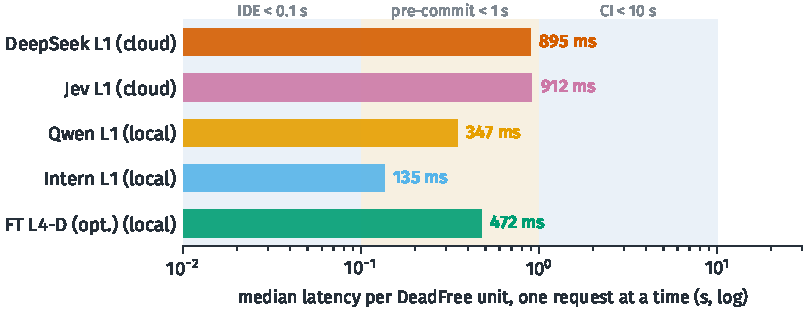
\includegraphics[width=\linewidth,height=0.60\textheight,keepaspectratio]{figures/df_intro_time.pdf}\\[4pt]
  \begin{tabular}{@{}ccc@{}}
    IDE: $<$\,0.1\,s & \quad pre-commit: $<$\,1\,s & \quad CI: $<$\,10\,s \\
  \end{tabular}
  \vfill
  {\scriptsize Cloud: DeepSeek V4.1 Flash API, Jev decision API (network round-trip). Local: one RTX 3090 (24\,GB).
  Median per DeadFree unit, one request at a time, same client.\par}
\end{frame}

% ------------------------------------------------------------------------------
% src: figures/df_intro_quality.pdf <- juliet_full/analysis/deadfree/deadfree_quality.json (macro_f1, eval 2,656 units)
\begin{frame}{On DeadFree, cloud models are far ahead of local ones}
  \centering
  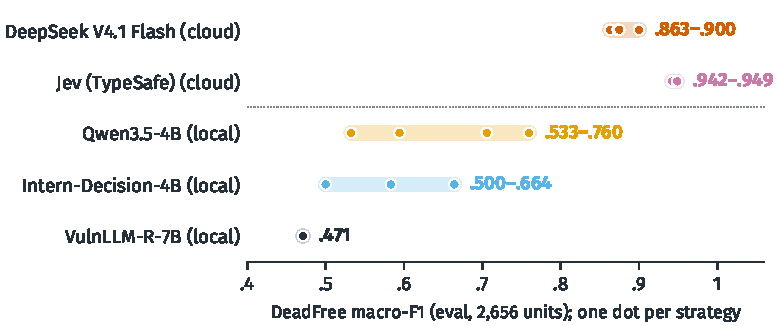
\includegraphics[width=\linewidth,height=0.60\textheight,keepaspectratio]{figures/df_intro_quality.pdf}\\[4pt]
  {\small Cloud \res{df-deepseek_L1}{macro}--\res{df-jev_L3}{macro};
  best untuned local prompt (L1--L4): Qwen L3 \res{df-qwen_L3}{macro}; VulnLLM-R-7B (vulnerability-tuned): \res{df-vulnllmr}{macro}\par}
  \vfill
  {\scriptsize DeadFree: Juliet CWE-401 units with a \code{free} that never runs (method section). Macro-F1, leak = positive class.\par}
\end{frame}

% ------------------------------------------------------------------------------
% src: figures/hook_original.pdf <- juliet_full/data/build/probes.json (static void) and registry runs on layer "original"
\begin{frame}{Original Juliet can be gamed: a one-line rule beats Clang SA}
  \begin{columns}[c]
    \begin{column}{0.57\textwidth}
      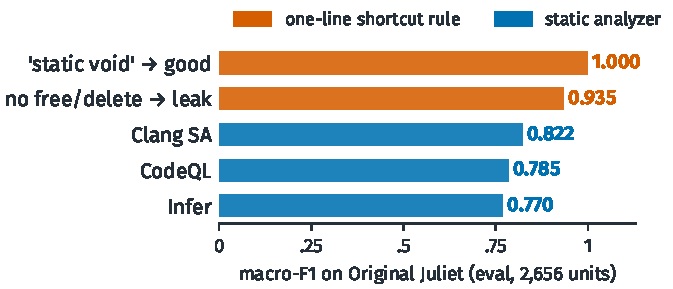
\includegraphics[width=\linewidth]{figures/hook_original.pdf}
    \end{column}
    \begin{column}{0.41\textwidth}
      \begin{itemize}
        \item ``no \code{free}/\code{delete} $\Rightarrow$ leak'': \res{grep-original}{macro}
        \item ``has \code{static void} $\Rightarrow$ good'': \res{x}{probe_static_void_original}
        \item Clang SA: \res{clang_sa-original}{macro}
      \end{itemize}
      \vspace{6pt}
      \alert{Templates reveal the label.}
    \end{column}
  \end{columns}
  \vfill
  {\scriptsize Template shortcuts: Germano et al.\ (ICAART'25); Risse \& B\"ohme (USENIX Sec'24).\par}
\end{frame}

% ------------------------------------------------------------------------------
\begin{frame}{Question: near-cloud quality on a local device?}
  \centering
  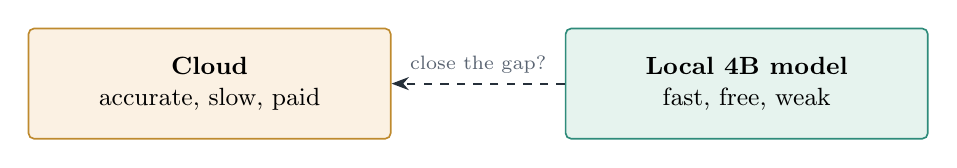
\begin{tikzpicture}[node distance=5mm and 8mm]
    \node[warn, minimum width=46mm, minimum height=14mm] (cloud) {\textbf{Cloud}\\{\small accurate, slow, paid}};
    \node[data, right=22mm of cloud, minimum width=46mm, minimum height=14mm] (local) {\textbf{Local 4B model}\\{\small fast, free, weak}};
    \draw[arr, dashed] (local.west) -- node[lbl, above] {close the gap?} (cloud.east);
  \end{tikzpicture}
  \vspace{10pt}
  \begin{enumerate}
    \item Which \textbf{strategy} helps a local model most?
    \item Does \textbf{fine-tuning} help, and on which labels?
    \item How close to the cloud do we get, and how fast?
  \end{enumerate}
  \vspace{4pt}
  {\small Task: one Juliet CWE-401 unit (C/C++) $\to$ leak / no leak, judged on \textbf{DeadFree}.\par}
\end{frame}

\section{Methods}

% ------------------------------------------------------------------------------
\begin{frame}{Debiased: good units now look like bad units}
  \centering
  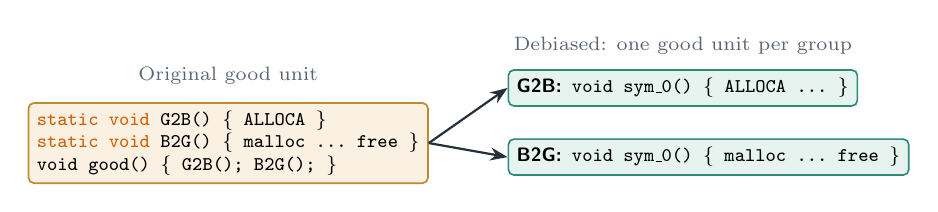
\begin{tikzpicture}[node distance=4mm and 10mm,
      codebox/.style={box, align=left, font=\ttfamily\scriptsize, inner sep=3pt}]
    \node[codebox, draw=WarnDraw, fill=WarnFill] (orig) {%
      \textcolor{OIvermil}{\textbf{static void}} G2B()\ \{ ALLOCA \}\\
      \textcolor{OIvermil}{\textbf{static void}} B2G()\ \{ malloc \dots\ free \}\\
      void good()\ \{ G2B(); B2G(); \}};
    \node[lbl, above=1mm of orig] {Original good unit};
    \node[codebox, draw=DataDraw, fill=DataFill, right=10mm of orig, yshift=7mm] (g2b) {%
      {\sffamily\bfseries G2B:}\ void sym\_0()\ \{ ALLOCA \dots\ \}};
    \node[codebox, draw=DataDraw, fill=DataFill, below=4mm of g2b.south west, anchor=north west] (b2g) {%
      {\sffamily\bfseries B2G:}\ void sym\_0()\ \{ malloc \dots\ free \}};
    \node[lbl] at ($(g2b.north)+(0,3mm)$) {Debiased: one good unit per group};
    \draw[arr] (orig.east) -- (g2b.west);
    \draw[arr] (orig.east) -- (b2g.west);
  \end{tikzpicture}
  \vspace{6pt}
  \begin{itemize}
    \item One entry function; wrapper and \code{static} removed
    \item Good unit is either G2B (no heap) or B2G (malloc + free)
    \item Bad units unchanged; same shape and length
  \end{itemize}
\end{frame}

% ------------------------------------------------------------------------------
\begin{frame}[fragile]{DeadFree adds a \code{free} that never runs}
  \begin{columns}[T]
    \begin{column}{0.48\textwidth}
      \textbf{bad} + dead free $\Rightarrow$ still \alert{leak}
\begin{lstlisting}[style=unit]
static const int sym_7 = 5;
data = (char *)malloc(100);
(*\hlc{if (sym\_7 != 5) \{ free(data); \}}*)
\end{lstlisting}
      \textbf{good}: real free, always-true guard
\begin{lstlisting}[style=unit]
(*\hlc{if (sym\_7 == 5) \{ free(data); \}}*)
\end{lstlisting}
    \end{column}
    \begin{column}{0.48\textwidth}
      \textbf{Placebo} (control): same guard, no free
\begin{lstlisting}[style=unit]
if (sym_7 != 5) { printLine("..."); }
\end{lstlisting}
      \vspace{4pt}
      \begin{itemize}
        \item Labels do not change
        \item Both labels now contain a \code{free}
        \item Only path feasibility decides
      \end{itemize}
    \end{column}
  \end{columns}
  \vfill
  {\scriptsize Dead frees in both labels; G2B goods get one too. All 3,316 units per layer compile (gcc, clang); labels re-checked by running them.\par}
\end{frame}

% ------------------------------------------------------------------------------
% src: fold sizes juliet_full/data/build/layer3.jsonl (set=eval: fold0 15 variants/472 groups, fold1 12/424, fold2 12/432)
\begin{frame}{We test on unseen flow variants}
  \centering
  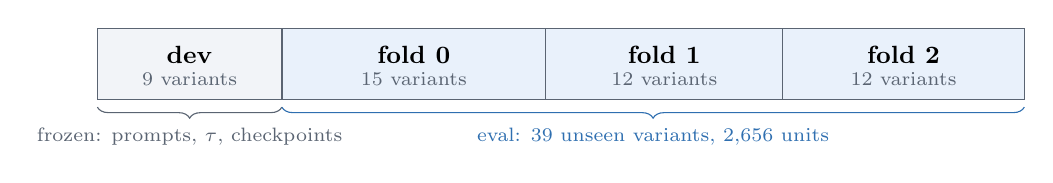
\begin{tikzpicture}[x=0.071mm, y=1mm]
    % widths proportional to groups: dev 330, fold0 472, fold1 424, fold2 432 (total 1,658)
    \foreach \x/\w/\c/\name/\sub in {0/330/NeutFill/dev/9 variants, 330/472/HeroFill/fold 0/15 variants,
        802/424/HeroFill/fold 1/12 variants, 1226/432/HeroFill/fold 2/12 variants}{
      \fill[\c, draw=NeutDraw, line width=0.5pt] (\x,0) rectangle ++(\w,9);
      \node[font=\small] at (\x+\w/2,5.6) {\textbf{\name}};
      \node[font=\scriptsize, text=NeutDraw] at (\x+\w/2,2.6) {\sub};
    }
    \draw[decorate, decoration={brace, amplitude=4pt, mirror}, NeutDraw] (0,-1) -- (330,-1)
      node[midway, below=4pt, lbl] {frozen: prompts, $\tau$, checkpoints};
    \draw[decorate, decoration={brace, amplitude=4pt, mirror}, HeroDraw] (330,-1) -- (1658,-1)
      node[midway, below=4pt, lbl, text=HeroDraw] {eval: 39 unseen variants, 2,656 units};
  \end{tikzpicture}
  \vspace{8pt}
  \begin{itemize}
    \item Split by Juliet flow variant, not by unit
    \item Fine-tuning: train on two folds, predict the third
    \item Macro-F1 (leak = positive), family-cluster bootstrap CI
    \item Speed: median latency per unit, one request at a time
  \end{itemize}
\end{frame}

% ------------------------------------------------------------------------------
\begin{frame}{L1--L3: ask for the verdict, with more or less help}
  \centering
  \renewcommand{\arraystretch}{1.2}
  \begin{tabular}{@{}lll@{}}
    \toprule
    & Prompt input & Answer \\
    \midrule
    \textbf{L1} direct & unit code & leak / no leak \\
    \textbf{L2} few-shot & + fixed dev examples & leak / no leak \\
    \textbf{L3} analysis-guided & + Clang SA warnings as evidence & leak / no leak \\
    \bottomrule
  \end{tabular}
  \vspace{10pt}
  \begin{columns}[T]
    \begin{column}{0.47\textwidth}
      \textbf{Generative} model\\
      {\small writes the label as JSON\\DeepSeek, Qwen3.5-4B, VulnLLM-R}
    \end{column}
    \begin{column}{0.47\textwidth}
      \textbf{Decision} model\\
      {\small one forward pass, reads P(Yes) vs P(No)\\Jev, Intern-Decision-4B, ours}
    \end{column}
  \end{columns}
  \vfill
  {\scriptsize Same prompt text for every model (VulnLLM-R: its authors' prompt); temperature 0, thinking off; prompts frozen on dev.\par}
\end{frame}

% ------------------------------------------------------------------------------
% src: L4 = juliet_full/llm/l4/leak.dl (v3); L4-D = juliet_full/l4d/README.md (contract), juliet_full/l4d/l4d.dl,
%   question templates juliet_full/l4d/templates.py
\begin{frame}{L4 and L4-D: the model supplies facts, Datalog decides}
  \centering
  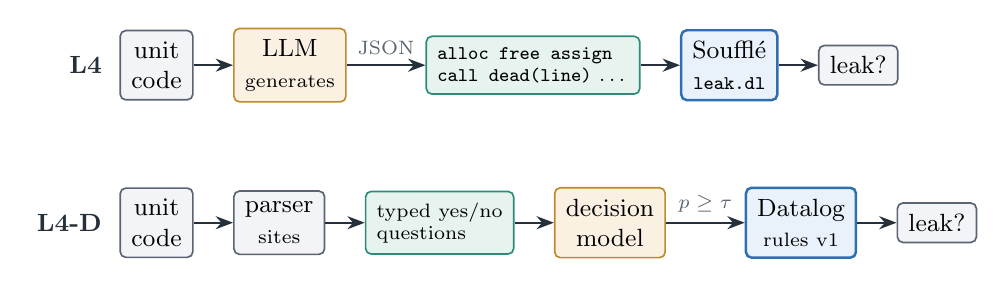
\begin{tikzpicture}[node distance=3mm and 5mm]
    % L4
    \node[box] (c1) {unit\\code};
    \node[warn, right=of c1] (llm) {LLM\\{\scriptsize generates}};
    \node[data, right=10mm of llm, font=\scriptsize, align=left] (f1) {\texttt{alloc free assign}\\\texttt{call dead(line)} \dots};
    \node[hero, right=of f1] (dl1) {Souffl\'e\\{\scriptsize \texttt{leak.dl}}};
    \node[box, right=of dl1] (o1) {leak?};
    \node[lbl, left=1mm of c1, font=\small\bfseries, text=Ink] {L4};
    \draw[arr] (c1) -- (llm); \draw[arr] (llm) -- node[lbl, above] {JSON} (f1); \draw[arr] (f1) -- (dl1); \draw[arr] (dl1) -- (o1);
    % L4-D
    \node[box, below=11mm of c1] (c2) {unit\\code};
    \node[box, right=of c2] (sites) {parser\\{\scriptsize sites}};
    \node[data, right=of sites, align=left, font=\scriptsize] (q) {typed yes/no\\questions};
    \node[warn, right=of q] (dm) {decision\\model};
    \node[hero, right=10mm of dm] (dl2) {Datalog\\{\scriptsize rules v1}};
    \node[box, right=of dl2] (o2) {leak?};
    \node[lbl, left=1mm of c2, font=\small\bfseries, text=Ink] {L4-D};
    \draw[arr] (c2) -- (sites); \draw[arr] (sites) -- (q); \draw[arr] (q) -- (dm);
    \draw[arr] (dm) -- node[lbl, above] {$p\geq\tau$} (dl2); \draw[arr] (dl2) -- (o2);
  \end{tikzpicture}
  \vspace{6pt}

  {\small
  \begin{tabular}{@{}ll@{}}
    \code{heap(a)} & Does the call at line $a$ allocate heap memory? \\
    \code{exec\_any(s)} & Can the (masked) statement $s$ run on \emph{at least one} run? \\
    \code{exec\_all(s)} & Does $s$ run on \emph{every} run? \\
    \code{rel(f,a)} & Does the release at $f$ free the block from $a$? \\
    \code{realloc\_safe(r)} & If \code{realloc} at $r$ fails, is the old block still released? \\
  \end{tabular}\par}
\end{frame}

% ------------------------------------------------------------------------------
% src: juliet_full/l4d/l4d.dl (rules v1, verbatim modulo the unit argument)
\begin{frame}[fragile]{Three rules turn the answers into a verdict}
  \begin{columns}[c]
    \begin{column}{0.56\textwidth}
\begin{lstlisting}[style=dl]
freed(a) :- rel(f, a), exec_all(f).
leak(a)  :- heap(a), exec_any(a), !freed(a).
leak(a)  :- realloc(a), exec_any(a),
            !realloc_safe(a).
unit_leak :- leak(_).
\end{lstlisting}
    \end{column}
    \begin{column}{0.42\textwidth}
      \begin{itemize}
        \item A leak: \emph{may} be allocated, \emph{not must} be freed
        \item The dead free fails \code{exec\_all}
        \item The model answers small local questions, not the whole verdict
      \end{itemize}
    \end{column}
  \end{columns}
  \vspace{8pt}
  {\small Facts: \code{heap}, \code{exec\_any}, \code{exec\_all}, \code{rel}, \code{realloc\_safe} from the model;
  site lists (\code{realloc}) from the parser. Run by Souffl\'e; a Python twin agrees on every unit.\par}
\end{frame}

% ------------------------------------------------------------------------------
% src (lectures, verified with pdftotext 2026-11-24 in /home/barton/Documents/projects/cs224/slides/):
%   Lecture 10 "Pointer Analysis": "Allocation-Site Abstraction ... one abstract object per allocation site";
%     analysis scope "Demand-driven: only compute points-to information for the pointers that may affect specific sites of interest".
%   Lecture 3-4 "Data Flow Analysis": "may analysis ... over-approximation; must analysis ... under-approximation";
%     Reaching Definitions (may), Available Expressions (must).
%   Lecture 17 "Datalog-Based Program Analysis": EDB/IDB predicates, negation !B(...), pointer/taint analysis via Datalog.
%   Lecture 1 "Introduction" (sound / complete); Lecture 18 "Soundiness": "Virtually all published whole-program
%     analyses are unsound when applied to real programming languages".
\begin{frame}{The design follows the course's program-analysis ideas}
  \small
  \renewcommand{\arraystretch}{1.15}
  \begin{tabular}{@{}p{0.36\linewidth}p{0.58\linewidth}@{}}
    \toprule
    L4-D element & Course idea (lecture) \\
    \midrule
    one fact set per \code{malloc}/\code{new} site & allocation-site abstraction (L10 Pointer Analysis) \\
    \code{exec\_any} / \code{exec\_all} & may vs must analysis, cf.\ reaching definitions vs available expressions (L3--4 Data Flow Analysis) \\
    \code{leak} = may-allocated $\wedge$ $\neg$must-freed & may/must safe approximation (L3--4) \\
    facts $\to$ rules with negation & Datalog-based program analysis: EDB, IDB, \code{!} (L17) \\
    ask only what \code{leak} needs & demand-driven analysis (L10) \\
    \midrule
    \textcolor{NeutDraw}{model facts can be wrong} & \textcolor{NeutDraw}{no soundness guarantee; real analyzers are ``soundy'' too (L1, L18)} \\
    \bottomrule
  \end{tabular}
\end{frame}

% ------------------------------------------------------------------------------
% src: juliet_full/l4d_ft/prune.py (needed()), juliet_full/l4d_ft/results/scores/prune_test.json
%   (questions_per_unit_eval medians; pred_diffs for gold and stored lora_l4d answers, all folds and layers)
\begin{frame}{Asking only what the rules read halves the questions}
  \centering
  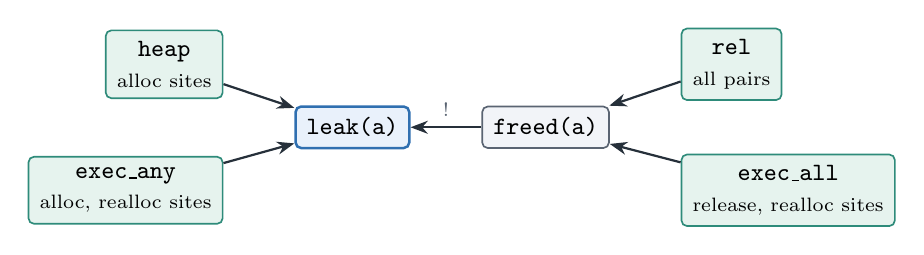
\begin{tikzpicture}[node distance=4mm and 9mm, every node/.style={font=\small}]
    \node[hero] (leak) {\code{leak(a)}};
    \node[data, left=of leak, yshift=8mm] (heap) {\code{heap}\\{\scriptsize alloc sites}};
    \node[data, left=of leak, yshift=-8mm] (any) {\code{exec\_any}\\{\scriptsize alloc, realloc sites}};
    \node[box, right=of leak] (freed) {\code{freed(a)}};
    \node[data, right=of freed, yshift=8mm] (rel) {\code{rel}\\{\scriptsize all pairs}};
    \node[data, right=of freed, yshift=-8mm] (all) {\code{exec\_all}\\{\scriptsize release, realloc sites}};
    \draw[arr] (heap) -- (leak); \draw[arr] (any) -- (leak);
    \draw[arr] (freed) -- node[lbl, above] {!} (leak);
    \draw[arr] (rel) -- (freed); \draw[arr] (all) -- (freed);
  \end{tikzpicture}
  \vspace{6pt}
  \begin{itemize}
    \item Backward from \code{leak}: drop facts no rule reads (e.g.\ \code{exec\_*} on plain statements)
    \item Median questions per DeadFree unit: \res{df-x}{q_full_layer3} $\to$ \alert{\res{df-x}{q_pruned_layer3}}
    \item Verdict differences on all 4 layers: \res{df-x}{prune_diffs_total}
  \end{itemize}
  \vfill
  {\scriptsize Optimized inference, post-hoc (user-approved 2026-11-24); same trained models, same $\tau$. ``L4-D (opt.)'' below.\par}
\end{frame}

% ------------------------------------------------------------------------------
% src: oracle and attribution = juliet_full/analysis/l4d_peek/fact_error_attribution.out.txt (gold facts substituted per
%   fact type, rules frozen, eval 2,656 units); oracle FP all variant-12 goods: juliet_full/l4d/REPORT_stage1.md
\begin{frame}{With correct facts the rules are near-perfect; \code{exec\_all} is the bottleneck}
  \begin{columns}[c]
    \begin{column}{0.58\textwidth}
      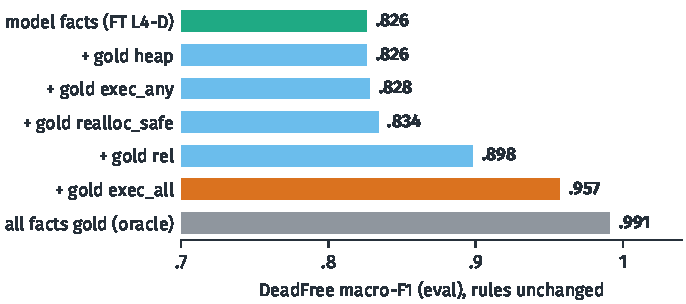
\includegraphics[width=\linewidth]{figures/df_attribution.pdf}
    \end{column}
    \begin{column}{0.40\textwidth}
      \begin{itemize}
        \item All gold facts: \res{df-x}{attr_layer3_all}, FN \res{df-x}{attr_layer3_all_fn}, FP \res{df-x}{attr_layer3_all_fp}
        \item Gold \code{exec\_all} only: \res{df-x}{attr_layer3_none} $\to$ \alert{\res{df-x}{attr_layer3_exec_all}}
        \item Errors come from wrong facts, mostly path feasibility
      \end{itemize}
    \end{column}
  \end{columns}
  \vfill
  {\scriptsize Gold facts from dynamic analysis. Oracle FPs: random-branch goods (flow variant 12) the path-insensitive rules cannot see.\par}
\end{frame}

% ------------------------------------------------------------------------------
% src: juliet_full/l4d/README.md (training contract), juliet_full/l4d_ft/PROGRESS.md (~68 min/fold, 2x RTX 3090 DDP),
%   decision_ft lane report (LoRA r16, 32.5 M trainable = 0.70 %)
\begin{frame}{Fine-tuning: one recipe, different labels per strategy}
  \centering
  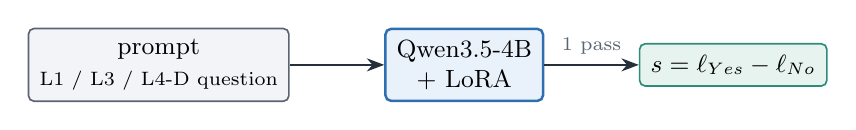
\begin{tikzpicture}[node distance=4mm and 12mm]
    \node[box, align=center] (in) {prompt\\{\scriptsize L1 / L3 / L4-D question}};
    \node[hero, right=of in, align=center] (m) {Qwen3.5-4B\\+ LoRA};
    \node[data, right=of m, align=center] (s) {$s=\ell_{\text{Yes}}-\ell_{\text{No}}$};
    \draw[arr] (in) -- (m); \draw[arr] (m) -- node[lbl, above] {1 pass} (s);
  \end{tikzpicture}
  \vspace{2pt}

  \small
  \renewcommand{\arraystretch}{1.1}
  \begin{tabular}{@{}lll@{}}
    \toprule
    Strategy & Training label & Loss \\
    \midrule
    L1, L3 & unit label (leak / no leak) & balanced CE + bad\,$>$\,good ranking \\
    L4-D & fact label from \textbf{dynamic analysis} & CE balanced per (question type, label) \\
    \bottomrule
  \end{tabular}
  \vspace{4pt}
  \begin{itemize}\small
    \item LoRA r16, $\alpha$32 on all LM linear layers: 32.5\,M weights (0.70\,\%); head from tied Yes/No rows
    \item Fact labels: gcov coverage, alloc/free trace, \code{realloc} failure injection; rules frozen
    \item 3-fold CV by flow variant; dev picks checkpoint and $\tau$; $\approx$68\,min/fold on 2$\times$ RTX 3090; L2 not trained
  \end{itemize}
\end{frame}

\section{Results}

% ------------------------------------------------------------------------------
% src: juliet_full/data/build/probes_layer3.json (eval split, macro-F1; BoW AUROC) via \res{df-x}{probe_*};
%   Clang SA from the registry runs (\res{clang_sa-<layer>}, \res{df-clang_sa}); G2B cue (ALLOCA / new):
%   juliet_full/lane_reports/2026-11-23_data_stage3.md:52
\begin{frame}{DeadFree removes the label shortcuts; one cue is left in G2B goods}
  \slidecite{\bib{clangsa}}
  \centering
  \renewcommand{\arraystretch}{1.15}
  \begin{tabular}{@{}lccc@{}}
    \toprule
    Shortcut probe (macro-F1) & Original & Debiased & DeadFree \\
    \midrule
    grep: no \code{free}/\code{delete} $\Rightarrow$ leak & \alert{\res{df-x}{probe_grep_v0_original}} & \res{df-x}{probe_grep_v0_layer1} & \res{df-x}{probe_grep_v0_layer3} \\
    \code{static void} $\Rightarrow$ good & \alert{\res{df-x}{probe_static_void_original}} & \res{df-x}{probe_static_void_layer1} & \res{df-x}{probe_static_void_layer3} \\
    bag-of-words logistic regression & \alert{\res{df-x}{probe_bow_lr_original}} & \res{df-x}{probe_bow_lr_layer1} & \res{df-x}{probe_bow_lr_layer3} \\
    \quad AUROC, B2G goods & \res{df-x}{probe_bow_auroc_B2G_original} & \res{df-x}{probe_bow_auroc_B2G_layer1} & \res{df-x}{probe_bow_auroc_B2G_layer3} \\
    \quad AUROC, G2B goods & \res{df-x}{probe_bow_auroc_G2B_original} & \res{df-x}{probe_bow_auroc_G2B_layer1} & \textcolor{OIvermil}{\res{df-x}{probe_bow_auroc_G2B_layer3}} \\
    \midrule
    \textcolor{NeutDraw}{Clang SA (reference)} & \textcolor{NeutDraw}{\res{clang_sa-original}{macro}} & \textcolor{NeutDraw}{\res{clang_sa-layer1}{macro}} & \textcolor{NeutDraw}{\res{df-clang_sa}{macro}} \\
    \bottomrule
  \end{tabular}
  \vspace{8pt}
  \begin{itemize}
    \item Residual: G2B goods still use \code{ALLOCA} or \code{new} instead of \code{malloc}
    \item \textbf{From here on, every model is compared on DeadFree only}
  \end{itemize}
\end{frame}

% ------------------------------------------------------------------------------
\begin{frame}{Two cloud services, three local models, one fine-tuned model}
  \slidecite{\bib{deepseekdocs}; \bib{deepseek2026v4}; \bib{typesafe2026jev}; \bib{qwen35card}; \bib{zhu2026interndecision}; \bib{nie2025vulnllmr}; \bib{hu2022lora}; \bib{clangsa}; \bib{inferpulse}; \bib{codeqldocs}; \bib{lsan}}
  \centering
  \footnotesize
  \renewcommand{\arraystretch}{1.05}
  \begin{tabular}{@{}llll@{}}
    \toprule
    Model & Where & Kind & Role \\
    \midrule
    DeepSeek V4.1 Flash & cloud API & generative & cloud reference (L1--L4) \\
    Jev (TypeSafe) & cloud API & decision & cloud reference (L1--L3, L4-D) \\
    \midrule
    Qwen3.5-4B & RTX 3090 & generative & LLM baseline \\
    Qwen read-out & RTX 3090 & decision (untuned) & starting point of our LoRA \\
    Intern-Decision-4B & RTX 3090 & decision & untuned decision baseline \\
    VulnLLM-R-7B & RTX 3090 & generative & vulnerability-tuned, published \\
    \textbf{ours}: Qwen3.5-4B + LoRA & RTX 3090 & decision & fine-tuned per strategy \\
    \midrule
    \textcolor{NeutDraw}{Clang SA, Infer, CodeQL, \dots} & \textcolor{NeutDraw}{CPU} & \textcolor{NeutDraw}{static} & \textcolor{NeutDraw}{tool reference} \\
    \textcolor{NeutDraw}{ASan/LSan, coverage + trace} & \textcolor{NeutDraw}{CPU} & \textcolor{NeutDraw}{dynamic} & \textcolor{NeutDraw}{runs the code} \\
    \bottomrule
  \end{tabular}
  \vfill
  {\scriptsize \textbf{Qwen read-out} = untuned Qwen3.5-4B used as a decision model: same yes/no question, read P(Yes) vs P(No) instead of letting it write. This is exactly our LoRA's starting point.\par}
\end{frame}

% ------------------------------------------------------------------------------
% src: figures/df_track_generative.tex, figures/df_track_decision.tex <- juliet_full/analysis/deadfree/deadfree_quality.json
%   (methods.json deadfree.tracks; bold = best cell per row, computed); jev_l4d prints "pending" until its row exists.
%   No L2 for read-out / FT: decided PLAN.md:35 (user, 2026-11-24 19:05: FT saw ~1,800 labelled units, L2 prompt 2.4x longer);
%   training units per fold 1,712-1,808: PLAN.md:110.
\begin{frame}{Two tracks $\times$ four strategies (DeadFree)}
  \slidecite{\bib{deepseekdocs}; \bib{typesafe2026jev}; \bib{qwen35card}; \bib{zhu2026interndecision}; \bib{hu2022lora}}
  \begin{columns}[T]
    \begin{column}{0.47\textwidth}
      {\small\textbf{Generative}: writes text, we parse it}\\[1pt]
      {\footnotesize\setlength{\tabcolsep}{3.5pt}% generated by figures/make_figures.py from juliet_full/analysis/deadfree/deadfree_quality.json
\begin{tabular}{@{}lcccc@{}}
\toprule
 & L1 & L2 & L3 & L4 \\
\midrule
Qwen3.5-4B & 0.533 & 0.595 & \textbf{0.760} & 0.706 \\
\midrule
DeepSeek (cloud) & 0.863 & 0.873 & 0.875 & \textbf{0.900} \\
\bottomrule
\end{tabular}
}
    \end{column}
    \begin{column}{0.51\textwidth}
      {\small\textbf{Decision}: one pass, read P(Yes) vs P(No)}\\[1pt]
      {\footnotesize\setlength{\tabcolsep}{3.5pt}% generated by figures/make_figures.py from juliet_full/analysis/deadfree/deadfree_quality.json
\begin{tabular}{@{}lcccc@{}}
\toprule
 & L1 & L2 & L3 & L4-D \\
\midrule
Qwen read-out & 0.351 & --$^\dagger$ & 0.334 & \textbf{0.752} \\
Intern-Decision & 0.584 & 0.500 & 0.664 & \textbf{0.799} \\
ours (LoRA) & 0.372 & --$^\dagger$ & 0.639 & \textbf{0.826} \\
\midrule
Jev (cloud) & 0.946 & 0.942 & \textbf{0.949} & 0.907 \\
\bottomrule
\end{tabular}
}
    \end{column}
  \end{columns}
  \footnotesize
  \begin{itemize}
    \item Cloud generative gains from writing facts (DeepSeek L4 \res{df-deepseek_L4}{macro}); the 4B model writes them poorly (L4 \res{df-qwen_L4}{macro} < L3 \res{df-qwen_L3}{macro})
    \item L4-D is the best strategy of every local decision model
    \item Same Qwen weights: \emph{asking} the facts (read-out L4-D \res{df-readout_l4d}{macro}) beats \emph{writing} them (gen.\ L4 \res{df-qwen_L4}{macro})
  \end{itemize}
  \vfill
  {\scriptsize Macro-F1; bold = best per row. Jev L4-D = cloud ceiling of the decision track.\\
  $^\dagger$Not run: FT already saw $\approx$1,800 labelled units; the L2 prompt is 2.4$\times$ longer.\par}
\end{frame}

% ------------------------------------------------------------------------------
% src: figures/df_before_after.pdf <- deadfree_quality.json strategy_x_ft (before: read-out = untuned Qwen3.5-4B weights;
%   after: lora_L1, lora_L3, lora_l4d_opt; marks: Intern-Decision, Qwen gen.); paired delta: deadfree_quality.json
%   paired_deltas; Debiased LoRA L1: registry lora_L1 layer1 (figures/numbers.tex \res{lora_L1-layer1})
\begin{frame}{FT: unit labels stay below the baselines, fact labels beat them}
  \slidecite{\bib{qwen35card}; \bib{hu2022lora}; \bib{zhu2026interndecision}; \bib{efron1979}}
  \centering
  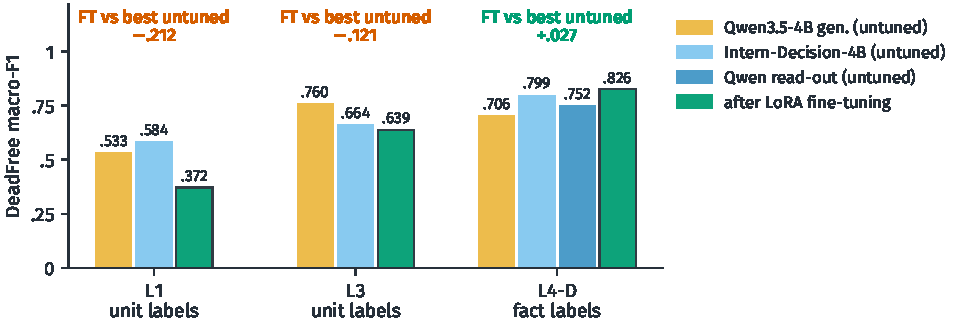
\includegraphics[width=\linewidth,height=0.46\textheight,keepaspectratio]{figures/df_before_after.pdf}\\[0pt]
  \raggedright\footnotesize
  \begin{itemize}
    \item L1/L3 learn \emph{unit labels} $\to$ the shortcut ``a \code{free} means no leak'': FT L1 scores \res{lora_L1-layer1}{macro} on Debiased, \alert{\res{df-lora_L1}{macro}} on DeadFree (leak recall \res{df-lora_L1}{r})
    \item L4-D learns \emph{fact labels} from dynamic analysis $\to$ transfers: \res{df-readout_l4d}{macro} $\to$ \textbf{\res{df-lora_l4d_opt}{macro}};
    vs untuned Intern L4-D \res{df-x}{pd_lora_l4d_opt__intern_l4d} \res{df-x}{pd_lora_l4d_opt__intern_l4d_ci}
  \end{itemize}
  \vfill
  {\scriptsize Same Qwen3.5-4B weights before (read-out) and after (LoRA). Intern-Decision at $\tau=0.5$. $\Delta$ CI: paired family-cluster bootstrap.\par}
\end{frame}

% ------------------------------------------------------------------------------
% src: figures/df_pareto.pdf <- deadfree_quality.json (macro_f1) x latency_deadfree.csv (median_s, log axis);
%   front over model-based methods; static tools grey; dynamic analysis dashed reference
\begin{frame}{FT L4-D is the most accurate local model, still below the cloud}
  \slidecite{\bib{deepseekdocs}; \bib{typesafe2026jev}; \bib{zhu2026interndecision}; \bib{nie2025vulnllmr}; \bib{clangsa}; \bib{inferpulse}; \bib{codeqldocs}; \bib{cppcheck}; \bib{serebryany2012asan}}
  \centering
  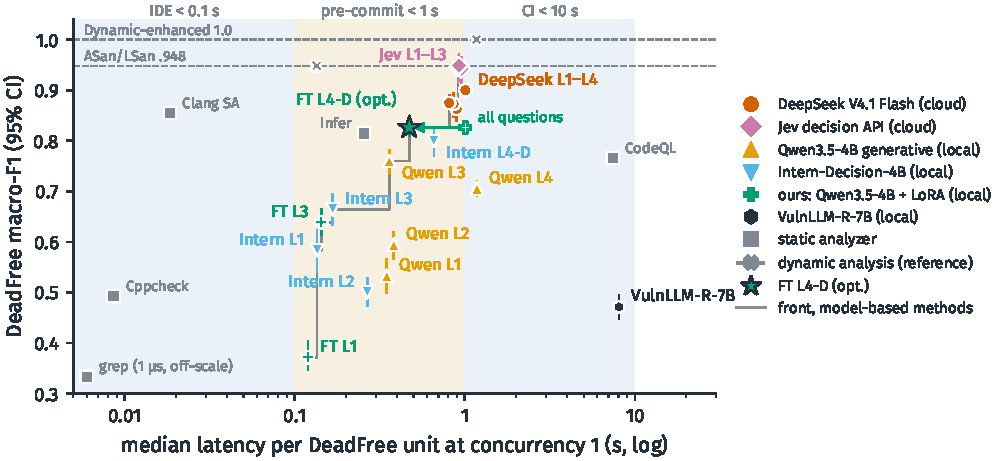
\includegraphics[width=\linewidth,height=0.70\textheight,keepaspectratio]{figures/df_pareto.pdf}
  \vfill
  {\scriptsize x: median latency per DeadFree unit, concurrency 1 (log); y: macro-F1 with 95\,\% CI.
  Shape = track, colour = cloud / local; grey: static tools; dashed: dynamic analysis (reference).\par}
\end{frame}

% ------------------------------------------------------------------------------
% src: deadfree_quality.json lora_l4d_opt / intern_l4d / clang_sa / jev_L3 / jev_l4d (pending until JEV_L4D_READY): delta_vs_ds_l1(_ci), gap_closed_ds_l1(_ci), delta_vs_ds_l4(_ci),
%   gap_closed_ds_l4(_ci); family-cluster bootstrap. Criterion pre-registered PLAN.md:224-226 (2026-11-23 22:30 PST,
%   before L4-D ran): near if macro-F1 point estimate >= reference - 0.02; reported as not met PLAN.md:34.
\begin{frame}{L4-D closes \res{df-intern_l4d}{gap1} of the gap untuned, \res{df-lora_l4d_opt}{gap1} fine-tuned; not near-cloud}
  \slidecite{\bib{deepseekdocs}; \bib{typesafe2026jev}; \bib{efron1979}}
  \centering
  \renewcommand{\arraystretch}{1.2}
  {\small
  \begin{tabular}{@{}llcc@{}}
    \toprule
    & vs & $\Delta$ macro-F1 [95\,\% CI] & gap closed \\
    \midrule
    Intern L4-D (untuned) & DeepSeek L1 (\res{df-deepseek_L1}{macro}) & \res{df-intern_l4d}{d1} \res{df-intern_l4d}{d1ci} & \res{df-intern_l4d}{gap1} \\
    \textbf{FT L4-D (opt.)} & DeepSeek L1 (\res{df-deepseek_L1}{macro}) & \res{df-lora_l4d_opt}{d1} \res{df-lora_l4d_opt}{d1ci} & \textbf{\res{df-lora_l4d_opt}{gap1}} \\
    \textbf{FT L4-D (opt.)} & DeepSeek L4 (\res{df-deepseek_L4}{macro}) & \res{df-lora_l4d_opt}{d4} \res{df-lora_l4d_opt}{d4ci} & \res{df-lora_l4d_opt}{gap4} \\
    \bottomrule
  \end{tabular}}\par
  \vspace{8pt}
  \begin{itemize}
    \item Gap measured from untuned Qwen L1 (\res{df-qwen_L1}{macro}) to the cloud model
    \item Criterion: $\geq$ reference $- 0.02$. \alert{Not met}: \res{df-lora_l4d_opt}{d1} vs DeepSeek L1
    \item Median latency: FT L4-D \res{df-lora_l4d_opt}{lat}, Intern L4-D \res{df-intern_l4d}{lat}, DeepSeek L1 \res{df-deepseek_L1}{lat} (FT L4-D \res{df-x}{speedup_ds_l1}$\times$ faster)
    \item Decision-track cloud ceiling: Jev L3 \res{df-jev_L3}{macro}, Jev L4-D \res{df-jev_l4d}{macro}
  \end{itemize}
\end{frame}

% ------------------------------------------------------------------------------
% src: figures/demo.tex <- presentation/demo/recordings/<newest stage_final*.json>; L4-D row from the frozen eval run
%   (juliet_full/l4d_ft/results/lora_l4d_opt/{layer1,layer3}/eval_r1_units.jsonl) until stage_final_v2 exists;
%   exec_all(free at line 20) p_yes 1.8e-07: juliet_full/l4d_ft/results/lora_l4d/layer3/eval_r1.jsonl
%   qid layer3/CWE401_Memory_Leak__strdup_char_01__bad/exec_all/s02
\begin{frame}[fragile]{Live: one dead free fools grep and the old LoRA, not L4-D}
  \slidecite{\bib{clangsa}; \bib{deepseekdocs}; \bib{typesafe2026jev}}
  \begin{columns}[T]
    \begin{column}{0.50\textwidth}
      {\small Bad unit \texttt{strdup\_char\_01}, DeadFree version:\par}
\begin{lstlisting}[style=unit]
static const int sym_61 = 4;
...
data = strdup(myString);
printLine(data);
(*\hlc{if(sym\_61 > 4) \{ free(data); \}}*)
\end{lstlisting}
      {\small The free never runs: still a leak.\par}
    \end{column}
    \begin{column}{0.48\textwidth}
      \textcolor{OIvermil}{\textbf{Flips to ``no leak''}}\\
      {\small \res{x}{demo_flipped}\par}
      \vspace{6pt}
      \textcolor{OIblue}{\textbf{Still ``leak''}}\\
      {\small \res{x}{demo_held}\par}
      \vspace{6pt}
      {\small L4-D: \code{exec\_all(free)} = no $\Rightarrow$ not freed $\Rightarrow$ leak\par}
    \end{column}
  \end{columns}
  \vfill
  {\scriptsize Full table in backup. Recording: \texttt{demo/recordings/\res{x}{demo_file}}; L4-D row: \res{x}{demo_has_l4d}.\par}
\end{frame}

\section{Discussion}

% ------------------------------------------------------------------------------
% src: deadfree_quality.json (macro_f1; lora_l4d_opt delta/gap); fact attribution
%   juliet_full/analysis/l4d_peek/fact_error_attribution.out.txt
\begin{frame}{Take-aways: what to fine-tune matters more than whether}
  \begin{enumerate}
    \item \textbf{Check the benchmark first.} On Original Juliet, grep scores \res{df-x}{probe_grep_v0_original}; on DeadFree \res{df-x}{probe_grep_v0_layer3}.
    \item \textbf{Unit labels teach shortcuts.} FT L1 drops to \res{df-lora_L1}{macro}, below both untuned baselines.
    \item \textbf{Fact labels transfer.} FT L4-D reaches \res{df-lora_l4d_opt}{macro}, the best local result.
    \item \textbf{Ask only what the rules read.} \res{df-x}{q_full_layer3} $\to$ \res{df-x}{q_pruned_layer3} questions, same verdicts.
    \item \textbf{Remaining gap = path feasibility.} Correct \code{exec\_all} alone gives \res{df-x}{attr_layer3_exec_all}.
  \end{enumerate}
\end{frame}

% ------------------------------------------------------------------------------
% src: Clang SA DeadFree quality deadfree_quality.json clang_sa (macro, delta_vs_ds_l1); latency latency_deadfree.csv
\begin{frame}{Limitations}
  \begin{itemize}
    \item \textbf{Clang SA is as good and faster}: \res{df-clang_sa}{macro} at \res{df-clang_sa}{lat}, no GPU. Path-sensitive analysis still matters
    \item \textbf{Synthetic data}: Juliet is public and templated; constant-guard dead frees are one kind of edit
    \item \textbf{Post-hoc pruning}: chosen after the full run; verdicts identical, approved 2026-11-24
    \item \textbf{$\tau$ and checkpoints}: dev is near-saturated, so selection is weakly informed
    \item \textbf{One local device}: one RTX 3090; other hardware will shift latency
    \item \textbf{Pending}: Intern-Decision L4-D; all DeadFree latencies fill in automatically
  \end{itemize}
\end{frame}

% ------------------------------------------------------------------------------
\begin{frame}[standout]
  Near-cloud quality on a local device?\\[6pt]
  \textbf{Close (\res{df-lora_l4d_opt}{gap1} of the gap), not yet near-cloud.}\\[14pt]
  {\normalsize Fine-tune on program-analysis facts, not on verdicts.}\\[18pt]
  Questions?
\end{frame}


\appendix
% Backup slides (after \appendix, not counted in the talk).

% ------------------------------------------------------------------------------
\begin{frame}[fragile]{Backup: where the template shortcut comes from}
  \begin{columns}[T]
    \begin{column}{0.42\textwidth}
      \textbf{bad unit}\\[1pt]
\begin{lstlisting}[style=unit]
void sym_0() {
  char *data = NULL;
  data = (char *)malloc(100);
  if (data == NULL) exit(-1);
  strcpy(data, "A String");
  printLine(data);
  ;                  /* no free */
}
\end{lstlisting}
      {\small Function names renamed to \texttt{sym\_N}; abridged.}
    \end{column}
    \begin{column}{0.54\textwidth}
      \textbf{good unit (Original)}\\[1pt]
\begin{lstlisting}[style=unit]
(*\hlc{static void}*) sym_1() {        /* G2B */
  char *data = (char *)ALLOCA(100);
  strcpy(data, "A String"); printLine(data);
}
(*\hlc{static void}*) sym_2() {        /* B2G */
  char *data = (char *)malloc(100);
  ...; printLine(data); free(data);
}
void sym_0() { sym_1(); sym_2(); }
\end{lstlisting}
      {\small Length, function count and \code{static} reveal the label.}
    \end{column}
  \end{columns}
\end{frame}

% ------------------------------------------------------------------------------
\begin{frame}{Backup: task and data}
  \begin{itemize}
    \item One Juliet\sref{sardjuliet13} CWE-401\sref{mitrecwe401} unit (C or C++) $\to$ leak / no leak
    \item 1,658 bad/good groups, 42 families, 48 flow variants
    \item C 868 / C++ 790 groups; 3,316 units per layer
    \item Debiased G2B / B2G good units $\approx$ 50/50 per flow category
    \item Dev 330 groups (9 variants); eval 1,328 groups (39 variants)
  \end{itemize}
\end{frame}

% ------------------------------------------------------------------------------
\begin{frame}{Backup: Original vs Debiased, all detectors}
  \centering
  {\footnotesize\renewcommand{\arraystretch}{0.82}% generated by figures/make_figures.py -- do not edit
\begin{tabular}{@{}lrr@{}}
\toprule
Detector & Original & Debiased \\
\midrule
\alert{\code{static void} $\Rightarrow$ good (probe)} & \alert{1.000} & \alert{0.333} \\
DeepSeek L1 & 0.961$^\dagger$ & 0.995 \\
Jev L1 & 0.956 & 0.971 \\
\textcolor{NeutDraw}{ASan/LSan (ref.)} & \textcolor{NeutDraw}{0.945} & \textcolor{NeutDraw}{0.945} \\
LoRA decision model L1 & 0.943 & 0.984 \\
\alert{grep: no \code{free}/\code{delete} $\Rightarrow$ leak} & \alert{0.935} & \alert{0.701} \\
Clang SA & 0.822 & 0.855 \\
CodeQL & 0.785 & 0.882 \\
Infer & 0.770 & 0.815 \\
Intern-Decision L1 & 0.642 & 0.825 \\
Qwen3.5-4B L1 & 0.572 & 0.754 \\
Cppcheck & 0.467 & 0.493 \\
LineVul & 0.356 & 0.501 \\
\bottomrule
\end{tabular}
}\\[2pt]
  {\scriptsize Macro-F1 on the eval set (2,656 units). $^\dagger$\,DeepSeek: nested25 subset (664 units).
  Tools: Clang SA\sref{clangsa}, Infer\sref{inferpulse}, CodeQL\sref{codeqldocs}, Cppcheck\sref{cppcheck}, LSan\sref{lsan}, LineVul\sref{fu2022linevul}.\par}
\end{frame}

% ------------------------------------------------------------------------------
% src: figures/nearllm.pdf (Debiased eval, v3 figure); bootstrap juliet_full/analysis/near_llm_bootstrap.py
%   (seed 20261123, B=2000): LoRA L1 - DeepSeek L1 = -0.0113 [-0.0143, -0.0084]; latencies figures/latency_c1.csv
%   (Debiased latency300, quiet re-measure); L4-D (opt.) Debiased 0.214 s: juliet_full/l4d_ft/REPORT_stage1.md:137
%   (fallback kernel = prediction config)
\begin{frame}{Backup: on Debiased, the unit-label LoRA was near-cloud}
  \begin{columns}[c]
    \begin{column}{0.58\textwidth}
      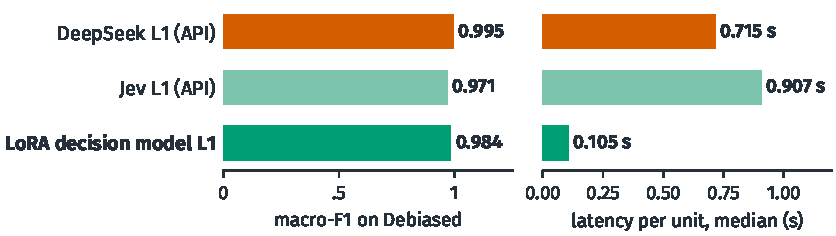
\includegraphics[width=\linewidth]{figures/nearllm.pdf}
    \end{column}
    \begin{column}{0.40\textwidth}
      \small
      \begin{itemize}
        \item LoRA L1 \res{lora_L1-layer1}{macro} vs DeepSeek L1 \res{deepseek_L1-layer1}{macro}: $\Delta$ $-0.011$ $[-0.014, -0.008]$
        \item Debiased latency: 0.105\,s vs 0.715\,s ($\approx$7$\times$)
        \item Same model on DeadFree: \res{df-lora_L1}{macro}
      \end{itemize}
      \vspace{4pt}
      {\scriptsize Debiased latencies (concurrency 1): Clang\sref{clangsa} 0.018, LoRA L1 0.105, Intern\sref{zhu2026interndecision} 0.132, L4-D (opt.) 0.214, Qwen\sref{qwen35card} 0.333, DeepSeek 0.715, Jev 0.907\,s.\par}
    \end{column}
  \end{columns}
\end{frame}

% ------------------------------------------------------------------------------
% src: Debiased/Placebo from registry runs (\res{<key>-<layer>}); DeadFree from deadfree_quality.json (\res{df-<key>});
%   DeepSeek Placebo run is the nested25 subset (664 units)
\begin{frame}{Backup: Placebo control: the guard alone does not hurt}
  \centering
  \small
  \renewcommand{\arraystretch}{1.1}
  \begin{tabular}{@{}lccc@{}}
    \toprule
    Method & Debiased & Placebo (guard, no free) & DeadFree (dead free) \\
    \midrule
    DeepSeek L1 & \res{deepseek_L1-layer1}{macro} & \res{deepseek_L1-placebo}{macro}$^\dagger$ & \res{df-deepseek_L1}{macro} \\
    Jev L3 & \res{jev_L3-layer1}{macro} & \res{jev_L3-placebo}{macro} & \res{df-jev_L3}{macro} \\
    Qwen3.5-4B\sref{qwen35card} L3 & \res{qwen_L3-layer1}{macro} & \res{qwen_L3-placebo}{macro} & \res{df-qwen_L3}{macro} \\
    Intern-Decision\sref{zhu2026interndecision} L3 & \res{intern_L3-layer1}{macro} & \res{intern_L3-placebo}{macro} & \res{df-intern_L3}{macro} \\
    FT L1 (unit labels) & \res{lora_L1-layer1}{macro} & \res{lora_L1-placebo}{macro} & \alert{\res{df-lora_L1}{macro}} \\
    FT L3 (unit labels) & \res{lora_L3-layer1}{macro} & \res{lora_L3-placebo}{macro} & \alert{\res{df-lora_L3}{macro}} \\
    FT L4-D (opt.) & \res{lora_l4d_opt-layer1}{macro} & \res{lora_l4d_opt-placebo}{macro} & \res{df-lora_l4d_opt}{macro} \\
    Clang SA\sref{clangsa} & \res{clang_sa-layer1}{macro} & \res{clang_sa-placebo}{macro} & \res{df-clang_sa}{macro} \\
    grep & \res{grep-layer1}{macro} & \res{grep-placebo}{macro} & \res{df-grep_v0}{macro} \\
    \bottomrule
  \end{tabular}
  \vfill
  {\scriptsize The drop comes from the dead \code{free}, not from the extra branch. $^\dagger$\,nested25 subset (664 units).\par}
\end{frame}

% ------------------------------------------------------------------------------
% src: McNemar rows from report/final_en/tables/res_mcnemar.tex (18 pre-registered tests, Holm);
%   bootstrap rows from juliet_full/analysis/near_llm_bootstrap.py (seed 20261123, B=2000, family-cluster, macro-F1 difference).
\begin{frame}{Backup: paired tests on Debiased (2,656 units)}
  \centering
  \small
  \begin{tabular}{@{}llr@{}}
    \toprule
    A vs B & statistic & result \\
    \midrule
    LoRA L1 vs DeepSeek L1 & $\Delta$macro-F1, 95\% CI & $-0.0113$ $[-0.0143, -0.0084]$ \\
    & only-right units & 12 vs 42 \\
    LoRA L1 vs Jev L1 & $\Delta$macro-F1, 95\% CI & $+0.0132$ $[+0.0029, +0.0282]$ \\
    Intern\sref{zhu2026interndecision} L1 vs Qwen\sref{qwen35card} L1 & $\Delta$macro-F1 & $+0.0711$ \\
    \midrule
    DeepSeek L1 vs DeepSeek L4 & McNemar $b$/$c$, $p_\text{Holm}$ & 63 / 12, $6.2{\times}10^{-8}$ \\
    DeepSeek L1 vs Qwen L1 & McNemar $b$/$c$, $p_\text{Holm}$ & 641 / 0, $9.4{\times}10^{-140}$ \\
    DeepSeek L2 vs CodeQL\sref{codeqldocs} & McNemar $b$/$c$, $p_\text{Holm}$ & 306 / 0, $5.7{\times}10^{-67}$ \\
    \bottomrule
  \end{tabular}
  \vfill
  {\scriptsize Bootstrap: 2,000 family-cluster resamples. McNemar\sref{mcnemar1947}: 18 pre-registered tests, Holm\sref{holm1979}-corrected.\par}
\end{frame}


% ------------------------------------------------------------------------------
% src: juliet_full/analysis/l4d_peek/fact_error_attribution.out.txt via \res{df-x}{attr_layer3_*}
%   (gold facts substituted per question type, rules v1 frozen, eval 2,656 DeadFree units)
\begin{frame}{Backup: fact attribution on DeadFree}
  \centering
  \small
  \renewcommand{\arraystretch}{1.1}
  \begin{tabular}{@{}lccc@{}}
    \toprule
    Gold facts substituted & macro-F1 & FP & FN \\
    \midrule
    none (FT L4-D answers) & \res{df-x}{attr_layer3_none} & \res{df-x}{attr_layer3_none_fp} & \res{df-x}{attr_layer3_none_fn} \\
    \code{heap} & \res{df-x}{attr_layer3_heap} & \res{df-x}{attr_layer3_heap_fp} & \res{df-x}{attr_layer3_heap_fn} \\
    \code{exec\_any} & \res{df-x}{attr_layer3_exec_any} & \res{df-x}{attr_layer3_exec_any_fp} & \res{df-x}{attr_layer3_exec_any_fn} \\
    \code{exec\_all} & \alert{\res{df-x}{attr_layer3_exec_all}} & \res{df-x}{attr_layer3_exec_all_fp} & \res{df-x}{attr_layer3_exec_all_fn} \\
    \code{exec\_any} + \code{exec\_all} & \res{df-x}{attr_layer3_exec_any_exec_all} & \res{df-x}{attr_layer3_exec_any_exec_all_fp} & \res{df-x}{attr_layer3_exec_any_exec_all_fn} \\
    \code{rel} & \res{df-x}{attr_layer3_rel} & \res{df-x}{attr_layer3_rel_fp} & \res{df-x}{attr_layer3_rel_fn} \\
    \code{realloc\_safe} & \res{df-x}{attr_layer3_realloc_safe} & \res{df-x}{attr_layer3_realloc_safe_fp} & \res{df-x}{attr_layer3_realloc_safe_fn} \\
    all (oracle) & \res{df-x}{attr_layer3_all} & \res{df-x}{attr_layer3_all_fp} & \res{df-x}{attr_layer3_all_fn} \\
    \bottomrule
  \end{tabular}
  \vfill
  {\scriptsize Gold \code{rel} removes FNs but not FPs; gold \code{exec\_all} removes both.\par}
\end{frame}

% ------------------------------------------------------------------------------
% src: oracle = \res{df-x}{attr_<layer>_all(_fp|_fn)}; FT = \res{df-x}{attr_<layer>_none}; Original oracle .985:
%   juliet_full/l4d/REPORT_stage1.md:91-97; FPs all flow-variant-12 goods REPORT_stage1.md:102-110
\begin{frame}{Backup: oracle: rules v1 with gold facts}
  \centering
  \small
  \renewcommand{\arraystretch}{1.1}
  \begin{tabular}{@{}lccc@{}}
    \toprule
    & Debiased & DeadFree & Placebo \\
    \midrule
    gold facts (oracle) & \res{df-x}{attr_layer1_all} & \res{df-x}{attr_layer3_all} & \res{df-x}{attr_placebo_all} \\
    \quad FP / FN & \res{df-x}{attr_layer1_all_fp} / \res{df-x}{attr_layer1_all_fn} & \res{df-x}{attr_layer3_all_fp} / \res{df-x}{attr_layer3_all_fn} & \res{df-x}{attr_placebo_all_fp} / \res{df-x}{attr_placebo_all_fn} \\
    FT L4-D answers & \res{df-x}{attr_layer1_none} & \res{df-x}{attr_layer3_none} & \res{df-x}{attr_placebo_none} \\
    \bottomrule
  \end{tabular}
  \vspace{8pt}
  \begin{itemize}
    \item Every oracle error is a false positive on a flow-variant-12 good unit
    \item Variant 12 frees in \emph{both} random branches: each \code{free} has \code{exec\_all} = no, so \code{freed} never fires
    \item ``Some free on every path'' is not expressible with per-statement facts: the ceiling of rules v1
  \end{itemize}
\end{frame}

% ------------------------------------------------------------------------------
% src: juliet_full/l4d_ft/results/scores/lora_l4d_opt_<layer>_eval_r1.json (per_fold, all_eval)
\begin{frame}{Backup: L4-D per held-out fold}
  \centering
  \renewcommand{\arraystretch}{1.1}
  \begin{tabular}{@{}lcccc@{}}
    \toprule
    Layer & fold 0 & fold 1 & fold 2 & pooled \\
    \midrule
    Debiased & \res{df-x}{l4d_layer1_fold0} & \res{df-x}{l4d_layer1_fold1} & \res{df-x}{l4d_layer1_fold2} & \res{df-x}{l4d_layer1} \\
    \textbf{DeadFree} & \res{df-x}{l4d_layer3_fold0} & \res{df-x}{l4d_layer3_fold1} & \res{df-x}{l4d_layer3_fold2} & \textbf{\res{df-x}{l4d_layer3}} \\
    Placebo & \res{df-x}{l4d_placebo_fold0} & \res{df-x}{l4d_placebo_fold1} & \res{df-x}{l4d_placebo_fold2} & \res{df-x}{l4d_placebo} \\
    Original & \res{df-x}{l4d_original_fold0} & \res{df-x}{l4d_original_fold1} & \res{df-x}{l4d_original_fold2} & \res{df-x}{l4d_original} \\
    \bottomrule
  \end{tabular}
  \vfill
  {\scriptsize Each fold's model was trained on the other two folds; checkpoint and $\tau$ chosen on dev and frozen before eval.\par}
\end{frame}

% ------------------------------------------------------------------------------
% src: figures/df_by_flow.tex <- deadfree_quality.json by_flow
\begin{frame}{Backup: DeadFree by flow category}
  \centering
  {\small\resizebox{\linewidth}{!}{% generated by figures/make_figures.py from juliet_full/analysis/deadfree/deadfree_quality.json
\begin{tabular}{@{}lccccc@{}}
\toprule
Method & 01 baseline & 02–22 control flow & 31–45 data flow & 51–68 cross-file & 71–84 C++ objects \\
\midrule
DeepSeek L1 & 0.856 & 0.828 & 0.900 & 0.902 & 0.868 \\
DeepSeek L4 & 0.904 & 0.885 & 0.921 & 0.949 & 0.836 \\
Jev L3 & 0.916 & 0.906 & 0.962 & 0.998 & 0.994 \\
Qwen L3 & 0.893 & 0.836 & 0.769 & 0.703 & 0.457 \\
Intern L3 & 0.748 & 0.612 & 0.657 & 0.776 & 0.605 \\
FT L1 & 0.467 & 0.402 & 0.343 & 0.333 & 0.333 \\
FT L4-D (opt.) & 0.869 & 0.823 & 0.843 & 0.848 & 0.770 \\
Clang SA & 0.904 & 0.868 & 0.827 & 0.923 & 0.691 \\
\bottomrule
\end{tabular}
}\par}
  \vfill
  {\scriptsize Macro-F1 per Juliet\sref{sardjuliet13} flow-variant group, DeadFree eval. FT L1 collapses everywhere; FT L4-D is weakest on C++ objects.\par}
\end{frame}

% ------------------------------------------------------------------------------
% src: figures/df_track_generative.tex, figures/df_track_decision.tex <- deadfree_quality.json (methods.json deadfree.tracks;
%   bold = best cell per row, computed); jev_l4d prints "pending" until its row exists. No L2 for read-out / FT: PLAN.md:35.
\begin{frame}{Backup: two tracks $\times$ four strategies, all numbers}
  \begin{columns}[T]
    \begin{column}{0.47\textwidth}
      {\small\textbf{Generative}: writes text, we parse it}\\[1pt]
      {\footnotesize\setlength{\tabcolsep}{3.5pt}% generated by figures/make_figures.py from juliet_full/analysis/deadfree/deadfree_quality.json
\begin{tabular}{@{}lcccc@{}}
\toprule
 & L1 & L2 & L3 & L4 \\
\midrule
Qwen3.5-4B & 0.533 & 0.595 & \textbf{0.760} & 0.706 \\
\midrule
DeepSeek (cloud) & 0.863 & 0.873 & 0.875 & \textbf{0.900} \\
\bottomrule
\end{tabular}
}
    \end{column}
    \begin{column}{0.51\textwidth}
      {\small\textbf{Decision}: one pass, read P(Yes) vs P(No)}\\[1pt]
      {\footnotesize\setlength{\tabcolsep}{3.5pt}% generated by figures/make_figures.py from juliet_full/analysis/deadfree/deadfree_quality.json
\begin{tabular}{@{}lcccc@{}}
\toprule
 & L1 & L2 & L3 & L4-D \\
\midrule
Qwen read-out & 0.351 & --$^\dagger$ & 0.334 & \textbf{0.752} \\
Intern-Decision & 0.584 & 0.500 & 0.664 & \textbf{0.799} \\
ours (LoRA) & 0.372 & --$^\dagger$ & 0.639 & \textbf{0.826} \\
\midrule
Jev (cloud) & 0.946 & 0.942 & \textbf{0.949} & 0.907 \\
\bottomrule
\end{tabular}
}
    \end{column}
  \end{columns}
  \vfill
  {\scriptsize DeadFree macro-F1; bold = best per row; Jev and Intern at $\tau=0.5$ for every strategy.
  $^\dagger$Not run: FT already saw $\approx$1,800 labelled units; the L2 prompt is 2.4$\times$ longer.\par}
\end{frame}

% ------------------------------------------------------------------------------
% src: figures/df_pareto_full.pdf (same data and front as the main Pareto, every point labelled)
\begin{frame}{Backup: DeadFree Pareto, every point labelled}
  \centering
  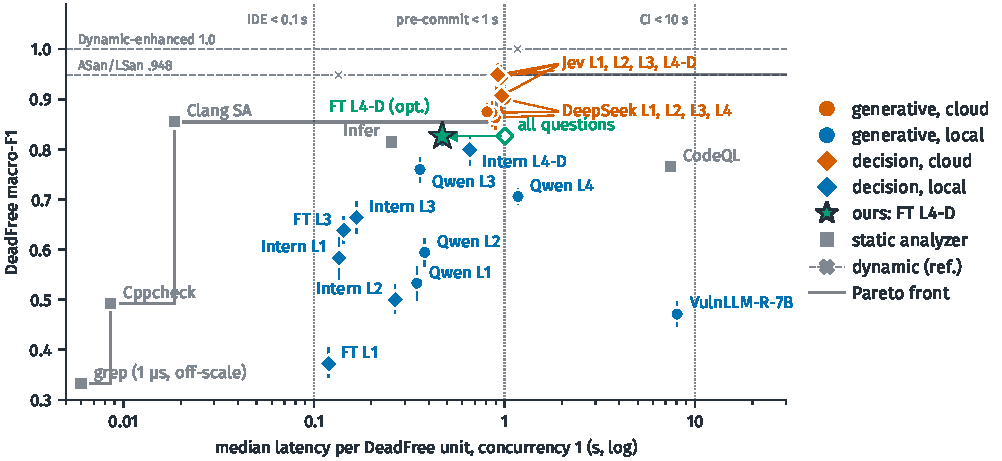
\includegraphics[width=\linewidth,height=0.72\textheight,keepaspectratio]{figures/df_pareto_full.pdf}
  \vfill
  {\scriptsize x: median latency per DeadFree unit, concurrency 1 (log); y: macro-F1 with 95\,\% CI. Front over model-based and static methods.\par}
\end{frame}

% ------------------------------------------------------------------------------
% src: figures/df_strategies.tex <- deadfree_quality.json strategy_x_ft + latency_deadfree.csv
\begin{frame}{Backup: strategy $\times$ local model, macro-F1 / median latency}
  \centering
  {\small\resizebox{\linewidth}{!}{% generated by figures/make_figures.py from juliet_full/analysis/deadfree (quality + latency)
\begin{tabular}{@{}lcccc@{}}
\toprule
Local model & L1 & L2 & L3 & L4 / L4-D \\
\midrule
Qwen3.5-4B (gen.) & 0.533 / {\scriptsize \textit{pending}} & 0.595 / {\scriptsize \textit{pending}} & 0.760 / {\scriptsize \textit{pending}} & 0.706 / {\scriptsize \textit{pending}} \\
Intern-Decision-4B & 0.584 / {\scriptsize \textit{pending}} & 0.500 / {\scriptsize \textit{pending}} & 0.664 / {\scriptsize \textit{pending}} & \textit{pending} / {\scriptsize \textit{pending}} \\
Qwen read-out (no FT) & -- & -- & -- & 0.752 / {\scriptsize \textit{pending}} \\
ours: Qwen3.5-4B + LoRA & 0.372 / {\scriptsize \textit{pending}} & -- & 0.639 / {\scriptsize \textit{pending}} & 0.826 / {\scriptsize 445\,ms} \\
\bottomrule
\end{tabular}
}\par}
  \vfill
  {\scriptsize DeadFree eval, 2,656 units; latency per unit at concurrency 1 on one RTX 3090; n/m = not measured.\par}
\end{frame}

% ------------------------------------------------------------------------------
% src: juliet_full/analysis/deadfree/deadfree_quality.json intern_l4d (tau 0.5, primary), intern_l4d_devtau
%   (dev tau 0.182426, secondary), readout_l4d, paired_deltas; notes[0] (switch after eval), notes[1] (failure)
\begin{frame}{Backup: Intern-Decision L4-D and its threshold}
  \centering
  \renewcommand{\arraystretch}{1.15}
  \begin{tabular}{@{}lcccc@{}}
    \toprule
    Intern-Decision-4B\sref{zhu2026interndecision}, L4-D & macro-F1 [95\,\% CI] & leak P & leak R & gap closed \\
    \midrule
    $\tau = 0.5$ (reported) & \res{df-intern_l4d}{macro} \res{df-intern_l4d}{ci} & \res{df-intern_l4d}{p} & \res{df-intern_l4d}{r} & \res{df-intern_l4d}{gap1} \\
    dev $\tau = 0.18$ (frozen) & \res{df-intern_l4d_devtau}{macro} \res{df-intern_l4d_devtau}{ci} & \res{df-intern_l4d_devtau}{p} & \res{df-intern_l4d_devtau}{r} & \res{df-intern_l4d_devtau}{gap1} \\
    \bottomrule
  \end{tabular}
  \vspace{6pt}
  \begin{itemize}\small
    \item \alert{Disclosure}: the primary was switched to $\tau=0.5$ after seeing eval, for consistency with Intern L1--L3; the switch favours the baseline
    \item Low dev $\tau$: every exec/release question is answered Yes (Intern's $p_{\text{yes}}$ lies in $\approx$0.45--0.65), so dead frees count as ``runs on every path''; a $\tau$ tuned on Debiased (no dead frees) does not transfer
    \item Paired: Intern L4-D $-$ Qwen read-out L4-D \res{df-x}{pd_intern_l4d__readout_l4d} \res{df-x}{pd_intern_l4d__readout_l4d_ci};\\ FT L4-D $-$ Intern L4-D \res{df-x}{pd_lora_l4d_opt__intern_l4d} \res{df-x}{pd_lora_l4d_opt__intern_l4d_ci}
  \end{itemize}
\end{frame}

% ------------------------------------------------------------------------------
% src: deadfree_quality.json jev_l4d (tau 0.5, pre-specified before any call, primary), jev_l4d_devtau (layer1-dev tau
%   0.268941, secondary), paired_deltas; fact accuracy, FP causes and latency protocol:
%   juliet_full/analysis/deadfree/REPORT_jev_l4d.md (eval table, "Reading", per-qtype table, latency table)
\begin{frame}{Backup: Jev L4-D, the cloud decision model on the same facts}
  \centering
  \renewcommand{\arraystretch}{1.15}
  \begin{tabular}{@{}lcccc@{}}
    \toprule
    Jev, L4-D & macro-F1 [95\,\% CI] & leak P & leak R & gap closed \\
    \midrule
    $\tau = 0.5$ (pre-specified) & \res{df-jev_l4d}{macro} \res{df-jev_l4d}{ci} & \res{df-jev_l4d}{p} & \res{df-jev_l4d}{r} & \res{df-jev_l4d}{gap1} \\
    dev-chosen $\tau = 0.27$ & \res{df-jev_l4d_devtau}{macro} \res{df-jev_l4d_devtau}{ci} & \res{df-jev_l4d_devtau}{p} & \res{df-jev_l4d_devtau}{r} & \res{df-jev_l4d_devtau}{gap1} \\
    \bottomrule
  \end{tabular}
  \vspace{6pt}
  \begin{itemize}\small
    \item Same pruned questions and rules as Intern and FT L4-D; $\tau = 0.5$ fixed before any Jev L4-D call
    \item Paired: vs DeepSeek L4 \res{df-x}{pd_jev_l4d__deepseek_L4} \res{df-x}{pd_jev_l4d__deepseek_L4_ci} (n.s.);
      vs Jev L3 \res{df-x}{pd_jev_l4d__jev_L3} \res{df-x}{pd_jev_l4d__jev_L3_ci};\\ vs FT L4-D \res{df-x}{pd_jev_l4d__lora_l4d_opt} \res{df-x}{pd_jev_l4d__lora_l4d_opt_ci}
    \item \code{exec\_all} fact accuracy 0.975 (FT L4-D 0.831): a strong decision model answers path questions well;
      most of its 238 false leaks contain a wrong \code{realloc\_safe} answer
    \item Latency \res{df-jev_l4d}{lat}: the questions of a unit are sent concurrently (local L4-D asks them one by one)
  \end{itemize}
\end{frame}

% ------------------------------------------------------------------------------
% src: deadfree_quality.json vulnllmr; configuration juliet_full/STATUS.md 2026-11-23 22:41 (authors' prompt with
%   policy hint CWE-401/1333/703/404, #judge: yes = leak, unparseable = wrong)
\begin{frame}{Backup: VulnLLM-R-7B, a vulnerability-reasoning model}
  \begin{itemize}
    \item VulnLLM-R-7B\sref{nie2025vulnllmr}: authors' prompt and policy hint (CWE-401, 1333, 703, 404); temperature 0
    \item DeadFree: macro-F1 \res{df-vulnllmr}{macro} \res{df-vulnllmr}{ci}
    \item Leak precision \res{df-vulnllmr}{p}, recall \res{df-vulnllmr}{r} (TP \res{df-vulnllmr}{tp}, FN \res{df-vulnllmr}{fn})
    \item Below both untuned 4B models on DeadFree
  \end{itemize}
  \vfill
  {\scriptsize ``\#judge: yes'' with any type = leak; unparseable or truncated output counts as wrong.\par}
\end{frame}

% ------------------------------------------------------------------------------
% src: prompts juliet_full/llm/prompts (frozen on dev); L4-D templates juliet_full/l4d/templates.py (TEMPLATE_SHA256,
%   frozen), abridged only by dropping the code snippet in backticks
\begin{frame}{Backup: prompts and the five L4-D question templates}
  \footnotesize
  \begin{description}[L4-D]
    \item[L1] unit code $\to$ \code{\{label, confidence\}}; decision models read P(leak)
    \item[L2] + fixed dev examples (few-shot)
    \item[L3] + Clang SA\sref{clangsa} warnings for the unit
    \item[L4] LLM lists \code{alloc/free/assign/call/dead(line)} facts as JSON; Souffl\'e\sref{jordan2016souffle} \code{leak.dl} decides
    \item[L4-D] one yes/no question per fact, statement under test masked as \code{\_\_TARGET\_\_();}
  \end{description}
  {\scriptsize
  \begin{tabular}{@{}lp{0.76\linewidth}@{}}
    \toprule
    \code{heap} & Does the call at line \{line\} allocate heap memory that the program must release? \\
    \code{exec\_any} & Can the statement at line \{line\} execute on at least one run of the program? \\
    \code{exec\_all} & Does the statement at line \{line\} execute on every run of the program? \\
    \code{rel} & Does the release at line \{line\_f\} free the block obtained at line \{line\_a\}? \\
    \code{realloc\_safe} & If the realloc at line \{line\} fails and returns NULL, is the original block still released later? \\
    \bottomrule
  \end{tabular}\par}
  \vfill
  {\scriptsize Same prompt text for all models; temperature 0, thinking off; frozen before eval.\par}
\end{frame}

% ------------------------------------------------------------------------------
% src: juliet_full/l4d/l4d.dl (rules v1, comments dropped)
\begin{frame}[fragile]{Backup: L4-D rules v1 (Souffl\'e, complete)}
\begin{lstlisting}[style=dl]
.input unit, alloc, realloc, heap, exec_any, exec_all, rel, realloc_safe
heap_block(u, a) :- alloc(u, a), heap(u, a).
heap_block(u, r) :- realloc(u, r).
freed(u, a) :- rel(u, f, a), exec_all(u, f).
leak(u, a, "never_freed")  :- heap_block(u, a), exec_any(u, a), !freed(u, a).
leak(u, r, "realloc_fail") :- realloc(u, r), exec_any(u, r), !realloc_safe(u, r).
unit_leak(u) :- leak(u, _, _).
.output leak, unit_leak
\end{lstlisting}
  \vspace{4pt}
  \begin{itemize}\small
    \item \code{alloc}, \code{realloc}: site lists from the tree-sitter\sref{url-treesitter} parser; all other inputs: model answers with $p \geq \tau$
    \item Frozen before training; refinements were allowed only from Debiased dev failures (there were none)
  \end{itemize}
\end{frame}

% ------------------------------------------------------------------------------
% src: juliet_full/llm/l4/leak.dl (v3 L4 rules, abridged); numbers from registry runs (DeepSeek DeadFree = nested25)
\begin{frame}[fragile]{Backup: L4 (LLM facts + Datalog), the v3 rule set}
  \begin{columns}[T]
    \begin{column}{0.59\textwidth}
\begin{lstlisting}[style=dl]
reach("main").
reach(g) :- reach(f), call(f, g, l), !dead(l).
new_obj(o, v, f) :- alloc(o, v, f, l),
                    reach(f), !dead(l).
pts(s, v, o) :- new_obj(o, v, f),
                scope(f, v, s).
pts(sd, d, o) :- assign(d, x, f, l), !dead(l),
                 ..., pts(sx, x, o).
freed(o) :- free(v, f, l), reach(f), !dead(l),
            ..., pts(s, v, o).
(*\textcolor{OIblue}{\bfseries leak(o, "never\_freed")}*) :-
        new_obj(o, _, _), !freed(o).
\end{lstlisting}
      {\tiny Abridged from \texttt{juliet\_full/llm/l4/leak.dl} (v3): Andersen-style, flow-insensitive;
      + \texttt{realloc\_fail} rule.\par}
    \end{column}
    \begin{column}{0.39\textwidth}
      \begin{itemize}\small
        \item DeepSeek L4, Debiased: \res{deepseek_L4-layer1}{macro} (L1 \res{deepseek_L1-layer1}{macro})
        \item DeadFree $\Delta$ \res{deepseek_L4-layer3}{d}, smallest of L1--L4 (L1 \res{deepseek_L1-layer3}{d})
        \item FP/FN: L1 \res{deepseek_L1-layer3}{fp}/\res{deepseek_L1-layer3}{fn},
              L4 \res{deepseek_L4-layer3}{fp}/\res{deepseek_L4-layer3}{fn}
        \item 99.87\% of facts grounded to a source line
        \item Qwen3.5-4B L4: \res{qwen_L4-layer1}{macro} $\to$ \res{qwen_L4-layer3}{macro}
      \end{itemize}
    \end{column}
  \end{columns}
  \vfill
  {\scriptsize Paired on nested25 (664 units). A dead \code{free} is dropped by \code{!dead(l)}, so the leak survives.\par}
\end{frame}


% ------------------------------------------------------------------------------
\begin{frame}{Backup: method matrix with versions}
  \footnotesize
  \renewcommand{\arraystretch}{0.9}
  \begin{tabular}{@{}lll@{}}
    \toprule
    Group & Method & Program-analysis idea \\
    \midrule
    Static & grep: is there a \code{free}/\code{delete}? & lexical baseline \\
           & Cppcheck\sref{cppcheck} 2.22 & intraprocedural dataflow \\
           & Clang SA\sref{clangsa} 23.1.6 & path-sensitive symbolic execution \\
           & CodeQL\sref{codeqldocs} 2.27.5 & Datalog-style queries over dataflow \\
           & Infer\sref{inferpulse} 1.3 (Pulse) & interprocedural summaries \\
    Generative & DeepSeek V4.1 Flash (API) $\times$ L1--L4 & L4: LLM facts + Datalog \\
        & Qwen3.5-4B (local) $\times$ L1--L4 & same prompts, one RTX 3090 \\
        & VulnLLM-R-7B\sref{nie2025vulnllmr} (local) & authors' reasoning prompt \\
    Decision & Jev (TypeSafe API) $\times$ L1--L3 & read the option probability \\
             & Intern-Decision-4B $\times$ L1--L3 (+ L4-D) & read the option probability \\
             & Qwen3.5-4B read-out $\times$ L4-D & untuned Yes/No head \\
             & \textbf{ours}: LoRA $\times$ \{L1, L3, L4-D\} & fine-tuned score, 3-fold CV \\
    \midrule
    \textcolor{NeutDraw}{Reference} & \textcolor{NeutDraw}{ASan/LSan\sref{lsan}, Valgrind\sref{nethercote2007valgrind}, Dynamic-enhanced} &
      \textcolor{NeutDraw}{runs the program: shown, not ranked} \\
    \bottomrule
  \end{tabular}
  \vfill
  {\scriptsize Missing output, timeout or compile error counts as a wrong prediction.\par}
\end{frame}

% ------------------------------------------------------------------------------
% src: figures/cost.tex <- juliet_full/llm/ledger.jsonl; per-1k cost report/final_en/generated/numbers.tex
%   (res-x-cost1k_deepseek_L1, res-x-cost1k_jev_L1); FT cost juliet_full/l4d_ft/PROGRESS.md:8
\begin{frame}{Backup: cost of every API run and of fine-tuning}
  \begin{columns}[T]
    \begin{column}{0.60\textwidth}
      {\scriptsize\resizebox{\linewidth}{!}{% generated by figures/make_figures.py from juliet_full/llm/ledger.jsonl
\begin{tabular}{@{}llrr@{}}
\toprule
Provider & Runs & calls & cost \\
\midrule
DeepSeek & Debiased (incl.\ dev, repeats, latency) & 13,877 & \textyen5.46 \\
DeepSeek & DeadFree & 11,824 & \textyen5.37 \\
DeepSeek & Placebo & 1,328 & \textyen0.42 \\
DeepSeek & Original & 664 & \textyen0.30 \\
DeepSeek & demo & 30 & \textyen0.01 \\
\textbf{DeepSeek} & \textbf{total} & \textbf{27,723} & \textbf{\textyen11.57} \\
\midrule
Jev & Debiased (incl.\ dev, repeats, latency) & 27,420 & \$1.23 \\
Jev & DeadFree & 8,868 & \$0.42 \\
Jev & Placebo & 5,312 & \$0.20 \\
Jev & Original & 2,656 & \$0.10 \\
Jev & demo & 11 & \$0.00 \\
\textbf{Jev} & \textbf{total} & \textbf{44,267} & \textbf{\$1.95} \\
\bottomrule
\end{tabular}
}\par}
    \end{column}
    \begin{column}{0.37\textwidth}
      \begin{itemize}\small
        \item Total: \textyen\res{x}{cost_deepseek} and \$\res{x}{cost_jev}
        \item Per 1k units: DeepSeek L1 \textyen0.397, Jev L1 \$0.0345
        \item L4-D fine-tuning: $\approx$68\,min per fold on 2$\times$ RTX 3090 ($\approx$2.3\,GPU-h)
        \item Local inference: no API cost
      \end{itemize}
    \end{column}
  \end{columns}
\end{frame}

% ------------------------------------------------------------------------------
\begin{frame}{Backup: Debiased latency at concurrency 1 (v3 measurements)}
  \centering
  {\tiny\renewcommand{\arraystretch}{0.92}\resizebox{\linewidth}{!}{% generated by figures/make_figures.py from figures/latency_c1.csv
\begin{tabular}{@{}lrl@{}}
\toprule
Method & s / unit & Source (juliet\_full/\ldots); note \\
\midrule
grep & <0.001 & \texttt{static/results/grep\_v0/layer1/lat300\_c1.jsonl}; median of 300 units (1 µs) \\
Cppcheck & 0.008 & \texttt{static\_stage2.md}; lat300 per unit \\
Clang SA & 0.018 & \texttt{static\_stage2.md}; lat300 per unit \\
Infer & 0.278 & \texttt{static\_stage2.md}; lat300 per unit \\
CodeQL & 7.36 & \texttt{static\_stage2.md}; per unit: database creation + queries (20 units) \\
CodeQL (50 per database) & 0.318 & \texttt{static\_stage2.md}; 50 units per database; amortized (hollow marker) \\
LineVul (GPU) & 0.006 & \texttt{gpu\_stage1.md}; GPU (RTX 3090) \\
LineVul (CPU) & 0.088 & \texttt{gpu/results/linevul\_cpu/layer1/lat300\_cpu\_quiet.jsonl}; CPU 6 threads; quiet; median of 300 \\
DeepSeek L1 & 0.721 & \texttt{llm\_stage2b.md}; lat300\_c1\_L1 at load ~21; quiet 0.640 s on 30 dev units (llm\_stage2a) \\
Qwen L1 & 0.665 & \texttt{gpu\_stage1.md}; vLLM from dell; 30 requests \\
Jev L1 & 0.961 & \texttt{llm\_stage2b.md}; lat300\_c1\_L1 at load ~22 \\
Intern-D L1 & 0.083 & \texttt{gpu\_stage1.md}; /decide read-out from dell (82.7 ms) \\
LoRA L1 & 0.105 & \texttt{decision\_ft\_stage2.md}; latency300; dell end-to-end \\
LoRA L3 & 0.133 & \texttt{decision\_ft\_stage2.md}; latency300; dell end-to-end \\
ASan/LSan & 0.134 & \texttt{data\_stage4.md}; lat300\_c1; compile included \\
Valgrind & 0.407 & \texttt{data\_stage4.md}; lat300\_c1; compile included \\
Dyn. enhanced & 1.194 & \texttt{data\_stage4.md}; lat300\_c1; compile included \\
\bottomrule
\end{tabular}
}\par}
  \vfill
  {\scriptsize Measured on \textbf{Debiased} units; the DeadFree latencies in the main slides are re-measured separately.
  Source table: \texttt{figures/latency\_c1.csv}.\par}
\end{frame}

% ------------------------------------------------------------------------------
\begin{frame}{Backup: are the labels still right? Compile and run every unit}
  \begin{columns}[T]
    \begin{column}{0.46\textwidth}
      \begin{itemize}\small
        \item gcc and clang compile \textbf{3,316 / 3,316} units in every layer
        \item No good unit flagged by ASan\sref{serebryany2012asan}/LSan\sref{lsan} or Dynamic-enhanced
        \item Labels never changed; disagreements explained
      \end{itemize}
    \end{column}
    \begin{column}{0.51\textwidth}
      {\footnotesize Dynamic-enhanced: what it takes to catch the 1,658 bad units\\[2pt]
      \begin{tabular}{@{}lr@{}}
        \toprule
        Needed & units \\
        \midrule
        plain run, every seed & 1,448 \\
        some seeds only (variant 12, random) & 34 \\
        \texttt{use\_globals=0} (globals at exit) & 68 \\
        \texttt{realloc} failure injected & 108 \\
        \bottomrule
      \end{tabular}}
    \end{column}
  \end{columns}
\end{frame}


% ------------------------------------------------------------------------------
% src: deadfree_quality.json asan_lsan / dynamic_enhanced; misses juliet_full/lane_reports data_stage4 (v3 backup)
\begin{frame}{Backup: dynamic analysis is a reference line, not a competitor}
  \begin{itemize}
    \item ASan\sref{serebryany2012asan}/LSan\sref{lsan} on DeadFree: precision \res{df-asan_lsan}{p}, macro-F1 \res{df-asan_lsan}{macro}
    \item Misses: \code{realloc} failure; globals at exit; random branch not taken
    \item Dynamic-enhanced (coverage via gcov\sref{url-gcov}, trace, failure injection): \res{df-dynamic_enhanced}{macro}; we chose inputs and faults
    \item Needs a build, a run and the right input; the same machinery labels the L4-D training facts
  \end{itemize}
\end{frame}

% ------------------------------------------------------------------------------
\begin{frame}{Backup: demo, all detectors on the stage unit}
  \centering
  {\footnotesize% generated by figures/make_figures.py from presentation/demo/recordings/stage_final_v2.json
\begin{tabular}{@{}lccc r@{}}
\toprule
Detector & bad & good twin & bad + dead free & ms \\
\midrule
grep & \cmark\,leak & \cmark\,no leak & \xmark\,no leak\,\textcolor{OIvermil}{\small flipped} & 2 \\
Clang SA & \cmark\,leak & \cmark\,no leak & \cmark\,leak & 191 \\
old LoRA L1 (unit labels) & \cmark\,leak & \cmark\,no leak & \xmark\,no leak\,\textcolor{OIvermil}{\small flipped} & 378 \\
old LoRA L3 (unit labels) & \cmark\,leak & \cmark\,no leak & \xmark\,no leak\,\textcolor{OIvermil}{\small flipped} & 760 \\
FT L4-D (opt.) & \cmark\,leak & \cmark\,no leak & \cmark\,leak & 223 \\
DeepSeek L1 & \cmark\,leak & \cmark\,no leak & \cmark\,leak & 887 \\
DeepSeek L3 & \cmark\,leak & \cmark\,no leak & \cmark\,leak & 1209 \\
Jev L1 & \cmark\,leak & \cmark\,no leak & \cmark\,leak & 948 \\
\bottomrule
\end{tabular}
\par}
  \vfill
  {\scriptsize Fallback: \texttt{demo.py --replay recordings/\res{x}{demo_file}}. Dry-run cost: \textyen\res{x}{demo_cny} DeepSeek, \$\res{x}{demo_usd} Jev.\par}
\end{frame}

% ------------------------------------------------------------------------------
\begin{frame}{Backup: DeadFree result files}
  \footnotesize
  \begin{itemize}
    \item Quality, CIs, $\Delta$ and gap closed: \texttt{juliet\_full/analysis/deadfree/deadfree\_quality.json}
    \item Latency (median, p90, hardware): \texttt{juliet\_full/analysis/deadfree/latency\_deadfree.csv}
    \item L4-D answers: \texttt{juliet\_full/l4d\_ft/results/lora\_l4d\_opt/<layer>/eval\_r1\_units.jsonl}
    \item Pruning check: \texttt{juliet\_full/l4d\_ft/results/scores/prune\_test.json}
    \item Fact attribution: \texttt{juliet\_full/analysis/l4d\_peek/fact\_error\_attribution.out.txt}
    \item Probes: \texttt{juliet\_full/data/build/probes\_layer3.json}
  \end{itemize}
  \vfill
  {\scriptsize All slide numbers come from \texttt{figures/make\_figures.py}; missing values print as \textit{pending}.\par}
\end{frame}

% ------------------------------------------------------------------------------
% generated by figures/make_figures.py -- do not edit (input outside a frame)
\begin{frame}{Backup: result files used (1/5)}
\centering
{\tiny\renewcommand{\arraystretch}{0.85}\setlength{\tabcolsep}{4pt}\begin{tabular}{@{}llll@{}}
\toprule
Method & Layer & Run file (juliet\_full/\ldots; r = results) & sha256 \\
\midrule
grep & Debiased & \texttt{static/r/grep\_v0/layer1/full\_v1.jsonl} & \texttt{9a425c0e} \\
grep & DeadFree & \texttt{static/r/grep\_v0/layer3/full\_v1.jsonl} & \texttt{a0a26ccd} \\
grep & Placebo & \texttt{static/r/grep\_v0/placebo/full\_v1.jsonl} & \texttt{0e7c92ed} \\
grep & Original & \texttt{static/r/grep\_v0/original/full\_v1.jsonl} & \texttt{5c3bf9ea} \\
Cppcheck & Debiased & \texttt{static/r/cppcheck/layer1/full\_v2.jsonl} & \texttt{b3ae0a0e} \\
Cppcheck & DeadFree & \texttt{static/r/cppcheck/layer3/full\_v1.jsonl} & \texttt{3bd521e3} \\
Cppcheck & Placebo & \texttt{static/r/cppcheck/placebo/full\_v1.jsonl} & \texttt{aade3fed} \\
Cppcheck & Original & \texttt{static/r/cppcheck/original/full\_v1.jsonl} & \texttt{26245ae1} \\
Clang SA & Debiased & \texttt{static/r/clang\_sa/layer1/full\_v2.jsonl} & \texttt{9fff5bc7} \\
Clang SA & DeadFree & \texttt{static/r/clang\_sa/layer3/full\_v1.jsonl} & \texttt{29c2c3cb} \\
Clang SA & Placebo & \texttt{static/r/clang\_sa/placebo/full\_v1.jsonl} & \texttt{a031bf11} \\
Clang SA & Original & \texttt{static/r/clang\_sa/original/full\_v1.jsonl} & \texttt{d48a49c1} \\
CodeQL & Debiased & \texttt{static/r/codeql/layer1/full\_batch50\_merged.jsonl} & \texttt{1e41db0c} \\
CodeQL & DeadFree & \texttt{static/r/codeql/layer3/full\_batch50.jsonl} & \texttt{26cf528a} \\
CodeQL & Placebo & \texttt{static/r/codeql/placebo/full\_batch50.jsonl} & \texttt{203de4f7} \\
CodeQL & Original & \texttt{static/r/codeql/original/full\_batch50.jsonl} & \texttt{e6133458} \\
Infer & Debiased & \texttt{static/r/infer/layer1/full\_per\_file\_merged.jsonl} & \texttt{ba59f70d} \\
Infer & DeadFree & \texttt{static/r/infer/layer3/full\_per\_file.jsonl} & \texttt{69dda662} \\
Infer & Placebo & \texttt{static/r/infer/placebo/full\_per\_file.jsonl} & \texttt{161f789c} \\
Infer & Original & \texttt{static/r/infer/original/full\_per\_file.jsonl} & \texttt{36074229} \\
LineVul & Debiased & \texttt{gpu/r/linevul\_gpu/layer1/deveval\_v1.jsonl} & \texttt{8bc1535e} \\
LineVul & DeadFree & \texttt{gpu/r/linevul\_gpu/layer3/all\_v1.jsonl} & \texttt{2bf0d6ab} \\
\bottomrule
\end{tabular}\par}
\vfill
{\scriptsize Scored with \texttt{juliet\_full/analysis/score.py} on the eval set (2,656 units); \texttt{figures/make\_figures.py}.\par}
\end{frame}
\begin{frame}{Backup: result files used (2/5)}
\centering
{\tiny\renewcommand{\arraystretch}{0.85}\setlength{\tabcolsep}{4pt}\begin{tabular}{@{}llll@{}}
\toprule
Method & Layer & Run file (juliet\_full/\ldots; r = results) & sha256 \\
\midrule
LineVul & Placebo & \texttt{gpu/r/linevul\_gpu/placebo/all\_v1.jsonl} & \texttt{19529812} \\
LineVul & Original & \texttt{gpu/r/linevul\_gpu/original/all\_v1.jsonl} & \texttt{7d2e9b26} \\
ASan/LSan & Debiased & \texttt{data/r/asan\_lsan/layer1/full\_v1.jsonl} & \texttt{684c4195} \\
ASan/LSan & DeadFree & \texttt{data/r/asan\_lsan/stress/full\_v1.jsonl} & \texttt{97a9eb40} \\
ASan/LSan & Placebo & \texttt{data/r/asan\_lsan/placebo/full\_v1.jsonl} & \texttt{9eda685e} \\
ASan/LSan & Original & \texttt{data/r/asan\_lsan/original/full\_v1.jsonl} & \texttt{8945394e} \\
Valgrind & Debiased & \texttt{data/r/valgrind/layer1/full\_v1.jsonl} & \texttt{fb6481b7} \\
Dynamic-enhanced & Debiased & \texttt{data/r/dynamic\_enhanced/layer1/full\_v1.jsonl} & \texttt{758daeac} \\
Dynamic-enhanced & DeadFree & \texttt{data/r/dynamic\_enhanced/stress/full\_v1.jsonl} & \texttt{cf47c76c} \\
Dynamic-enhanced & Placebo & \texttt{data/r/dynamic\_enhanced/placebo/full\_v1.jsonl} & \texttt{181e81b2} \\
DeepSeek L1 & Debiased & \texttt{llm/r/deepseek\_flash/layer1/eval\_L1\_r1.jsonl} & \texttt{912db2f0} \\
DeepSeek L1 & DeadFree & \texttt{llm/r/deepseek\_flash/layer3/l3\_n25\_L1\_r1.jsonl} & \texttt{376d1393} \\
DeepSeek L1 & Placebo & \texttt{llm/r/deepseek\_flash/placebo/pl\_n25\_L1\_r1.jsonl} & \texttt{6480450e} \\
DeepSeek L1 & Original & \texttt{llm/r/deepseek\_flash/original/orig\_n25\_L1\_r1.jsonl} & \texttt{034fdebe} \\
DeepSeek L2 & Debiased & \texttt{llm/r/deepseek\_flash/layer1/eval\_L2\_r1.jsonl} & \texttt{ee6c51f4} \\
DeepSeek L2 & DeadFree & \texttt{llm/r/deepseek\_flash/layer3/l3\_n25\_L2\_r1.jsonl} & \texttt{369a2a1f} \\
DeepSeek L3 & Debiased & \texttt{llm/r/deepseek\_flash/layer1/eval\_L3\_r1.jsonl} & \texttt{4bf6db11} \\
DeepSeek L3 & DeadFree & \texttt{llm/r/deepseek\_flash/layer3/l3\_n25\_L3\_r1.jsonl} & \texttt{6f396914} \\
DeepSeek L3 & Placebo & \texttt{llm/r/deepseek\_flash/placebo/pl\_n25\_L3\_r1.jsonl} & \texttt{c56b0f67} \\
DeepSeek L4 & Debiased & \texttt{llm/r/deepseek\_flash/layer1/eval\_L4\_r1.jsonl} & \texttt{0af89897} \\
DeepSeek L4 & DeadFree & \texttt{llm/r/deepseek\_flash/layer3/l3\_n25\_L4\_r1.jsonl} & \texttt{37d32759} \\
Qwen3.5-4B L1 & Debiased & \texttt{llm/r/qwen3\_5\_4b/layer1/eval\_L1\_r1.jsonl} & \texttt{0c952905} \\
\bottomrule
\end{tabular}\par}
\vfill
{\scriptsize Scored with \texttt{juliet\_full/analysis/score.py} on the eval set (2,656 units); \texttt{figures/make\_figures.py}.\par}
\end{frame}
\begin{frame}{Backup: result files used (3/5)}
\centering
{\tiny\renewcommand{\arraystretch}{0.85}\setlength{\tabcolsep}{4pt}\begin{tabular}{@{}llll@{}}
\toprule
Method & Layer & Run file (juliet\_full/\ldots; r = results) & sha256 \\
\midrule
Qwen3.5-4B L1 & DeadFree & \texttt{llm/r/qwen3\_5\_4b/layer3/l3\_eval\_L1\_r1.jsonl} & \texttt{c9e21163} \\
Qwen3.5-4B L1 & Placebo & \texttt{llm/r/qwen3\_5\_4b/placebo/pl\_eval\_L1\_r1.jsonl} & \texttt{41998d19} \\
Qwen3.5-4B L1 & Original & \texttt{llm/r/qwen3\_5\_4b/original/orig\_eval\_L1\_r1.jsonl} & \texttt{d0a08dbd} \\
Qwen3.5-4B L2 & Debiased & \texttt{llm/r/qwen3\_5\_4b/layer1/eval\_L2\_r1.jsonl} & \texttt{43c641b2} \\
Qwen3.5-4B L2 & DeadFree & \texttt{llm/r/qwen3\_5\_4b/layer3/l3\_eval\_L2\_r1.jsonl} & \texttt{337dc906} \\
Qwen3.5-4B L3 & Debiased & \texttt{llm/r/qwen3\_5\_4b/layer1/eval\_L3\_r1.jsonl} & \texttt{d0d1469a} \\
Qwen3.5-4B L3 & DeadFree & \texttt{llm/r/qwen3\_5\_4b/layer3/l3\_eval\_L3\_r1.jsonl} & \texttt{3c3ddd18} \\
Qwen3.5-4B L3 & Placebo & \texttt{llm/r/qwen3\_5\_4b/placebo/pl\_eval\_L3\_r1.jsonl} & \texttt{9fdeb3fd} \\
Qwen3.5-4B L4 & Debiased & \texttt{llm/r/qwen3\_5\_4b/layer1/eval\_L4\_r1.jsonl} & \texttt{266a3cc9} \\
Qwen3.5-4B L4 & DeadFree & \texttt{llm/r/qwen3\_5\_4b/layer3/l3\_eval\_L4\_r1.jsonl} & \texttt{5c2708a1} \\
Jev L1 & Debiased & \texttt{llm/r/jev/layer1/eval\_L1\_r1.jsonl} & \texttt{b0a4576e} \\
Jev L1 & DeadFree & \texttt{llm/r/jev/layer3/l3\_eval\_L1\_r1.jsonl} & \texttt{59fe6079} \\
Jev L1 & Placebo & \texttt{llm/r/jev/placebo/pl\_eval\_L1\_r1.jsonl} & \texttt{77d9bfce} \\
Jev L1 & Original & \texttt{llm/r/jev/original/orig\_eval\_L1\_r1.jsonl} & \texttt{6d574be5} \\
Jev L2 & Debiased & \texttt{llm/r/jev/layer1/eval\_L2\_r1.jsonl} & \texttt{ca0bf9e1} \\
Jev L2 & DeadFree & \texttt{llm/r/jev/layer3/l3\_eval\_L2\_r1.jsonl} & \texttt{fbe5242d} \\
Jev L3 & Debiased & \texttt{llm/r/jev/layer1/eval\_L3\_r1.jsonl} & \texttt{a5977265} \\
Jev L3 & DeadFree & \texttt{llm/r/jev/layer3/l3\_eval\_L3\_r1.jsonl} & \texttt{cb498e82} \\
Jev L3 & Placebo & \texttt{llm/r/jev/placebo/pl\_eval\_L3\_r1.jsonl} & \texttt{f5c6f04e} \\
Intern-Decision L1 & Debiased & \texttt{gpu/r/intern\_decision/layer1/eval\_L1\_r1.jsonl} & \texttt{f1e87ff7} \\
Intern-Decision L1 & DeadFree & \texttt{gpu/r/intern\_decision/layer3/l3\_eval\_L1\_r1.jsonl} & \texttt{7a52bf2f} \\
Intern-Decision L1 & Placebo & \texttt{gpu/r/intern\_decision/placebo/pl\_eval\_L1\_r1.jsonl} & \texttt{a784841c} \\
\bottomrule
\end{tabular}\par}
\vfill
{\scriptsize Scored with \texttt{juliet\_full/analysis/score.py} on the eval set (2,656 units); \texttt{figures/make\_figures.py}.\par}
\end{frame}
\begin{frame}{Backup: result files used (4/5)}
\centering
{\tiny\renewcommand{\arraystretch}{0.85}\setlength{\tabcolsep}{4pt}\begin{tabular}{@{}llll@{}}
\toprule
Method & Layer & Run file (juliet\_full/\ldots; r = results) & sha256 \\
\midrule
Intern-Decision L1 & Original & \texttt{gpu/r/intern\_decision/original/orig\_eval\_L1\_r1.jsonl} & \texttt{84f4bd18} \\
Intern-Decision L2 & Debiased & \texttt{gpu/r/intern\_decision/layer1/eval\_L2\_r1.jsonl} & \texttt{3feb32b2} \\
Intern-Decision L2 & DeadFree & \texttt{gpu/r/intern\_decision/layer3/l3\_eval\_L2\_r1.jsonl} & \texttt{37419c78} \\
Intern-Decision L3 & Debiased & \texttt{gpu/r/intern\_decision/layer1/eval\_L3\_r1.jsonl} & \texttt{9251594a} \\
Intern-Decision L3 & DeadFree & \texttt{gpu/r/intern\_decision/layer3/l3\_eval\_L3\_r1.jsonl} & \texttt{01ea2eb7} \\
Intern-Decision L3 & Placebo & \texttt{gpu/r/intern\_decision/placebo/pl\_eval\_L3\_r1.jsonl} & \texttt{b5be8128} \\
LoRA decision model L1 & Debiased & \texttt{decision\_ft/r/decision\_ft/layer1/L1\_cv\_v1.jsonl} & \texttt{82f901e2} \\
LoRA decision model L1 & DeadFree & \texttt{decision\_ft/r/decision\_ft/layer3/L1\_cv\_v1.jsonl} & \texttt{797bb4bb} \\
LoRA decision model L1 & Placebo & \texttt{decision\_ft/r/decision\_ft/placebo/L1\_cv\_v1.jsonl} & \texttt{123ddefc} \\
LoRA decision model L1 & Original & \texttt{decision\_ft/r/decision\_ft/original/L1\_cv\_v1.jsonl} & \texttt{3bf56a58} \\
LoRA decision model L3 & Debiased & \texttt{decision\_ft/r/decision\_ft/layer1/L3\_cv\_v1.jsonl} & \texttt{d76d94b9} \\
LoRA decision model L3 & DeadFree & \texttt{decision\_ft/r/decision\_ft/layer3/L3\_cv\_v1.jsonl} & \texttt{903680f7} \\
LoRA decision model L3 & Placebo & \texttt{decision\_ft/r/decision\_ft/placebo/L3\_cv\_v1.jsonl} & \texttt{d52fa746} \\
L4-D decision model (opt.) & Debiased & \texttt{l4d\_ft/r/lora\_l4d\_opt/layer1/eval\_r1\_units.jsonl} & \texttt{87791590} \\
L4-D decision model (opt.) & DeadFree & \texttt{l4d\_ft/r/lora\_l4d\_opt/layer3/eval\_r1\_units.jsonl} & \texttt{3409d5cc} \\
L4-D decision model (opt.) & Placebo & \texttt{l4d\_ft/r/lora\_l4d\_opt/placebo/eval\_r1\_units.jsonl} & \texttt{16edbdfa} \\
L4-D decision model (opt.) & Original & \texttt{l4d\_ft/r/lora\_l4d\_opt/original/eval\_r1\_units.jsonl} & \texttt{206a3089} \\
No-LoRA read-out L1 & Debiased & \texttt{decision\_ft/r/qwen\_readout\_zeroshot/layer1/L1\_v1.jsonl} & \texttt{cac9ab4c} \\
No-LoRA read-out L1 & DeadFree & \texttt{decision\_ft/r/qwen\_readout\_zeroshot/layer3/L1\_v1.jsonl} & \texttt{64ee4b28} \\
LoRA decision model L1 unmerged & Debiased & \texttt{decision\_ft/r/decision\_ft/layer1/unmerged\_L1\_fold0\_v1.jsonl (+2)} & \texttt{23d377ec} \\
No-LoRA read-out L3 & Debiased & \texttt{decision\_ft/r/qwen\_readout\_zeroshot/layer1/L3\_v1.jsonl} & \texttt{72bf7f18} \\
No-LoRA read-out L3 & DeadFree & \texttt{decision\_ft/r/qwen\_readout\_zeroshot/layer3/L3\_v1.jsonl} & \texttt{f738465d} \\
\bottomrule
\end{tabular}\par}
\vfill
{\scriptsize Scored with \texttt{juliet\_full/analysis/score.py} on the eval set (2,656 units); \texttt{figures/make\_figures.py}.\par}
\end{frame}
\begin{frame}{Backup: result files used (5/5)}
\centering
{\tiny\renewcommand{\arraystretch}{0.85}\setlength{\tabcolsep}{4pt}\begin{tabular}{@{}llll@{}}
\toprule
Method & Layer & Run file (juliet\_full/\ldots; r = results) & sha256 \\
\midrule
LoRA decision model L3 unmerged & Debiased & \texttt{decision\_ft/r/decision\_ft/layer1/unmerged\_L3\_fold0\_v1.jsonl (+2)} & \texttt{0ed06f4f} \\
\bottomrule
\end{tabular}\par}
\vfill
{\scriptsize Scored with \texttt{juliet\_full/analysis/score.py} on the eval set (2,656 units); \texttt{figures/make\_figures.py}.\par}
\end{frame}


\end{document}
